\documentclass{article}\usepackage[]{graphicx}\usepackage[]{color}
%% maxwidth is the original width if it is less than linewidth
%% otherwise use linewidth (to make sure the graphics do not exceed the margin)
\makeatletter
\def\maxwidth{ %
  \ifdim\Gin@nat@width>\linewidth
    \linewidth
  \else
    \Gin@nat@width
  \fi
}
\makeatother

\definecolor{fgcolor}{rgb}{0.345, 0.345, 0.345}
\newcommand{\hlnum}[1]{\textcolor[rgb]{0.686,0.059,0.569}{#1}}%
\newcommand{\hlstr}[1]{\textcolor[rgb]{0.192,0.494,0.8}{#1}}%
\newcommand{\hlcom}[1]{\textcolor[rgb]{0.678,0.584,0.686}{\textit{#1}}}%
\newcommand{\hlopt}[1]{\textcolor[rgb]{0,0,0}{#1}}%
\newcommand{\hlstd}[1]{\textcolor[rgb]{0.345,0.345,0.345}{#1}}%
\newcommand{\hlkwa}[1]{\textcolor[rgb]{0.161,0.373,0.58}{\textbf{#1}}}%
\newcommand{\hlkwb}[1]{\textcolor[rgb]{0.69,0.353,0.396}{#1}}%
\newcommand{\hlkwc}[1]{\textcolor[rgb]{0.333,0.667,0.333}{#1}}%
\newcommand{\hlkwd}[1]{\textcolor[rgb]{0.737,0.353,0.396}{\textbf{#1}}}%

\usepackage{framed}
\makeatletter
\newenvironment{kframe}{%
 \def\at@end@of@kframe{}%
 \ifinner\ifhmode%
  \def\at@end@of@kframe{\end{minipage}}%
  \begin{minipage}{\columnwidth}%
 \fi\fi%
 \def\FrameCommand##1{\hskip\@totalleftmargin \hskip-\fboxsep
 \colorbox{shadecolor}{##1}\hskip-\fboxsep
     % There is no \\@totalrightmargin, so:
     \hskip-\linewidth \hskip-\@totalleftmargin \hskip\columnwidth}%
 \MakeFramed {\advance\hsize-\width
   \@totalleftmargin\z@ \linewidth\hsize
   \@setminipage}}%
 {\par\unskip\endMakeFramed%
 \at@end@of@kframe}
\makeatother

\definecolor{shadecolor}{rgb}{.97, .97, .97}
\definecolor{messagecolor}{rgb}{0, 0, 0}
\definecolor{warningcolor}{rgb}{1, 0, 1}
\definecolor{errorcolor}{rgb}{1, 0, 0}
\newenvironment{knitrout}{}{} % an empty environment to be redefined in TeX

\usepackage{alltt}
\usepackage{amsmath,amssymb,amsthm}
\usepackage[utf8]{inputenc}
\usepackage{sectsty}
\usepackage{lscape} 
\usepackage{apalike}
\let\bibhang\relax
\usepackage[longnamesfirst]{natbib}
\usepackage{url}
\usepackage{hyperref}
\usepackage[margin=0.5in]{geometry}
\IfFileExists{upquote.sty}{\usepackage{upquote}}{}

\begin{document}

%\VignetteIndexEntry{pt: An R package for Prospect Theory}
%\VignetteKeywords{pt, Prospect Theory}
%\VignettePackage{pt}
%\VignetteEngine{knitr::knitr}

\title{pt: An R package for Prospect Theory\\Version 1.0}

\author{Gary Au\\
  Melbourne School of Psychological Sciences\\
  Faculty of Medicine, Dentistry and Health Sciences\\
  The University of Melbourne\\
  Victoria 3010, Australia\\
  E-mail: gary.au@unimelb.edu.au\\
  URL: \url{http://psych.unimelb.edu.au/people/gary-au}}
\maketitle

\begin{abstract}
The R package {\bf pt} (prospect theory) provides
computational tools to systematically illustrate the predictive results of prospect theory against other theories of risky decision making. 
The package has three main capabilities. First, it allows choices to be created, saved and visualised. Next, it allows the predictive results of expected and non-expected utility decision making theories to be compared for these choices. Different utility and probability weighting functional forms and parameterisations can be specified and visualised. Finally, it allows critical tests for decision making such as the Allais paradoxes to be examined. It can also help build insight to assist in the development of new theories of risky decision making.

Keywords: prospect theory, risky decision making, R
\end{abstract}



\section{Introduction}

\citet*{Tversky_Kahneman_1992} introduced cumulative prospect theory as a theory of risky decision making (and decision making under uncertainty)
that was able to explain empirical  phenomena that the expected utility theory \citep*{Bernoulli_1738_1954, von_Neumann_Morgenstern_1947} was unable to account for, most notably the \cite{Allais_1953, Allais_1979} paradoxes. (Following the convention in \cite{Wakker_2010} this theory will be referred to as prospect theory and the theory in \cite{Kahneman_Tversky_1979} as original prospect theory from now on.) Designed to address the shortcomings of original prospect theory, prospect theory has been highly influential in the field of decision making, and contributed to Kahneman being awarded the Nobel Prize for economics in 2002.

This article introduces the {\bf pt} package which provides computational tools to explore prospect theory and alternative theories of risky decision making. The R statistical environment \citep*{R_Core_Team_2013} was chosen to develop this software as R has become a popular standard for open source statistical computing and has a large and expanding user base. This paper is structured as follows. Section 2 reviews expected and non-expected
utility theories of risky decision making. Section 3 describes the classes and functions available in the {\bf pt}
package (version 1.0). Section 4 describes the validity tests conducted for the package functions. Section 5
describes how the package can be used to explore key phenomena in risky decision making such as the Allais
paradoxes. Section 6 shows how new critical tests of risky decision making can be explored using the package.

\section{Theories of risky decision making}

Many theories of risky decision making are related to each other through correspondence limits as shown
in Figure \ref{fig:correspondence_limits}. A straightforward way to understand these correspondences is to begin with the
simplest theory (expected value or EV) and generalise to increasingly elaborate theories that provide
more comprehensive accounts of risky decision making phenomena.
The generalisations of EV can be through using different probability weighting functions or utility functions, or using different equational forms for combining the probability and objective consequence variables. Different psychological principles may underlie the introduction of these constructs.

\begin{landscape} 
\begin{figure}[H]
\centering    
\noindent\makebox[\textwidth]{%                                                                                               
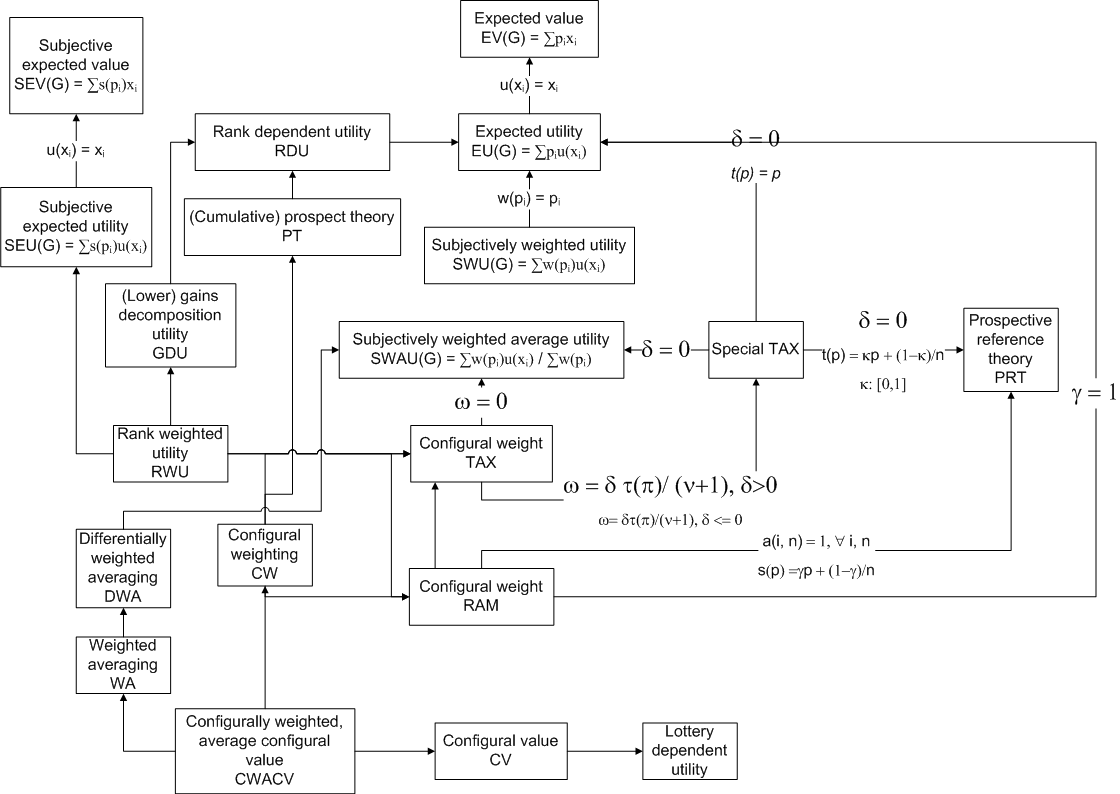
\includegraphics[scale=1.2,width=1.4\textwidth]{correspondence_limits}}
\caption{Correspondence limits for theories of risky decision making.\label{fig:correspondence_limits}}
\end{figure}
\label{correspondence_limits_figure}
\end{landscape}

\subsection{Expected value (EV)}

The basic unit of risky decision making is the gamble.
A gamble $G=(x_1, p_1; x_2, p_2; \ldots, x_n, p_n)$ is a set of $n$ objective consequences $x_i$ with the
probability of each objective consequence being $p_i$ and $\sum\limits_{i=1}^{n} p_i = 1$. The individual outcomes $\{x_i, p_i\}$ are considered to be mutually exclusive and exhaustive. Given two or more gambles to choose from, it is assumed a decision maker will prefer the gamble that has the highest
utility.
The EV of a gamble $G$ is the long-run mean, given by

\begin{equation}
EV(G) = \sum_{i=1}^{n} p_i x_i.
\label{ev_equation}
\end{equation}

Empirical studies provide evidence that decision makers do not maximise expected value when faced with individual choices but the principle becomes increasingly salient when decision makers are faced with a large ($> 10$) \citep*{Montgomery_Adelbratt_1982} number of repeated choices \citep*{Lichtenstein_Slovic_Zink_1969, Li_2003, Colbert_Murray_Nieschwietz_2009}. Nearly all decision making research has focussed on single choice rather than repeated choice situations, the latter being more common in game theoretic research (e.g. repeated Prisoner's dilemmas) (although see \citealp[][]{Post_van_den_Assem_Baltussen_Thaler_2008} for a study of path-dependence on decision making). The theories discussed in this paper have been applied to single choice decision situations. An open research question is how to accommodate these theories under a temporal framework where the effects of past and current decisions on future decisions can be predicted, incorporating the effects of learning \cite[see Problem 6][p. 665]{Hastie_2001}.

\subsection{Expected utility (EU)}


An analysis of the St. Petersburg paradox led \cite{Bernoulli_1738_1954} to develop EU.
An axiomatic formulation of EU assuming completeness, transitivity, continuity and independence was subsequently developed \citep[p. 26]{von_Neumann_Morgenstern_1947}. The EU of a gamble $G$ is given by

\begin{equation}
EU(G) = \sum_{i=1}^{n} p_i u(x_i).
\label{eu_equation}
\end{equation}

If $u(x_i) = x_i$ then the EU reduces to EV.

\subsection{Subjective weighted utility (SWU)}

\cite{Edwards_1954, Edwards_1962} proposed a more general form to allow for probability weightings $w(p_i)$ defined by

\begin{equation}
SWU(G) = \sum_{i=1}^{n} w(p_i) u(x_i),
\label{swu_equation}
\end{equation}

with SWU reducing to EU when $w(p_i) = p_i$.

SWU has a similar form to subjective expected utility \cite{Savage_1954}, given by

\begin{equation}
SEU(G) = \sum_{i=1}^{n} S(p_i) u(x_i).
\label{seu_equation}
\end{equation}

However, the $S(p_i)$ in SEU represents a subjective probability rather a probability weighting $w(p_i)$.
When $u(x_i) = x_i$ SEU reduces to subjective expected value theory \citep*{Preston_Baratta_1948}, given by

\begin{equation}
SEV(G) = \sum_{i=1}^{n} S(p_i) x_i.
\label{sev_equation}
\end{equation}

\subsection{Rank-dependent utility (RDU)}

\cite{Quiggin_1982, Quiggin_1985, Quiggin_1993} used ranks to explain the Allais paradoxes without transparently violating first-order stochastic dominance. First gamble outcomes are arranged from the best outcome to the worst.
A rank is the probability of a gamble yielding an outcome better than a worse outcome. Rather than use probability weightings of individual probabilities, RDU first computes the differences in ranks, and applies a probability weighting to
this difference. For strictly positive gambles $x_1 \geq x_2 \geq \ldots \geq x_n \geq 0$, the RDU of a gamble $G$ is given by

\begin{equation}
\begin{split}
RDU(G) &= \sum_{i=1}^{n} \Bigg[ w^+\Bigg(p_i + \ldots + p_1\Bigg) - w^+\Bigg(p_{i-1} + \ldots + p_1\Bigg)\Bigg] u(x_i)\\
 &= \sum_{i=1}^{n} \Bigg[ w^+\Bigg(\sum_{j=1}^{i} p_j\Bigg) - w^+\Bigg(\sum_{j=1}^{i-1} p_j\Bigg)\Bigg] u(x_i),
\end{split}
\label{rdu_positive_equation}
\end{equation}

where $w^+(p_i)$ is a monotonically increasing function with boundary conditions $w^+(0) = 0$ and $w^+(1) = 1$.
Similarly, for strictly negative gambles $x_1 \leq x_2 \leq \ldots \leq x_n \leq 0$, the RDU is given by

\begin{equation}
\begin{split}
RDU(G) &= \sum_{i=1}^{n} \Bigg[ w^-\Bigg(p_i + \ldots + p_1\Bigg) - w^-\Bigg(p_{i-1} + \ldots + p_1\Bigg)\Bigg] u(x_i)\\
 &= \sum_{i=1}^{n} \Bigg[ w^-\Bigg(\sum_{j=1}^{i} p_j\Bigg) - w^-\Bigg(\sum_{j=1}^{i-1} p_j\Bigg)\Bigg] u(x_i).
\end{split}
\label{rdu_negative_equation}
\end{equation}

RDU reduces to EU when $w^\pm(p_i) = p_i$.

\subsection{Prospect theory utility (PTU)}

\cite{Tversky_Kahneman_1992} incorporated theoretical developments from \cite{Gilboa_1987} and \cite{Schmeidler_1989} to develop PT, providing the ability to model decision making under uncertainty. The outcomes in 
a gamble are ranked such that $x_1 \ge \cdots \ge x_k \ge 0 \ge x_{k+1} \ge \cdots \ge x_n$ and $0 \le k \le n$. The utility of a gamble $G$ is the sum of two RDU terms and is given by

\begin{equation}
\begin{split} 
PTU(G) &= \sum_{i=1}^{n} \Bigg[ w^+ \Bigg(p_i + \ldots + p_1\Bigg) - w^+\Bigg(p_{i-1} + \ldots + p_1\Bigg) \Bigg] u(x_i) \\
 & + \sum_{j=n+1}^{m} \Bigg[ w^- \Bigg(p_i + \ldots + p_{n+1}\Bigg) - w^-\Bigg(p_{i-1} + \ldots + p_{n+1}\Bigg) \Bigg] u(x_i)\\
&= \sum_{i=1}^{n} \Bigg[ w^+ \Bigg(\sum_{j=1}^{i} p_j\Bigg) - w^+\Bigg(\sum_{j=1}^{i-1} p_j\Bigg) \Bigg] u(x_i) \\
 & + \sum_{i=n+1}^{m} \Bigg[ w^- \Bigg(\sum_{j=n+1}^{i} p_j\Bigg) - w^-\Bigg(\sum_{j=n+1}^{i-1} p_j\Bigg) \Bigg] u(x_j).
\end{split}
\label{ptu_equation}
\end{equation}

Under PT loss aversion is modelled by the assumption

\begin{equation}
u(x) =
\begin{cases}
x^\alpha, &\text{if $x \geq 0$}\\
-\lambda (-x)^\beta, &\text{if $x < 0$},
\end{cases}
\label{pt_utility_function} 
\end{equation}

where $\lambda$ is the loss aversion coefficient (see \citet[][p. 1336]{Wakker_2008} for a review of the power utility family).

\subsection{Subjectively weighted average utility (SWAU)}

\citet[][p. 35]{Birnbaum_1999} describes the SWAU model \citep*{Karmarkar_1978, Karmarkar_1979, Viscusi_1989, Lattimore_Baker_Witte_1992}, where the relative weight of an outcome probability in a gamble $G$ depends on the other outcome probabilities in the gamble. The SWAU is given by

\begin{equation}
SWAU(G) = \frac{\displaystyle \sum\limits_{i=1}^{n} w(p_i) u(x_i)}{\displaystyle \sum\limits_{i=1}^{n} w(p_i)}.
\label{swau_equation}
\end{equation}

When $w(p_i) = p_i$, SWAU reduces to EU.

\subsection{Rank-affected multiplicative weights utility (RAMU)}

Given a set of ranked outcomes $x_1 \geq x_2 \geq \ldots \geq x_n$, the RAMU is given by \cite{Birnbaum_2008} as

\begin{equation}
RAMU(G) = \frac{\displaystyle \sum\limits_{i=1}^{n} a(i, n, s_i) t(p_i) u(x_i)}{\displaystyle \sum\limits_{i=1}^{n} a(i, n, s_i) t(p_i)}.
\label{ramu_equation}
\end{equation}

Here the $a(i, n, s_i)$ are the rank and augmented sign branch weights.
The branch probability weighting function $t(p)$ is usually approximated by a power function $t(p) = p^\gamma$. If $\gamma = 1$ and $a(i, n, s_i) = 1$ then RAMU reduces to EU.

\subsection{(Special) transfer of attention exchange utility (TAXU)}

The general TAX formula is given by \cite{Birnbaum_2008} as

\begin{equation}
TAXU(G) = \frac{\displaystyle \sum\limits_{i=1}^{n} t(p_i) u(x_i) + \sum\limits_{i=1}^{n} \sum\limits_{k=1}^{i} \Bigg[ u(x_i) - u(x_k) \Bigg] \omega(p_i, p_k, n) }{\displaystyle \sum\limits_{i=1}^{n} t(p_i)}.
\label{taxu_equation}
\end{equation}

If $\omega = 0$ then this reduces to SWAU.
The special TAX case occurs with the assumption

\begin{equation}
\omega(p_i, p_k, n) =
\begin{cases}
\frac{\displaystyle \delta \cdot t(p_k)}{\displaystyle n+1}, &\text{if $\delta > 0$}\\ \\
\frac{\displaystyle \delta \cdot t(p_i)}{\displaystyle n+1}, &\text{if $\delta \leq 0$}.
\end{cases}
\label{staxu_assumption}
\end{equation}

If $t(p) = p$ and $\delta = 0$ then TAX reduces to EU.
If $\delta = 0$ then TAX reduces to SWAU.
PT, RAM and TAX are special cases of a general configural weighting model discussed in \citet[][p. 91-92]{Birnbaum_2004}, given by

\begin{equation}
CWU(G) = \frac{\displaystyle \sum\limits_{i=1}^{n} w(p_i, G) u(x_i)}{\displaystyle \sum\limits_{i=1}^{n} w(p_i, G)},
\label{general_cwu_equation}
\end{equation}

where the objective consequences are ranked $x_1 > x_2 > \ldots > x_n$ and $w(p_i, G)$ is the branch configural weight of objective consequence $x_i$.
This theory in turn is a specific case of the configurally weighted, average configural value utility model \cite[p. 40]{Birnbaum_1999} given by

\begin{equation}
CWACVU(G) = \frac{\displaystyle \sum\limits_{i=1}^{n} w(x_i, G) u(x_i, G)}{\displaystyle \sum\limits_{i=1}^{n} w(x_i, G)}.
\label{general_cwacvu_equation}
\end{equation}

Configural value models occur when $w(x_i, G) = w(p_i)$ in Eq. \eqref{general_cwacvu_equation} and are given by

\begin{equation}
CVU(G) = \frac{\displaystyle \sum\limits_{i=1}^{n} w(p_i) u(x_i, G)}{\displaystyle \sum\limits_{i=1}^{n} w(p_i)}.
\label{general_cvu_equation}
\end{equation}

The lottery-dependent utility of \cite{Becker_Sarin_1987} occurs when $w(p_i) = p_i$ in Eq. \eqref{general_cvu_equation} and is given by

\begin{equation}
LDU(G) = \frac{\displaystyle \sum\limits_{i=1}^{n} p_i u(x_i, G)}{\displaystyle \sum\limits_{i=1}^{n} p_i}.
\label{ldu_equation}
\end{equation}

Weighted averaging models occur when $u(x_i, G) = u(x_i)$ in Eq. \eqref{general_cwacvu_equation} and are given by

\begin{equation}
WAU(G) = \frac{\displaystyle \sum\limits_{i=1}^{n} w(x_i, G) u(x_i)}{\displaystyle \sum\limits_{i=1}^{n} w(x_i, G)}.
\label{general_wau_equation}
\end{equation}

Differentially weighted averaging models occur when $w(x_i, G) = w(x_i, p_i)$ and $u(x_i, G) = u(x_i)$ in Eq. \eqref{general_wau_equation}:

\begin{equation}
DWAU(G) = \frac{\displaystyle \sum\limits_{i=1}^{n} w(x_i, G) u(x_i)}{\displaystyle \sum\limits_{i=1}^{n} w(x_i, G)}.
\label{general_dwau_equation}
\end{equation}

The constant weighting or SWAU model of Eq. \eqref{swau_equation} occurs when $w(x_i, G) = w(x_i, p_i) = w(p_i)$ in \eqref{general_dwau_equation}.

\subsection{Prospective reference theory utility (PRTU)}

The \cite{Viscusi_1989} PRT is the sum of a weighted EU term and a weighted average of the outcome utilities and is given by

\begin{equation}
PRTU(G) = \gamma \sum\limits_{i=1}^{n} p_i u(x_i) + (1-\gamma) \sum\limits_{i=1}^{n} \displaystyle\frac{u(x_i)}{n}.
\label{prtu_equation}
\end{equation}

PRT is a special case of RAM, when $a(i, n) = 1 \forall i, n$ and $\delta(p) = \gamma p + \frac{(1-\gamma)}{n}$.
PRT is also a special case of TAX, when $\delta = 0$ and $t(p) = \gamma p + \frac{(1-\gamma)}{n}$.
When $\gamma = 1$, PRT reduces to EU. In PRT, the probability weightings are unaffected by rank.

\subsection{(Lower) gains decomposition utility (GDU)}

\citet[][p. 202]{Luce_2000} devised a process to iteratively decompose a multi-branch gamble into a series of binary gambles (see also \cite{Marley_Luce_2001, Marley_Luce_2005, Luce_Marley_2005}), and provided an induction formula to compute the utility of a gamble $G=(x_1,p_1; x_2, p_2; \ldots; x_n, p_n)$ with $n$ outcomes as

\begin{equation}
GDU(G) = \sum_{j=0}^{n-1} GDU(x_1,p_1; \ldots;x_{n-j},p_{n-j}) \Bigg[1 - w\Bigg(\frac{\displaystyle \sum_{i=1}^{n-j-1} p_i}{\displaystyle \sum_{i=1}^{n-j} p_i} \Bigg)\Bigg] \prod_{i=0}^{j-1} w\Bigg(\frac{\displaystyle \sum_{k=1}^{n-i-1} p_k}{\displaystyle \sum_{k=1}^{n-i} p_k} \Bigg).
\label{gdu_equation}
\end{equation}

For binary gambles, this induction formula reduces to 

\begin{equation}
GDU(G) = w(p_1) u(x_1) + w(1-p_1) u(x_2),
\label{gdu_binary_equation}
\end{equation}

which is equivalent to binary RDU \cite[p. 143]{Marley_Luce_2001}.
RDU is a special case of GDU where the GDU weights take on a specific form.

As the {\bf pt} package has an object-oriented design, it would be straightfoward to incorporate other risky decision making theories for comparison.

\section{The R package pt}

This package contains six classes: {\tt Utility}, {\tt ProbWeight}, {\tt Outcome}, {\tt Gamble}, {\tt Gambles} and {\tt Choices}. Only {\tt Utility}, {\tt ProbWeight} and {\tt Choices} are directly modifiable.
These classes have been designed to capture risky decision making structure. {\tt Outcome}, {\tt Gamble}, {\tt Gambles} and {\tt Choices} are arranged hierarchically. At the highest level sits the {\tt Choices} class, which is a container for the {\tt Gambles} class. A {\tt Choices} object can
be used to compare the results of different decision making scenarios. For instance one can use a {\tt Choices} object to explore the Allais paradoxes. The paradoxes involve two separate situations, with each situation involving a decision between gambles. The {\tt Gambles} class is a container for {\tt Gamble} class objects. The {\tt Gambles} class can be used as an input for calculating the utilities and certainty equivalents of gambles under different decision making theories. Each {\tt Gamble} class object in turn contains a vector of {\tt Outcome} class objects. Each {\tt Outcome} class object stores information such as probabilities, objective outcomes and calculational variables for risky decision making theories.

The {\tt Utility} and {\tt ProbWeight} classes generate utility and probability weighting objects with different functional forms and parameterisations. These objects can be used to explore the parameter spaces of different risky decision making theories.

{\tt Choices} class objects can be created dynamically or read from external text files. They can also be saved to external
text files for refererence.

The package has extensive visualisation capabilities. {\tt Choices} class objects can be visualised as decision nodes leading to one-stage decision trees.

Individual probability weighting functions and families of probability weighting functions can be plotted. Individual utility functions can also be plotted. Certainty equivalents and risk premiums can be plotted. Finally the
probability simplex can be plotted along with indifference curves.

The decision making theories currently implemented are EV, EU, SWU, RDU, PT, SWAU, RAM, TAX, PRT and GDU.

Some key features of the package include the capability to input a practically unlimited number of choices, and also the
capability to compute ranks of gamble outcomes. The computation of ranks has historically made it difficult
for many people to work with PT, however these issues have been addressed in the {\bf pt} package. At its most basic level,
the {\bf pt} package can be used to compute nothing more than the PT utilities for general gambles, alleviating a major problem for
students of PT. Students can concentrate on the psychological concepts introduced by Kahneman and Tversky rather than being caught up in performing intricate mathematical calculations.

Finally the \cite{Birnbaum_1997} recipe for generating gambles violating stochastic dominance has been implemented.

\section{Validation tests}

Published literature was used to validate the {\bf pt} package. The calculations in \cite{Birnbaum_1999}, \cite{Birnbaum_Patton_Lott_1999}, \cite{Wakker_2003}, \cite{Birnbaum_2005a}, \cite{Birnbaum_2007}, \cite{Birnbaum_Bahra_2007}, \cite{Birnbaum_2008}, \cite{Birnbaum_Schmidt_2008}, \cite{Birnbaum_2010} and \cite{Wakker_2010} were used to validate the methods. These examples have been included as tests in the {\bf pt} package. Calculations were also cross checked for consistency against the basic RAM, TAX and PT calculators available at
Birnbaum's website (\url{http://psych.fullerton.edu/mbirnbaum/calculators/}), 
K\"{o}bberling's basic PT calculator at Wakker's website \url{http://people.few.eur.nl/wakker/miscella/calculate.cpt.kobb/index.htm} and Sewell's basic PT calculators available at \url{http://prospect-theory.behaviouralfinance.net/}.

\section{The Allais paradoxes}

To illustrate the usage of the {\bf pt} package the Allais paradoxes will be presented. 
Prospect theory gained widespread attention as it was the first theory to explain the Allais paradoxes. EU cannot explain these paradoxes. These paradoxes are examples of critical tests \citep*{Birnbaum_2011} as no functional forms or parameterisations need to be estimated to show internal inconsistencies in EU.

\subsection{Common consequence paradox}

First load the {\bf pt} library. In the remainder of the paper all R code is highlighted with a background.

\begin{knitrout}
\definecolor{shadecolor}{rgb}{0.969, 0.969, 0.969}\color{fgcolor}\begin{kframe}
\begin{alltt}
\hlkwd{library}\hlstd{(}\hlstr{"pt"}\hlstd{)}
\end{alltt}
\end{kframe}
\end{knitrout}


Consider problems 1 and 2 from \citet[][p. 265-266]{Kahneman_Tversky_1979}, representing the common consequence paradox. This can be modelled using {\bf pt} as follows.

\begin{knitrout}
\definecolor{shadecolor}{rgb}{0.969, 0.969, 0.969}\color{fgcolor}\begin{kframe}
\begin{alltt}
\hlstd{choice_ids} \hlkwb{<-} \hlkwd{c}\hlstd{(}\hlnum{1}\hlstd{,} \hlnum{1}\hlstd{,} \hlnum{1}\hlstd{,} \hlnum{1}\hlstd{,} \hlnum{2}\hlstd{,} \hlnum{2}\hlstd{,} \hlnum{2}\hlstd{,} \hlnum{2}\hlstd{)}
\hlstd{gamble_ids} \hlkwb{<-} \hlkwd{c}\hlstd{(}\hlnum{1}\hlstd{,} \hlnum{1}\hlstd{,} \hlnum{1}\hlstd{,} \hlnum{2}\hlstd{,} \hlnum{1}\hlstd{,} \hlnum{1}\hlstd{,} \hlnum{2}\hlstd{,} \hlnum{2}\hlstd{)}
\hlstd{outcome_ids} \hlkwb{<-} \hlkwd{c}\hlstd{(}\hlnum{1}\hlstd{,} \hlnum{2}\hlstd{,} \hlnum{3}\hlstd{,} \hlnum{1}\hlstd{,} \hlnum{1}\hlstd{,} \hlnum{2}\hlstd{,} \hlnum{1}\hlstd{,} \hlnum{2}\hlstd{)}
\hlstd{objective_consequences} \hlkwb{<-} \hlkwd{c}\hlstd{(}\hlnum{2500}\hlstd{,} \hlnum{2400}\hlstd{,} \hlnum{0}\hlstd{,} \hlnum{2400}\hlstd{,}
        \hlnum{2500}\hlstd{,} \hlnum{0}\hlstd{,} \hlnum{2400}\hlstd{,} \hlnum{0}\hlstd{)}
\hlstd{probability_strings} \hlkwb{<-} \hlkwd{c}\hlstd{(}\hlstr{"0.33"}\hlstd{,} \hlstr{"0.66"}\hlstd{,} \hlstr{"0.01"}\hlstd{,} \hlstr{"1.0"}\hlstd{,}
        \hlstr{"0.33"}\hlstd{,} \hlstr{"0.67"}\hlstd{,} \hlstr{"0.34"}\hlstd{,} \hlstr{"0.66"}\hlstd{)}
\hlstd{my_choices} \hlkwb{<-} \hlkwd{Choices}\hlstd{(}\hlkwc{choice_ids}\hlstd{=choice_ids,}
        \hlkwc{gamble_ids}\hlstd{=gamble_ids,}
        \hlkwc{outcome_ids}\hlstd{=outcome_ids,}
        \hlkwc{objective_consequences}\hlstd{=objective_consequences,}
        \hlkwc{probability_strings}\hlstd{=probability_strings)}
\hlstd{my_choices}
\end{alltt}
\begin{verbatim}
##   cid gid oid   pr   oc
## 1   1   1   1 0.33 2500
## 2   1   1   2 0.66 2400
## 3   1   1   3 0.01    0
## 4   1   2   1  1.0 2400
## 5   2   1   1 0.33 2500
## 6   2   1   2 0.67    0
## 7   2   2   1 0.34 2400
## 8   2   2   2 0.66    0
\end{verbatim}
\begin{alltt}
\hlkwd{drawChoices}\hlstd{(my_choices,}
        \hlkwc{decision_square_x}\hlstd{=}\hlnum{0.2}\hlstd{,} \hlkwc{decision_square_edge_length}\hlstd{=}\hlnum{0.05}\hlstd{,}
        \hlkwc{circle_radius}\hlstd{=}\hlnum{0.025}\hlstd{,} \hlkwc{y_split_gap}\hlstd{=}\hlnum{0.1}\hlstd{,} \hlkwc{x_split_offset}\hlstd{=}\hlnum{0.03}\hlstd{,}
        \hlkwc{probability_text_digits}\hlstd{=}\hlnum{4}\hlstd{,} \hlkwc{y_probability_text_offset}\hlstd{=}\hlnum{0.015}\hlstd{,}
        \hlkwc{y_value_text_offset}\hlstd{=}\hlnum{0.005}\hlstd{,} \hlkwc{x_value_text_offset}\hlstd{=}\hlnum{0.025}\hlstd{,}
        \hlkwc{probability_text_font_colour}\hlstd{=}\hlstr{"red"}\hlstd{,} \hlkwc{probability_text_font_size}\hlstd{=}\hlnum{11}\hlstd{,}
        \hlkwc{objective_consequence_text_font_colour}\hlstd{=}\hlstr{"blue"}\hlstd{,}
        \hlkwc{objective_consequence_text_font_size}\hlstd{=}\hlnum{11}\hlstd{,} \hlkwc{label}\hlstd{=}\hlkwd{c}\hlstd{(}\hlstr{"A"}\hlstd{,}\hlstr{"B"}\hlstd{,}\hlstr{"C"}\hlstd{,} \hlstr{"D"}\hlstd{),}
        \hlkwc{label_font_colour}\hlstd{=}\hlkwd{c}\hlstd{(}\hlstr{"orange"}\hlstd{,}\hlstr{"magenta"}\hlstd{,}\hlstr{"green"}\hlstd{,}\hlstr{"blue"}\hlstd{),}
        \hlkwc{label_font_size}\hlstd{=}\hlkwd{c}\hlstd{(}\hlnum{11}\hlstd{,}\hlnum{11}\hlstd{,}\hlnum{11}\hlstd{,}\hlnum{11}\hlstd{),}
        \hlkwc{label_positions}\hlstd{=}\hlkwd{list}\hlstd{(}\hlkwd{c}\hlstd{(}\hlnum{0.26}\hlstd{,}\hlnum{0.85}\hlstd{),}\hlkwd{c}\hlstd{(}\hlnum{0.26}\hlstd{,}\hlnum{0.55}\hlstd{),}
                \hlkwd{c}\hlstd{(}\hlnum{0.26}\hlstd{,}\hlnum{0.4}\hlstd{),}\hlkwd{c}\hlstd{(}\hlnum{0.26}\hlstd{,}\hlnum{0.1}\hlstd{)))}
\end{alltt}
\end{kframe}

{\centering 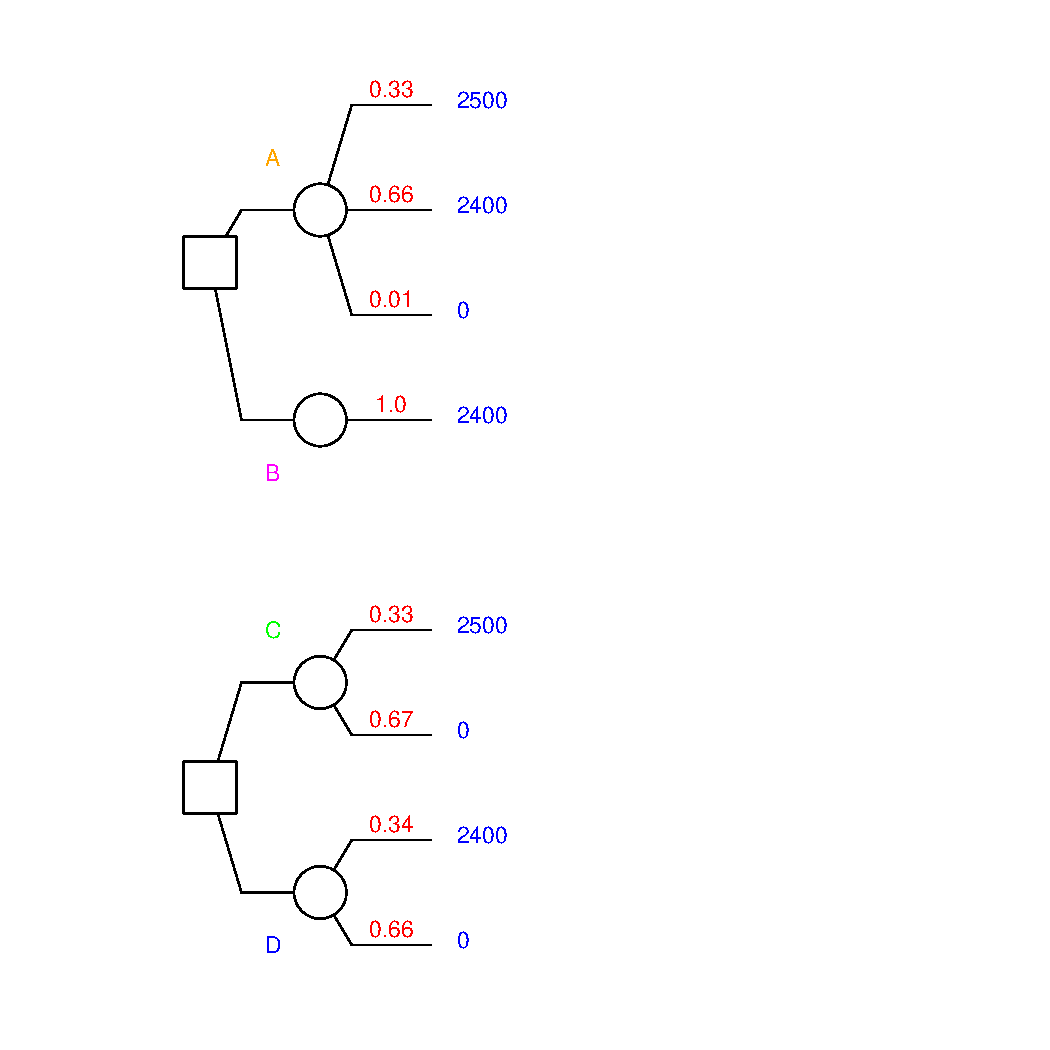
\includegraphics[width=0.8\linewidth]{figure/unnamed-chunk-2} 

}



\end{knitrout}


In a group of $72$ subjects, $82\%$ preferred $B > A$ and $83\%$ preferred $C > D$, with $61\%$ of the individuals
making the majority (modal) choices across both conditions. Compare the EV for each gamble in the two choices.

\begin{knitrout}
\definecolor{shadecolor}{rgb}{0.969, 0.969, 0.969}\color{fgcolor}\begin{kframe}
\begin{alltt}
\hlkwd{compareEV}\hlstd{(my_choices,} \hlkwc{digits}\hlstd{=}\hlnum{4}\hlstd{)}
\end{alltt}
\begin{verbatim}
##   cid gid   ev
## 1   1   1 2409
## 2   1   2 2400
## 3   2   1  825
## 4   2   2  816
\end{verbatim}
\end{kframe}
\end{knitrout}


Here {\tt cid} represents the choice id ({\tt cid} 1 represents the upper decision tree and {\tt cid} 2 represents the lower decision tree), {\tt gid} is the gamble id (in the upper decision tree {\tt gid} 1 represents gamble A and {\tt gid} 2 represents gamble B, while in the lower decision tree {\tt gid} 1 represents gamble C and {\tt gid} 2 represents gamble D), and {\tt ev} is the expected value of each gamble. Gambles $A$ and $C$ have the highest EV, but empirically people are preferring the certainty of $B$ to the uncertainty of $A$ (the certainty effect). Compute the EU using a hypothetical concave utility function.

\begin{knitrout}
\definecolor{shadecolor}{rgb}{0.969, 0.969, 0.969}\color{fgcolor}\begin{kframe}
\begin{alltt}
\hlstd{my_utility} \hlkwb{<-} \hlkwd{Utility}\hlstd{(}\hlkwc{fun}\hlstd{=}\hlstr{"power"}\hlstd{,} \hlkwc{par}\hlstd{=}\hlkwd{c}\hlstd{(}\hlkwc{alpha}\hlstd{=}\hlnum{0.63}\hlstd{,} \hlkwc{beta}\hlstd{=}\hlnum{0.63}\hlstd{,} \hlkwc{lambda}\hlstd{=}\hlnum{2.25}\hlstd{))}
\hlkwd{compareEU}\hlstd{(my_choices,} \hlkwc{utility}\hlstd{=my_utility,} \hlkwc{digits}\hlstd{=}\hlnum{4}\hlstd{)}
\end{alltt}
\begin{verbatim}
##   cid gid   ev    eu    ce                 rp
## 1   1   1 2409 134.6  2395              14.34
## 2   1   2 2400 134.8  2400 0.0000000000009095
## 3   2   1  825 45.63 430.2              394.8
## 4   2   2  816 45.82   433                383
\end{verbatim}
\end{kframe}
\end{knitrout}


EU predicts the preferences $B > A$ and $D > C$.
Here {\tt eu} is the expected utility of the gamble, {\tt ce} is the certainty equivalent (quantifying the degree of risk aversion or seeking exhibited by a decision maker) and
{\tt rp} is the risk premium (the difference between the expected value and certainty equivalent). Intuitively, \citet[][p. 248]{Yates_1990} defines the risk premium as ``the amount of expected value the decision maker is willing to ``give up'', perhaps to avoid the risk entailed by the prospect [gamble]". Risk
averse decision makers have a positive risk premium, risk neutral decision makers have a
risk premium of zero (they are indifferent to risk) and risk seeking decision makers have a negative risk
premium. In EU risk aversion is modelled using concave utility functions, representing diminishing marginal utility. However, in other theories such as RDU, risk aversion can arise using convex utility functions and probability weightings (e.g. see \citet[][p. 52-53, 71-3, 175-176]{Wakker_2010}). With a hypothetical
convex utility function, EU predicts the preferences $A > B$ and $C > D$.

\begin{knitrout}
\definecolor{shadecolor}{rgb}{0.969, 0.969, 0.969}\color{fgcolor}\begin{kframe}
\begin{alltt}
\hlstd{my_utility} \hlkwb{<-} \hlkwd{Utility}\hlstd{(}\hlkwc{fun}\hlstd{=}\hlstr{"power"}\hlstd{,} \hlkwc{par}\hlstd{=}\hlkwd{c}\hlstd{(}\hlkwc{alpha}\hlstd{=}\hlnum{1.2}\hlstd{,} \hlkwc{beta}\hlstd{=}\hlnum{1.2}\hlstd{,} \hlkwc{lambda}\hlstd{=}\hlnum{2.25}\hlstd{))}
\hlkwd{compareEU}\hlstd{(my_choices,} \hlkwc{utility}\hlstd{=my_utility,} \hlkwc{digits}\hlstd{=}\hlnum{4}\hlstd{)}
\end{alltt}
\begin{verbatim}
##   cid gid   ev    eu    ce     rp
## 1   1   1 2409 11458  2413 -4.129
## 2   1   2 2400 11383  2400      0
## 3   2   1  825  3945 992.4 -167.4
## 4   2   2  816  3870 976.7 -160.7
\end{verbatim}
\end{kframe}
\end{knitrout}


With a hypothetical linear utility function $u(x)=x$, EU reduces to EV.

\begin{knitrout}
\definecolor{shadecolor}{rgb}{0.969, 0.969, 0.969}\color{fgcolor}\begin{kframe}
\begin{alltt}
\hlstd{my_utility} \hlkwb{<-} \hlkwd{Utility}\hlstd{(}\hlkwc{fun}\hlstd{=}\hlstr{"power"}\hlstd{,} \hlkwc{par}\hlstd{=}\hlkwd{c}\hlstd{(}\hlkwc{alpha}\hlstd{=}\hlnum{1.0}\hlstd{,} \hlkwc{beta}\hlstd{=}\hlnum{1.0}\hlstd{,} \hlkwc{lambda}\hlstd{=}\hlnum{1.0}\hlstd{))}
\hlkwd{compareEU}\hlstd{(my_choices,} \hlkwc{utility}\hlstd{=my_utility,} \hlkwc{digits}\hlstd{=}\hlnum{4}\hlstd{)}
\end{alltt}
\begin{verbatim}
##   cid gid   ev   eu   ce rp
## 1   1   1 2409 2409 2409  0
## 2   1   2 2400 2400 2400  0
## 3   2   1  825  825  825  0
## 4   2   2  816  816  816  0
\end{verbatim}
\end{kframe}
\end{knitrout}


In choice 1 if decision makers are preferring $B > A$, this implies (applying the expected utility formula of Eq. \eqref{eu_equation}) that

\begin{equation}
\begin{split}
EU(B) &> EU(A)\\
1.0 \times u(2400) &> 0.33 \times u(2500) + 0.66 \times u(2400) + 0.01 \times u(0)\\
0.34 \times u(2400) &> 0.33 \times u(2500) + 0.01 \times u(0),
\end{split}
\end{equation}

subtracting $0.66 \times u(2400)$ from both sides of the inequality.
In choice 2 if decision makers are preferring $C > D$, this implies that

\begin{equation}
\begin{split}
EU(C) &> EU(D)\\
0.33 \times u(2500) + 0.67 \times u(0) &> 0.34 \times u(2400) + 0.66 \times u(0)\\
0.33 \times u(2500) + 0.01 \times u(0) &> 0.34 \times u(2400),
\end{split}
\end{equation}

subtracting $0.66 \times u(0)$ from both sides of the inequality.
The inequalities are reversed across the two choice situations, no matter what functional form and parameterisation is used for the expected utility function $u$. Expected utility predicts that people will either choose $A > B$ and $C > D$ or choose $B > A$ and $D > C$ if the independence axiom holds. It does not predict the empirically observed pattern of choices. This pattern has been replicated in a number of studies \cite[e.g. see][]{MacCrimmon_Larsson_1979}. In contrast compute the PTU.

\begin{knitrout}
\definecolor{shadecolor}{rgb}{0.969, 0.969, 0.969}\color{fgcolor}\begin{kframe}
\begin{alltt}
\hlstd{tk_1992_utility} \hlkwb{<-} \hlkwd{Utility}\hlstd{(}\hlkwc{fun}\hlstd{=}\hlstr{"power"}\hlstd{,} \hlkwc{par}\hlstd{=}\hlkwd{c}\hlstd{(}\hlkwc{alpha}\hlstd{=}\hlnum{0.88}\hlstd{,} \hlkwc{beta}\hlstd{=}\hlnum{0.88}\hlstd{,} \hlkwc{lambda}\hlstd{=}\hlnum{2.25}\hlstd{))}
\hlstd{linear_in_log_odds_prob_weight} \hlkwb{<-} \hlkwd{ProbWeight}\hlstd{(}\hlkwc{fun}\hlstd{=}\hlstr{"linear_in_log_odds"}\hlstd{,} \hlkwc{par}\hlstd{=}\hlkwd{c}\hlstd{(}\hlkwc{alpha}\hlstd{=}\hlnum{0.61}\hlstd{,} \hlkwc{beta}\hlstd{=}\hlnum{0.724}\hlstd{))}
\hlkwd{comparePT}\hlstd{(my_choices,}
        \hlkwc{prob_weight_for_positive_outcomes}\hlstd{=linear_in_log_odds_prob_weight,}
        \hlkwc{prob_weight_for_negative_outcomes}\hlstd{=linear_in_log_odds_prob_weight,}
        \hlkwc{utility}\hlstd{=tk_1992_utility,} \hlkwc{digits}\hlstd{=}\hlnum{4}\hlstd{)}
\end{alltt}
\begin{verbatim}
##   cid gid   ev    pt    ce                 rp
## 1   1   1 2409 881.3  2222                187
## 2   1   2 2400 943.2  2400 -0.000000000001819
## 3   2   1  825 312.6 684.2              140.8
## 4   2   2  816 307.2 670.9              145.1
\end{verbatim}
\end{kframe}
\end{knitrout}


PT predicts the preferences $B > A$ and $C > D$, in line with the empirical data.
Given there are three objective consequences in this example $\{0, 2400, 2500\}$, they can be displayed in the probability simplex \citep*{Marschak_1950, Machina_1987} as follows.

\begin{knitrout}
\definecolor{shadecolor}{rgb}{0.969, 0.969, 0.969}\color{fgcolor}\begin{kframe}
\begin{alltt}
\hlstd{my_utility} \hlkwb{<-} \hlkwd{Utility}\hlstd{(}\hlkwc{fun}\hlstd{=}\hlstr{"power"}\hlstd{,} \hlkwc{par}\hlstd{=}\hlkwd{c}\hlstd{(}\hlkwc{alpha}\hlstd{=}\hlnum{0.88}\hlstd{,} \hlkwc{beta}\hlstd{=}\hlnum{0.88}\hlstd{,} \hlkwc{lambda}\hlstd{=}\hlnum{2.25}\hlstd{))}

\hlkwd{drawSimplex}\hlstd{(}\hlkwc{x1}\hlstd{=}\hlnum{0}\hlstd{,} \hlkwc{x2}\hlstd{=}\hlnum{2400}\hlstd{,} \hlkwc{x3}\hlstd{=}\hlnum{2500}\hlstd{,}
        \hlkwc{line_dot_density}\hlstd{=}\hlnum{3000}\hlstd{,}
        \hlkwc{draw_ev_flag}\hlstd{=}\hlnum{TRUE}\hlstd{,} \hlkwc{ev_colour}\hlstd{=}\hlstr{"black"}\hlstd{,}
        \hlkwc{draw_pt_flag}\hlstd{=}\hlnum{TRUE}\hlstd{,} \hlkwc{alpha}\hlstd{=}\hlnum{0.61}\hlstd{,} \hlkwc{beta}\hlstd{=}\hlnum{0.724}\hlstd{,} \hlkwc{pt_colour}\hlstd{=}\hlstr{"red"}\hlstd{,}
        \hlkwc{draw_utility_flag}\hlstd{=}\hlnum{TRUE}\hlstd{,} \hlkwc{utility}\hlstd{=my_utility,} \hlkwc{eu_colour}\hlstd{=}\hlstr{"purple"}\hlstd{,}
        \hlkwc{start_points}\hlstd{=}\hlkwd{list}\hlstd{(}\hlkwd{c}\hlstd{(}\hlnum{0.1}\hlstd{,}\hlnum{0.9}\hlstd{),}\hlkwd{c}\hlstd{(}\hlnum{0.2}\hlstd{,}\hlnum{0.8}\hlstd{),}\hlkwd{c}\hlstd{(}\hlnum{0.3}\hlstd{,}\hlnum{0.7}\hlstd{),}\hlkwd{c}\hlstd{(}\hlnum{0.4}\hlstd{,}\hlnum{0.6}\hlstd{),}
                \hlkwd{c}\hlstd{(}\hlnum{0.5}\hlstd{,}\hlnum{0.5}\hlstd{),}\hlkwd{c}\hlstd{(}\hlnum{0.6}\hlstd{,}\hlnum{0.4}\hlstd{),}\hlkwd{c}\hlstd{(}\hlnum{0.7}\hlstd{,}\hlnum{0.3}\hlstd{),}\hlkwd{c}\hlstd{(}\hlnum{0.8}\hlstd{,}\hlnum{0.2}\hlstd{),}\hlkwd{c}\hlstd{(}\hlnum{0.9}\hlstd{,}\hlnum{0.1}\hlstd{)),}
        \hlkwc{labels}\hlstd{=}\hlkwd{c}\hlstd{(}\hlstr{"A"}\hlstd{,}\hlstr{"B"}\hlstd{,}\hlstr{"C"}\hlstd{,}\hlstr{"D"}\hlstd{,}\hlstr{"increasing preference"}\hlstd{),}
        \hlkwc{label_positions}\hlstd{=}\hlkwd{list}\hlstd{(}\hlkwd{c}\hlstd{(}\hlnum{0.05}\hlstd{,}\hlnum{0.38}\hlstd{),}\hlkwd{c}\hlstd{(}\hlnum{0.05}\hlstd{,}\hlnum{0.05}\hlstd{),}\hlkwd{c}\hlstd{(}\hlnum{0.7}\hlstd{,}\hlnum{0.38}\hlstd{),}
                \hlkwd{c}\hlstd{(}\hlnum{0.7}\hlstd{,}\hlnum{0.05}\hlstd{),}\hlkwd{c}\hlstd{(}\hlnum{0.7}\hlstd{,}\hlnum{0.7}\hlstd{)),}
        \hlkwc{label_colours}\hlstd{=}\hlkwd{c}\hlstd{(}\hlstr{"orange"}\hlstd{,}\hlstr{"magenta"}\hlstd{,}\hlstr{"green"}\hlstd{,}\hlstr{"blue"}\hlstd{,}\hlstr{"red"}\hlstd{),}
        \hlkwc{label_font_sizes}\hlstd{=}\hlkwd{c}\hlstd{(}\hlnum{12}\hlstd{,}\hlnum{12}\hlstd{,}\hlnum{12}\hlstd{,}\hlnum{12}\hlstd{,}\hlnum{16}\hlstd{),}
        \hlkwc{label_font_faces}\hlstd{=}\hlkwd{c}\hlstd{(}\hlstr{"plain"}\hlstd{,}\hlstr{"plain"}\hlstd{,}\hlstr{"plain"}\hlstd{,}\hlstr{"plain"}\hlstd{,}\hlstr{"bold"}\hlstd{),}
        \hlkwc{label_rotations}\hlstd{=}\hlkwd{c}\hlstd{(}\hlnum{0}\hlstd{,}\hlnum{0}\hlstd{,}\hlnum{0}\hlstd{,}\hlnum{0}\hlstd{,}\hlopt{-}\hlnum{45}\hlstd{),}
        \hlkwc{circle_radii}\hlstd{=}\hlkwd{c}\hlstd{(}\hlnum{0.01}\hlstd{,}\hlnum{0.01}\hlstd{,}\hlnum{0.01}\hlstd{,}\hlnum{0.01}\hlstd{),}
        \hlkwc{circle_outline_colours}\hlstd{=}\hlkwd{c}\hlstd{(}\hlstr{"black"}\hlstd{,}\hlstr{"black"}\hlstd{,}\hlstr{"black"}\hlstd{,}\hlstr{"black"}\hlstd{),}
        \hlkwc{circle_fill_colours}\hlstd{=}\hlkwd{c}\hlstd{(}\hlstr{"orange"}\hlstd{,}\hlstr{"purple"}\hlstd{,}\hlstr{"orange"}\hlstd{,}\hlstr{"purple"}\hlstd{),}
        \hlkwc{circle_positions}\hlstd{=}\hlkwd{list}\hlstd{(}\hlkwd{c}\hlstd{(}\hlnum{0.01}\hlstd{,}\hlnum{0.33}\hlstd{),}\hlkwd{c}\hlstd{(}\hlnum{0}\hlstd{,}\hlnum{0}\hlstd{),}
                \hlkwd{c}\hlstd{(}\hlnum{0.67}\hlstd{,}\hlnum{0.33}\hlstd{),}\hlkwd{c}\hlstd{(}\hlnum{0.66}\hlstd{,}\hlnum{0}\hlstd{)),}
        \hlkwc{lines}\hlstd{=}\hlkwd{list}\hlstd{(}\hlkwd{c}\hlstd{(}\hlnum{0.01}\hlstd{,}\hlnum{0.33}\hlstd{,}\hlnum{0}\hlstd{,}\hlnum{0}\hlstd{),}\hlkwd{c}\hlstd{(}\hlnum{0}\hlstd{,}\hlnum{0}\hlstd{,}\hlnum{0.66}\hlstd{,}\hlnum{0}\hlstd{),}
                \hlkwd{c}\hlstd{(}\hlnum{0.66}\hlstd{,}\hlnum{0}\hlstd{,}\hlnum{0.67}\hlstd{,}\hlnum{0.33}\hlstd{),}\hlkwd{c}\hlstd{(}\hlnum{0.67}\hlstd{,}\hlnum{0.33}\hlstd{,}\hlnum{0.01}\hlstd{,}\hlnum{0.33}\hlstd{)),}
        \hlkwc{line_widths}\hlstd{=}\hlkwd{c}\hlstd{(}\hlnum{1}\hlstd{,} \hlnum{1}\hlstd{,} \hlnum{1}\hlstd{,} \hlnum{1}\hlstd{),}
        \hlkwc{line_styles}\hlstd{=}\hlkwd{c}\hlstd{(}\hlstr{"dashed"}\hlstd{,} \hlstr{"dashed"}\hlstd{,} \hlstr{"dashed"}\hlstd{,} \hlstr{"dashed"}\hlstd{),}
        \hlkwc{line_colours}\hlstd{=}\hlkwd{c}\hlstd{(}\hlstr{"blue"}\hlstd{,}\hlstr{"blue"}\hlstd{,}\hlstr{"blue"}\hlstd{,}\hlstr{"blue"}\hlstd{),}
        \hlkwc{arrows}\hlstd{=}\hlkwd{list}\hlstd{(}\hlkwd{c}\hlstd{(}\hlnum{0.8}\hlstd{,}\hlnum{0.5}\hlstd{,}\hlnum{0.5}\hlstd{,}\hlnum{0.8}\hlstd{)),}
        \hlkwc{arrow_widths}\hlstd{=}\hlkwd{c}\hlstd{(}\hlnum{2}\hlstd{),} \hlkwc{arrow_styles}\hlstd{=}\hlkwd{c}\hlstd{(}\hlstr{"solid"}\hlstd{),} \hlkwc{arrow_colours}\hlstd{=}\hlkwd{c}\hlstd{(}\hlstr{"red"}\hlstd{))}
\end{alltt}
\end{kframe}

{\centering 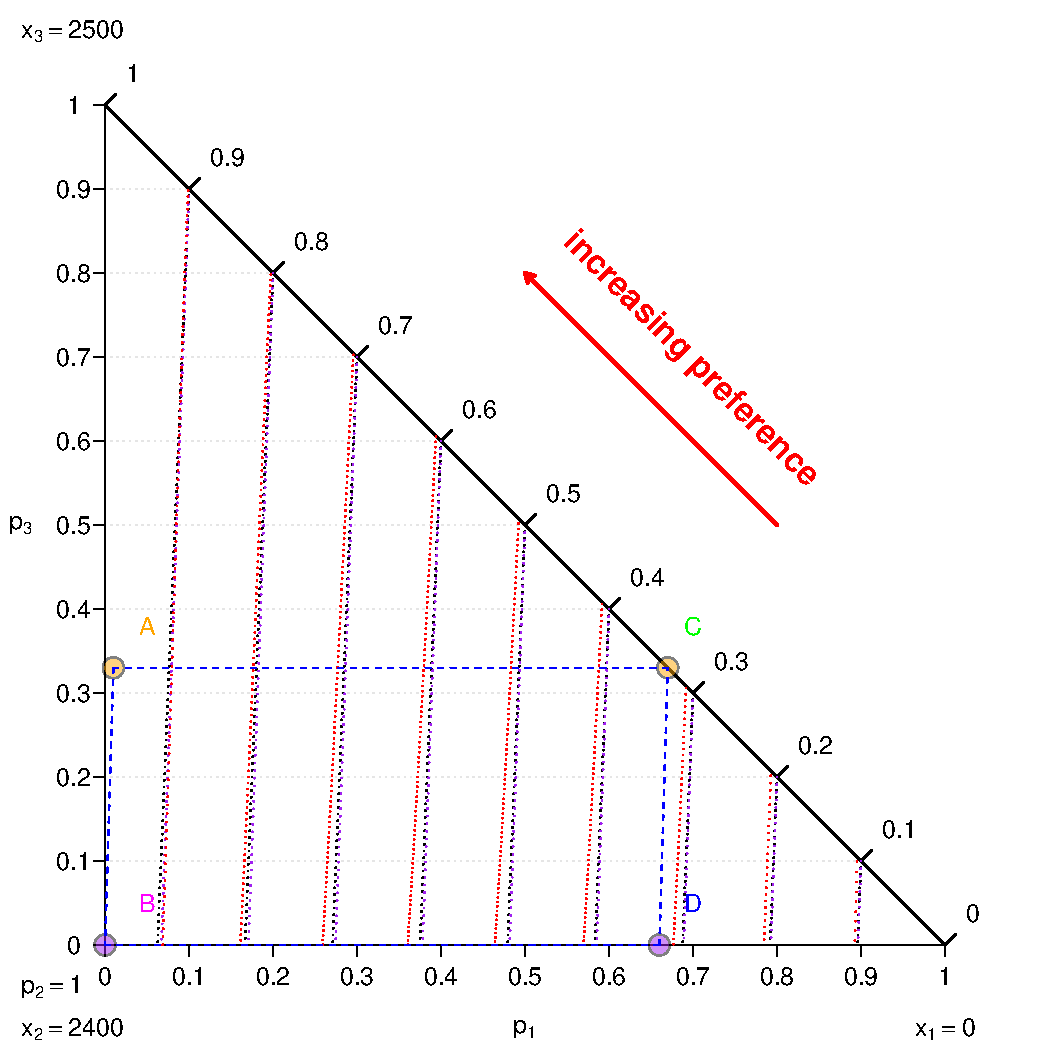
\includegraphics[width=0.8\linewidth]{figure/unnamed-chunk-8} 

}



\end{knitrout}


The iso-expected value lines are shown in black, the expected utility indifference curves (lines) in purple and the prospect theory indifference curves in red. The probability of $x_2$ is $1.0$ at the bottom left hand corner. North-east movement along each iso-expected value line increases the probabilities of $x_3$ and $x_1$ relative to $x_2$. North-west movement increases the probability of the higher outcome $x_3$. The Allais paradoxes arise due to the assumption of linear probabilities in the EU formula Eq. \eqref{eu_equation}. Linear probabilities generate
 indifference curves that are parallel lines in the triangle. Line slopes capture the degree of risk aversion/seeking. Risk neutrality for decision makers is represented by the iso-expected value lines. Risk averse expected utility decision makers have indifference lines that are steeper than the iso-expected value lines. Expected utility risk seekers
have indifference lines that are flatter than the iso-expected value lines. In the first choice, decision
makers exhibit risk aversion, opting for the sure gain, so the indifference line running through $A$ is
steep. In the second choice, decision makers lean more toward risk neutrality, opting for $C$, so the indifference line running through $C$ is less steep than the line running through $A$. However in expected utility, lines with different steepnesses are impossible in the same triangle diagram.
These paradoxes disappear when non-linear probabilities are allowed, as in theories such as PT, resulting in a ``fanning out" of the indifference curves. This means that an indifference
curve running through $C$ can be flatter than one running through $A$.

Note that PT is not unique in predicting the empirically observed results. For instance TAX also predicts this pattern of decision making (using fewer parameters and a linear utility function).

\begin{knitrout}
\definecolor{shadecolor}{rgb}{0.969, 0.969, 0.969}\color{fgcolor}\begin{kframe}
\begin{alltt}
\hlstd{my_utility} \hlkwb{<-} \hlkwd{Utility}\hlstd{(}\hlkwc{fun}\hlstd{=}\hlstr{"linear"}\hlstd{,} \hlkwc{par}\hlstd{=}\hlkwd{c}\hlstd{(}\hlkwc{lambda}\hlstd{=}\hlnum{1}\hlstd{))}
\hlstd{power_prob_weight} \hlkwb{<-} \hlkwd{ProbWeight}\hlstd{(}\hlkwc{fun}\hlstd{=}\hlstr{"power"}\hlstd{,} \hlkwc{par}\hlstd{=}\hlkwd{c}\hlstd{(}\hlkwc{alpha}\hlstd{=}\hlnum{0.7}\hlstd{,} \hlkwc{beta}\hlstd{=}\hlnum{1}\hlstd{))}
\hlkwd{compareTAX}\hlstd{(my_choices,} \hlkwc{prob_weight}\hlstd{=power_prob_weight,} \hlkwc{utility}\hlstd{=my_utility,} \hlkwc{delta}\hlstd{=}\hlopt{-}\hlnum{1}\hlstd{,} \hlkwc{digits}\hlstd{=}\hlnum{4}\hlstd{)}
\end{alltt}
\begin{verbatim}
##   cid gid   ev   tax    ce    rp
## 1   1   1 2409  1761  1761   648
## 2   1   2 2400  2400  2400     0
## 3   2   1  825 630.9 630.9 194.1
## 4   2   2  816 617.5 617.5 198.5
\end{verbatim}
\end{kframe}
\end{knitrout}


For illustrative purposes, the fanning out effect shows more clearly in the original formulation of the
Allais common consequence paradox involving objective consequences of millions. Create choice problems 9.1 and 9.2 from \citet[][Table 2 p. 480]{Birnbaum_2008}
to show the choices.

\begin{knitrout}
\definecolor{shadecolor}{rgb}{0.969, 0.969, 0.969}\color{fgcolor}\begin{kframe}
\begin{alltt}
\hlstd{choice_ids} \hlkwb{<-} \hlkwd{c}\hlstd{(}\hlnum{1}\hlstd{,} \hlnum{1}\hlstd{,} \hlnum{1}\hlstd{,} \hlnum{1}\hlstd{,} \hlnum{2}\hlstd{,} \hlnum{2}\hlstd{,} \hlnum{2}\hlstd{,} \hlnum{2}\hlstd{)}
\hlstd{gamble_ids} \hlkwb{<-} \hlkwd{c}\hlstd{(}\hlnum{1}\hlstd{,} \hlnum{2}\hlstd{,} \hlnum{2}\hlstd{,} \hlnum{2}\hlstd{,} \hlnum{1}\hlstd{,} \hlnum{1}\hlstd{,} \hlnum{2}\hlstd{,} \hlnum{2}\hlstd{)}
\hlstd{outcome_ids} \hlkwb{<-} \hlkwd{c}\hlstd{(}\hlnum{1}\hlstd{,} \hlnum{1}\hlstd{,} \hlnum{2}\hlstd{,} \hlnum{3}\hlstd{,} \hlnum{1}\hlstd{,} \hlnum{2}\hlstd{,} \hlnum{1}\hlstd{,} \hlnum{2}\hlstd{)}
\hlstd{objective_consequences} \hlkwb{<-} \hlkwd{c}\hlstd{(}\hlnum{1000000}\hlstd{,} \hlnum{2000000}\hlstd{,} \hlnum{1000000}\hlstd{,} \hlnum{2}\hlstd{,}
        \hlnum{1000000}\hlstd{,} \hlnum{2}\hlstd{,} \hlnum{2000000}\hlstd{,} \hlnum{2}\hlstd{)}
\hlstd{probability_strings} \hlkwb{<-} \hlkwd{c}\hlstd{(}\hlstr{"1.0"}\hlstd{,} \hlstr{"0.1"}\hlstd{,} \hlstr{"0.89"}\hlstd{,} \hlstr{"0.01"}\hlstd{,}
        \hlstr{"0.11"}\hlstd{,} \hlstr{"0.89"}\hlstd{,} \hlstr{"0.1"}\hlstd{,} \hlstr{"0.9"}\hlstd{)}
\hlstd{my_choices} \hlkwb{<-} \hlkwd{Choices}\hlstd{(}\hlkwc{choice_ids}\hlstd{=choice_ids,}
        \hlkwc{gamble_ids}\hlstd{=gamble_ids,}
        \hlkwc{outcome_ids}\hlstd{=outcome_ids,}
        \hlkwc{objective_consequences}\hlstd{=objective_consequences,}
        \hlkwc{probability_strings}\hlstd{=probability_strings)}
\hlstd{my_choices}
\end{alltt}
\begin{verbatim}
##   cid gid oid   pr      oc
## 1   1   1   1  1.0 1000000
## 2   1   2   1  0.1 2000000
## 3   1   2   2 0.89 1000000
## 4   1   2   3 0.01       2
## 5   2   1   1 0.11 1000000
## 6   2   1   2 0.89       2
## 7   2   2   1  0.1 2000000
## 8   2   2   2  0.9       2
\end{verbatim}
\begin{alltt}
\hlkwd{drawChoices}\hlstd{(my_choices,}
        \hlkwc{decision_square_x}\hlstd{=}\hlnum{0.2}\hlstd{,} \hlkwc{decision_square_edge_length}\hlstd{=}\hlnum{0.05}\hlstd{,}
        \hlkwc{circle_radius}\hlstd{=}\hlnum{0.025}\hlstd{,} \hlkwc{y_split_gap}\hlstd{=}\hlnum{0.1}\hlstd{,} \hlkwc{x_split_offset}\hlstd{=}\hlnum{0.03}\hlstd{,}
        \hlkwc{probability_text_digits}\hlstd{=}\hlnum{4}\hlstd{,} \hlkwc{y_probability_text_offset}\hlstd{=}\hlnum{0.015}\hlstd{,}
        \hlkwc{y_value_text_offset}\hlstd{=}\hlnum{0.005}\hlstd{,} \hlkwc{x_value_text_offset}\hlstd{=}\hlnum{0.025}\hlstd{,}
        \hlkwc{probability_text_font_colour}\hlstd{=}\hlstr{"red"}\hlstd{,} \hlkwc{probability_text_font_size}\hlstd{=}\hlnum{11}\hlstd{,}
        \hlkwc{objective_consequence_text_font_colour}\hlstd{=}\hlstr{"blue"}\hlstd{,}
        \hlkwc{objective_consequence_text_font_size}\hlstd{=}\hlnum{11}\hlstd{,} \hlkwc{label}\hlstd{=}\hlkwd{c}\hlstd{(}\hlstr{"A"}\hlstd{,}\hlstr{"B"}\hlstd{,}\hlstr{"C"}\hlstd{,} \hlstr{"D"}\hlstd{),}
        \hlkwc{label_font_colour}\hlstd{=}\hlkwd{c}\hlstd{(}\hlstr{"orange"}\hlstd{,}\hlstr{"magenta"}\hlstd{,}\hlstr{"green"}\hlstd{,}\hlstr{"blue"}\hlstd{),}
        \hlkwc{label_font_size}\hlstd{=}\hlkwd{c}\hlstd{(}\hlnum{11}\hlstd{,}\hlnum{11}\hlstd{,}\hlnum{11}\hlstd{,}\hlnum{11}\hlstd{),}
        \hlkwc{label_positions}\hlstd{=}\hlkwd{list}\hlstd{(}\hlkwd{c}\hlstd{(}\hlnum{0.26}\hlstd{,}\hlnum{0.95}\hlstd{),}\hlkwd{c}\hlstd{(}\hlnum{0.26}\hlstd{,}\hlnum{0.65}\hlstd{),}
                \hlkwd{c}\hlstd{(}\hlnum{0.26}\hlstd{,}\hlnum{0.4}\hlstd{),}\hlkwd{c}\hlstd{(}\hlnum{0.26}\hlstd{,}\hlnum{0.1}\hlstd{)))}
\end{alltt}
\end{kframe}

{\centering 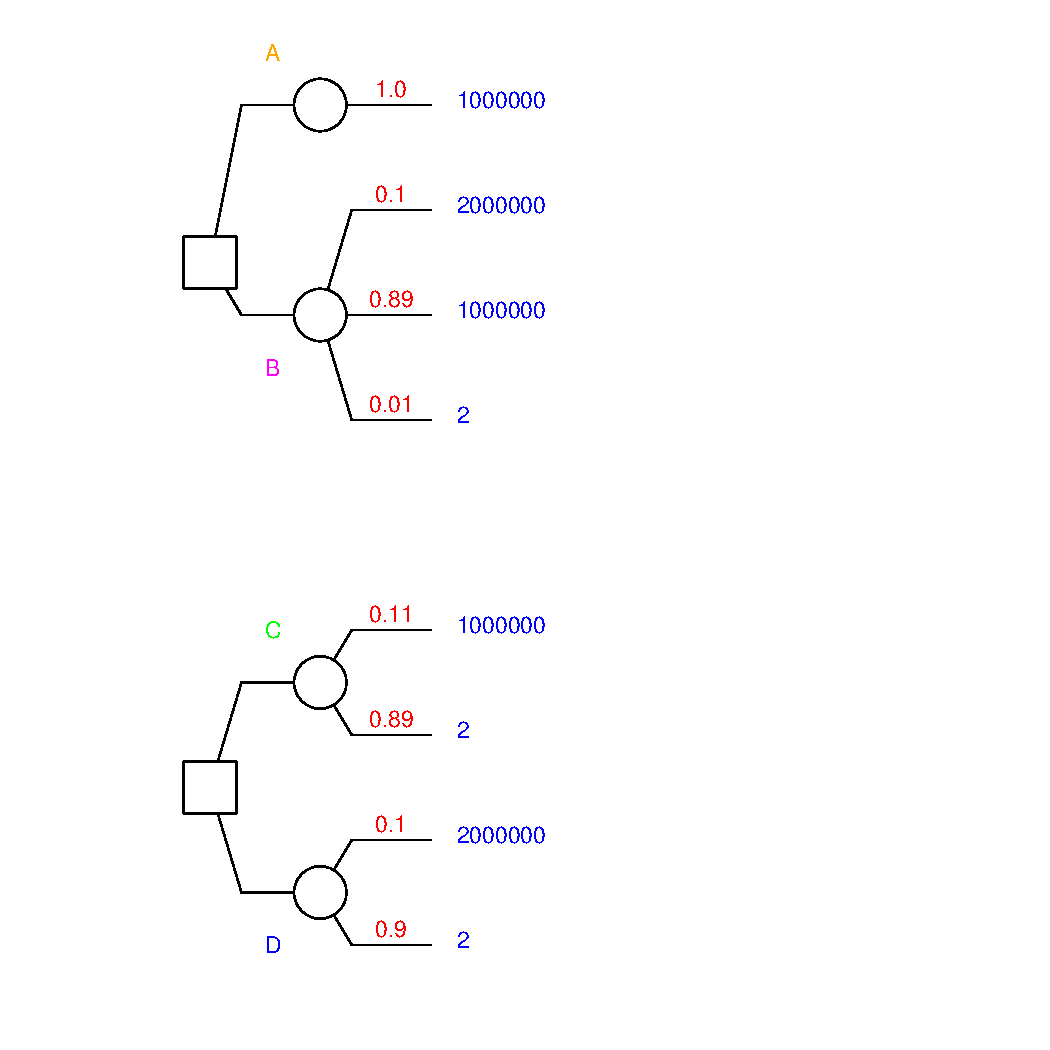
\includegraphics[width=0.8\linewidth]{figure/unnamed-chunk-10} 

}



\end{knitrout}


Now show the simplex.

\begin{knitrout}
\definecolor{shadecolor}{rgb}{0.969, 0.969, 0.969}\color{fgcolor}\begin{kframe}
\begin{alltt}
\hlstd{my_utility} \hlkwb{<-} \hlkwd{Utility}\hlstd{(}\hlkwc{fun}\hlstd{=}\hlstr{"power"}\hlstd{,} \hlkwc{par}\hlstd{=}\hlkwd{c}\hlstd{(}\hlkwc{alpha}\hlstd{=}\hlnum{0.88}\hlstd{,} \hlkwc{beta}\hlstd{=}\hlnum{0.88}\hlstd{,} \hlkwc{lambda}\hlstd{=}\hlnum{2.25}\hlstd{))}

\hlkwd{drawSimplex}\hlstd{(}\hlkwc{x1}\hlstd{=}\hlnum{2}\hlstd{,} \hlkwc{x2}\hlstd{=}\hlnum{1000000}\hlstd{,} \hlkwc{x3}\hlstd{=}\hlnum{2000000}\hlstd{,}
        \hlkwc{line_dot_density}\hlstd{=}\hlnum{1000}\hlstd{,}
        \hlkwc{draw_ev_flag}\hlstd{=}\hlnum{TRUE}\hlstd{,} \hlkwc{ev_colour}\hlstd{=}\hlstr{"black"}\hlstd{,}
        \hlkwc{draw_pt_flag}\hlstd{=}\hlnum{TRUE}\hlstd{,} \hlkwc{alpha}\hlstd{=}\hlnum{0.61}\hlstd{,} \hlkwc{beta}\hlstd{=}\hlnum{0.724}\hlstd{,} \hlkwc{pt_colour}\hlstd{=}\hlstr{"red"}\hlstd{,}
        \hlkwc{draw_utility_flag}\hlstd{=}\hlnum{TRUE}\hlstd{,} \hlkwc{utility}\hlstd{=my_utility,} \hlkwc{eu_colour}\hlstd{=}\hlstr{"purple"}\hlstd{,}
        \hlkwc{start_points}\hlstd{=}\hlkwd{list}\hlstd{(}\hlkwd{c}\hlstd{(}\hlnum{0.1}\hlstd{,}\hlnum{0.9}\hlstd{),}\hlkwd{c}\hlstd{(}\hlnum{0.2}\hlstd{,}\hlnum{0.8}\hlstd{),}\hlkwd{c}\hlstd{(}\hlnum{0.3}\hlstd{,}\hlnum{0.7}\hlstd{),}\hlkwd{c}\hlstd{(}\hlnum{0.4}\hlstd{,}\hlnum{0.6}\hlstd{),}
                \hlkwd{c}\hlstd{(}\hlnum{0.5}\hlstd{,}\hlnum{0.5}\hlstd{),}\hlkwd{c}\hlstd{(}\hlnum{0.6}\hlstd{,}\hlnum{0.4}\hlstd{),}\hlkwd{c}\hlstd{(}\hlnum{0.7}\hlstd{,}\hlnum{0.3}\hlstd{),}\hlkwd{c}\hlstd{(}\hlnum{0.8}\hlstd{,}\hlnum{0.2}\hlstd{),}\hlkwd{c}\hlstd{(}\hlnum{0.9}\hlstd{,}\hlnum{0.1}\hlstd{)),}
        \hlkwc{labels}\hlstd{=}\hlkwd{c}\hlstd{(}\hlstr{"A"}\hlstd{,}\hlstr{"B"}\hlstd{,}\hlstr{"C"}\hlstd{,}\hlstr{"D"}\hlstd{,}\hlstr{"increasing preference"}\hlstd{),}
        \hlkwc{label_positions}\hlstd{=}\hlkwd{list}\hlstd{(}\hlkwd{c}\hlstd{(}\hlnum{0.05}\hlstd{,}\hlnum{0.02}\hlstd{),}\hlkwd{c}\hlstd{(}\hlnum{0.05}\hlstd{,}\hlnum{0.12}\hlstd{),}\hlkwd{c}\hlstd{(}\hlnum{0.92}\hlstd{,}\hlnum{0.02}\hlstd{),}
                \hlkwd{c}\hlstd{(}\hlnum{0.95}\hlstd{,}\hlnum{0.10}\hlstd{),}\hlkwd{c}\hlstd{(}\hlnum{0.7}\hlstd{,}\hlnum{0.7}\hlstd{)),}
        \hlkwc{label_colours}\hlstd{=}\hlkwd{c}\hlstd{(}\hlstr{"orange"}\hlstd{,}\hlstr{"purple"}\hlstd{,}\hlstr{"orange"}\hlstd{,}\hlstr{"purple"}\hlstd{,}\hlstr{"red"}\hlstd{),}
        \hlkwc{label_font_sizes}\hlstd{=}\hlkwd{c}\hlstd{(}\hlnum{12}\hlstd{,}\hlnum{12}\hlstd{,}\hlnum{12}\hlstd{,}\hlnum{12}\hlstd{,}\hlnum{16}\hlstd{),}
        \hlkwc{label_font_faces}\hlstd{=}\hlkwd{c}\hlstd{(}\hlstr{"plain"}\hlstd{,}\hlstr{"plain"}\hlstd{,}\hlstr{"plain"}\hlstd{,}\hlstr{"plain"}\hlstd{,}\hlstr{"bold"}\hlstd{),}
        \hlkwc{label_rotations}\hlstd{=}\hlkwd{c}\hlstd{(}\hlnum{0}\hlstd{,}\hlnum{0}\hlstd{,}\hlnum{0}\hlstd{,}\hlnum{0}\hlstd{,}\hlopt{-}\hlnum{45}\hlstd{),}
        \hlkwc{circle_radii}\hlstd{=}\hlkwd{c}\hlstd{(}\hlnum{0.01}\hlstd{,}\hlnum{0.01}\hlstd{,}\hlnum{0.01}\hlstd{,}\hlnum{0.01}\hlstd{),}
        \hlkwc{circle_outline_colours}\hlstd{=}\hlkwd{c}\hlstd{(}\hlstr{"black"}\hlstd{,}\hlstr{"black"}\hlstd{,}\hlstr{"black"}\hlstd{,}\hlstr{"black"}\hlstd{),}
        \hlkwc{circle_fill_colours}\hlstd{=}\hlkwd{c}\hlstd{(}\hlstr{"orange"}\hlstd{,}\hlstr{"purple"}\hlstd{,}\hlstr{"orange"}\hlstd{,}\hlstr{"purple"}\hlstd{),}
        \hlkwc{circle_positions}\hlstd{=}\hlkwd{list}\hlstd{(}\hlkwd{c}\hlstd{(}\hlnum{0}\hlstd{,}\hlnum{0}\hlstd{),}\hlkwd{c}\hlstd{(}\hlnum{0.01}\hlstd{,}\hlnum{0.1}\hlstd{),}\hlkwd{c}\hlstd{(}\hlnum{0.89}\hlstd{,}\hlnum{0}\hlstd{),}\hlkwd{c}\hlstd{(}\hlnum{0.9}\hlstd{,}\hlnum{0.1}\hlstd{)),}
        \hlkwc{lines}\hlstd{=}\hlkwd{list}\hlstd{(}\hlkwd{c}\hlstd{(}\hlnum{0}\hlstd{,}\hlnum{0}\hlstd{,}\hlnum{0.01}\hlstd{,}\hlnum{0.1}\hlstd{),}\hlkwd{c}\hlstd{(}\hlnum{0.89}\hlstd{,}\hlnum{0}\hlstd{,}\hlnum{0.9}\hlstd{,}\hlnum{0.1}\hlstd{),}
                \hlkwd{c}\hlstd{(}\hlnum{0.01}\hlstd{,}\hlnum{0.1}\hlstd{,}\hlnum{0.9}\hlstd{,}\hlnum{0.1}\hlstd{),}\hlkwd{c}\hlstd{(}\hlnum{0}\hlstd{,}\hlnum{0}\hlstd{,}\hlnum{0.89}\hlstd{,}\hlnum{0}\hlstd{)),}
        \hlkwc{line_widths}\hlstd{=}\hlkwd{c}\hlstd{(}\hlnum{1}\hlstd{,} \hlnum{1}\hlstd{,} \hlnum{1}\hlstd{,} \hlnum{1}\hlstd{),}
        \hlkwc{line_styles}\hlstd{=}\hlkwd{c}\hlstd{(}\hlstr{"dashed"}\hlstd{,} \hlstr{"dashed"}\hlstd{,} \hlstr{"dashed"}\hlstd{,} \hlstr{"dashed"}\hlstd{),}
        \hlkwc{line_colours}\hlstd{=}\hlkwd{c}\hlstd{(}\hlstr{"blue"}\hlstd{,}\hlstr{"blue"}\hlstd{,}\hlstr{"blue"}\hlstd{,}\hlstr{"blue"}\hlstd{),}
        \hlkwc{arrows}\hlstd{=}\hlkwd{list}\hlstd{(}\hlkwd{c}\hlstd{(}\hlnum{0.8}\hlstd{,}\hlnum{0.5}\hlstd{,}\hlnum{0.5}\hlstd{,}\hlnum{0.8}\hlstd{)),}
        \hlkwc{arrow_widths}\hlstd{=}\hlkwd{c}\hlstd{(}\hlnum{2}\hlstd{),} \hlkwc{arrow_styles}\hlstd{=}\hlkwd{c}\hlstd{(}\hlstr{"solid"}\hlstd{),} \hlkwc{arrow_colours}\hlstd{=}\hlkwd{c}\hlstd{(}\hlstr{"red"}\hlstd{))}
\end{alltt}
\end{kframe}

{\centering 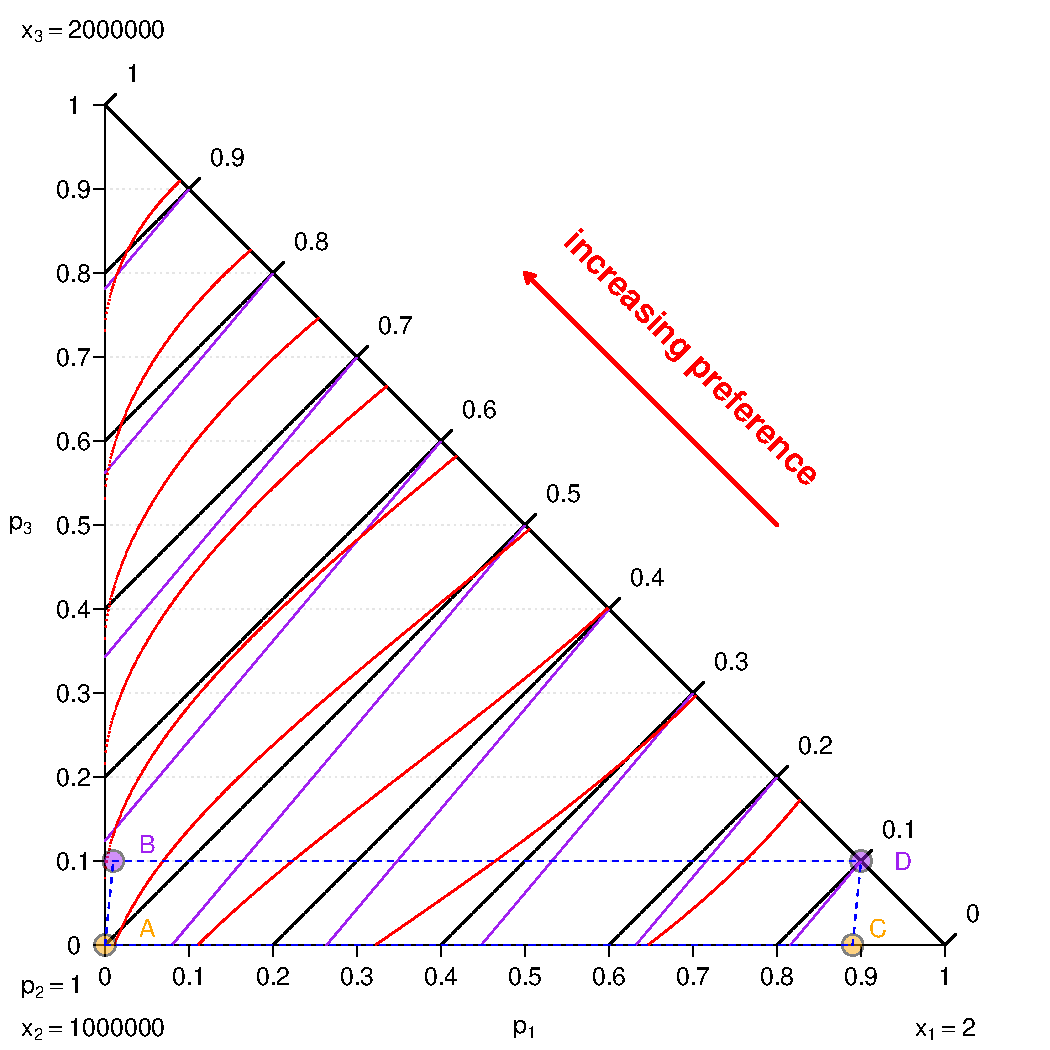
\includegraphics[width=0.8\linewidth]{figure/unnamed-chunk-11} 

}



\end{knitrout}


\subsection{Common ratio paradox}

Create choices problems 3 and 4 from \citet[][p. 266]{Kahneman_Tversky_1979} to illustrate the common ratio paradox.

\begin{knitrout}
\definecolor{shadecolor}{rgb}{0.969, 0.969, 0.969}\color{fgcolor}\begin{kframe}
\begin{alltt}
\hlstd{choice_ids} \hlkwb{<-} \hlkwd{c}\hlstd{(}\hlnum{1}\hlstd{,} \hlnum{1}\hlstd{,} \hlnum{1}\hlstd{,} \hlnum{2}\hlstd{,} \hlnum{2}\hlstd{,} \hlnum{2}\hlstd{,} \hlnum{2}\hlstd{)}
\hlstd{gamble_ids} \hlkwb{<-} \hlkwd{c}\hlstd{(}\hlnum{1}\hlstd{,} \hlnum{1}\hlstd{,} \hlnum{2}\hlstd{,} \hlnum{1}\hlstd{,} \hlnum{1}\hlstd{,} \hlnum{2}\hlstd{,} \hlnum{2}\hlstd{)}
\hlstd{outcome_ids} \hlkwb{<-} \hlkwd{c}\hlstd{(}\hlnum{1}\hlstd{,} \hlnum{1}\hlstd{,} \hlnum{2}\hlstd{,} \hlnum{1}\hlstd{,} \hlnum{2}\hlstd{,} \hlnum{1}\hlstd{,} \hlnum{2}\hlstd{)}
\hlstd{objective_consequences} \hlkwb{<-} \hlkwd{c}\hlstd{(}\hlnum{4000}\hlstd{,} \hlnum{0}\hlstd{,} \hlnum{3000}\hlstd{,}
        \hlnum{4000}\hlstd{,} \hlnum{0}\hlstd{,} \hlnum{3000}\hlstd{,} \hlnum{0}\hlstd{)}
\hlstd{probability_strings} \hlkwb{<-} \hlkwd{c}\hlstd{(}\hlstr{"0.8"}\hlstd{,} \hlstr{"0.2"}\hlstd{,} \hlstr{"1.0"}\hlstd{,}
        \hlstr{"0.2"}\hlstd{,} \hlstr{"0.8"}\hlstd{,} \hlstr{"0.25"}\hlstd{,} \hlstr{"0.75"}\hlstd{)}
\hlstd{my_choices} \hlkwb{<-} \hlkwd{Choices}\hlstd{(}\hlkwc{choice_ids}\hlstd{=choice_ids,}
        \hlkwc{gamble_ids}\hlstd{=gamble_ids,}
        \hlkwc{outcome_ids}\hlstd{=outcome_ids,}
        \hlkwc{objective_consequences}\hlstd{=objective_consequences,}
        \hlkwc{probability_strings}\hlstd{=probability_strings)}
\hlstd{my_choices}
\end{alltt}
\begin{verbatim}
##   cid gid oid   pr   oc
## 1   1   1   1  0.8 4000
## 2   1   1   1  0.2    0
## 3   1   2   2  1.0 3000
## 4   2   1   1  0.2 4000
## 5   2   1   2  0.8    0
## 6   2   2   1 0.25 3000
## 7   2   2   2 0.75    0
\end{verbatim}
\begin{alltt}
\hlkwd{drawChoices}\hlstd{(my_choices,}
        \hlkwc{decision_square_x}\hlstd{=}\hlnum{0.2}\hlstd{,} \hlkwc{decision_square_edge_length}\hlstd{=}\hlnum{0.05}\hlstd{,}
        \hlkwc{circle_radius}\hlstd{=}\hlnum{0.025}\hlstd{,} \hlkwc{y_split_gap}\hlstd{=}\hlnum{0.1}\hlstd{,} \hlkwc{x_split_offset}\hlstd{=}\hlnum{0.03}\hlstd{,}
        \hlkwc{probability_text_digits}\hlstd{=}\hlnum{4}\hlstd{,} \hlkwc{y_probability_text_offset}\hlstd{=}\hlnum{0.015}\hlstd{,}
        \hlkwc{y_value_text_offset}\hlstd{=}\hlnum{0.005}\hlstd{,} \hlkwc{x_value_text_offset}\hlstd{=}\hlnum{0.025}\hlstd{,}
        \hlkwc{probability_text_font_colour}\hlstd{=}\hlstr{"red"}\hlstd{,} \hlkwc{probability_text_font_size}\hlstd{=}\hlnum{11}\hlstd{,}
        \hlkwc{objective_consequence_text_font_colour}\hlstd{=}\hlstr{"blue"}\hlstd{,}
        \hlkwc{objective_consequence_text_font_size}\hlstd{=}\hlnum{11}\hlstd{,} \hlkwc{label}\hlstd{=}\hlkwd{c}\hlstd{(}\hlstr{"A"}\hlstd{,}\hlstr{"B"}\hlstd{,}\hlstr{"C"}\hlstd{,} \hlstr{"D"}\hlstd{),}
        \hlkwc{label_font_colour}\hlstd{=}\hlkwd{c}\hlstd{(}\hlstr{"orange"}\hlstd{,}\hlstr{"magenta"}\hlstd{,}\hlstr{"green"}\hlstd{,}\hlstr{"blue"}\hlstd{),}
        \hlkwc{label_font_size}\hlstd{=}\hlkwd{c}\hlstd{(}\hlnum{11}\hlstd{,}\hlnum{11}\hlstd{,}\hlnum{11}\hlstd{,}\hlnum{11}\hlstd{),}
        \hlkwc{label_positions}\hlstd{=}\hlkwd{list}\hlstd{(}\hlkwd{c}\hlstd{(}\hlnum{0.26}\hlstd{,}\hlnum{0.85}\hlstd{),}\hlkwd{c}\hlstd{(}\hlnum{0.26}\hlstd{,}\hlnum{0.6}\hlstd{),}
                \hlkwd{c}\hlstd{(}\hlnum{0.26}\hlstd{,}\hlnum{0.4}\hlstd{),}\hlkwd{c}\hlstd{(}\hlnum{0.26}\hlstd{,}\hlnum{0.1}\hlstd{)))}
\end{alltt}
\end{kframe}

{\centering 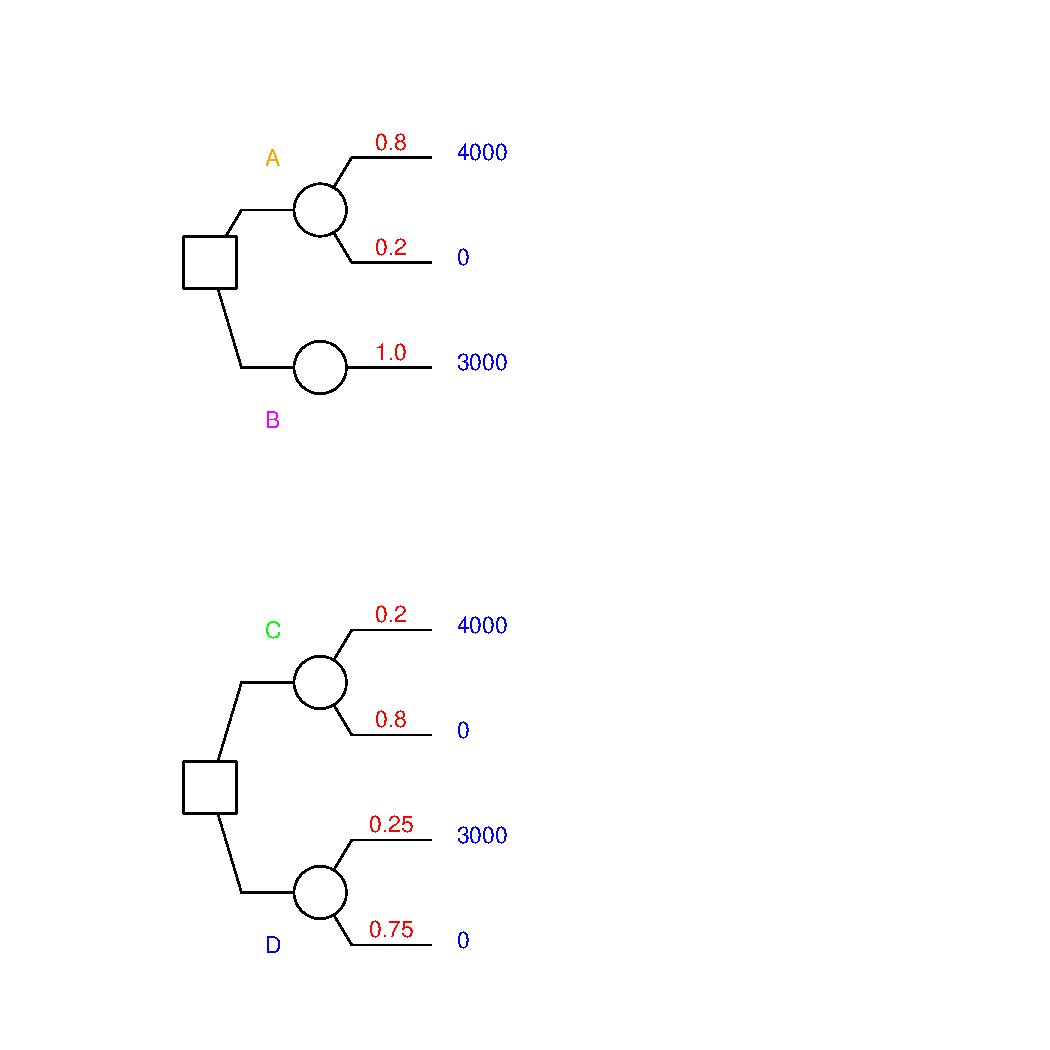
\includegraphics[width=0.8\linewidth]{figure/unnamed-chunk-12} 

}



\end{knitrout}


In a sample of $95$ people, $80\%$ preferred $B > A$ and $65\%$ preferred $C > D$.
EU predicts either the preferences $A > B$ and $C > D$ or the preferences $B > A$ and $D > C$.
Following the reasoning of the previous common consequence example,
if decision makers are preferring $B > A$, this implies (again applying the expected utility formula of Eq. \eqref{eu_equation}) that

\begin{equation}
\begin{split}
EU(B) &> EU(A)\\
1.0 \times u(3000) &> 0.8 \times u(4000) + 0.2 \times u(0)\\
\frac{u(3000)}{u(4000)} &> 0.8 \times + \frac{0.2 \times u(0)}{u(4000)}\\
\frac{u(3000)}{u(4000)} &> 0.8,
\end{split}
\end{equation}

dividing both sides of the inequality by $u(4000)$ and setting $u(0) = 0$. If decision makers are preferring $C > D$, this implies that

\begin{equation}
\begin{split}
EU(C) &> EU(D)\\
0.2 \times u(4000) + 0.8 \times u(0) &> 0.25 \times u(3000) + 0.75 \times u(0)\\
0.2 + \frac{0.8 \times u(0)}{u(4000)} &> \frac{0.25 \times u(3000)}{u(4000)} + \frac{0.75 \times u(0)}{u(4000)}\\
0.2 &> \frac{0.25 \times u(3000)}{u(4000)}\\
0.8 &> \frac{u(3000)}{u(4000)}.
\end{split}
\end{equation}

The inequalities are reversed across the two choice situations. Expected utility predicts that people will either choose $A > B$ and $C > D$ or choose $B > A$ and $D > C$ if the independence axiom holds. It does not predict the empirically observed pattern. {\bf pt} can be used to show the comparative theoretical predictions of all the decision making theories implemented in the package. Firstly show the EV.

\begin{knitrout}
\definecolor{shadecolor}{rgb}{0.969, 0.969, 0.969}\color{fgcolor}\begin{kframe}
\begin{alltt}
\hlkwd{compareEV}\hlstd{(my_choices,} \hlkwc{digits}\hlstd{=}\hlnum{4}\hlstd{)}
\end{alltt}
\begin{verbatim}
##   cid gid   ev
## 1   1   1 3200
## 2   1   2 3000
## 3   2   1  800
## 4   2   2  750
\end{verbatim}
\end{kframe}
\end{knitrout}


Gambles A and C have the highest expected values. However, they are also the riskier choices.
Compute the EU with a hypothetical concave utility function, and show the risk premium.

\begin{knitrout}
\definecolor{shadecolor}{rgb}{0.969, 0.969, 0.969}\color{fgcolor}\begin{kframe}
\begin{alltt}
\hlstd{my_utility} \hlkwb{<-} \hlkwd{Utility}\hlstd{(}\hlkwc{fun}\hlstd{=}\hlstr{"power"}\hlstd{,} \hlkwc{par}\hlstd{=}\hlkwd{c}\hlstd{(}\hlkwc{alpha}\hlstd{=}\hlnum{0.88}\hlstd{,} \hlkwc{beta}\hlstd{=}\hlnum{0.88}\hlstd{,} \hlkwc{lambda}\hlstd{=}\hlnum{1}\hlstd{))}
\hlstd{eu_df} \hlkwb{<-} \hlkwd{compareEU}\hlstd{(my_choices,} \hlkwc{utility}\hlstd{=my_utility,} \hlkwc{digits}\hlstd{=}\hlnum{4}\hlstd{)}
\hlstd{eu_df}
\end{alltt}
\begin{verbatim}
##   cid gid   ev    eu    ce                 rp
## 1   1   1 3200  1183  3104              95.91
## 2   1   2 3000  1148  3000 -0.000000000001819
## 3   2   1  800 295.7 642.4              157.6
## 4   2   2  750   287 620.8              129.2
\end{verbatim}
\begin{alltt}
\hlstd{ev} \hlkwb{<-} \hlkwd{as.numeric}\hlstd{(eu_df}\hlopt{$}\hlstd{ev[}\hlnum{1}\hlstd{])}
\hlstd{eu} \hlkwb{<-} \hlkwd{as.numeric}\hlstd{(eu_df}\hlopt{$}\hlstd{eu[}\hlnum{1}\hlstd{])}
\hlstd{ce} \hlkwb{<-} \hlkwd{as.numeric}\hlstd{(eu_df}\hlopt{$}\hlstd{ce[}\hlnum{1}\hlstd{])}
\hlkwd{plotRP}\hlstd{(}\hlkwc{my_title} \hlstd{=} \hlstr{"risk premium"}\hlstd{,}
        \hlkwc{my_title_colour}\hlstd{=}\hlstr{"black"}\hlstd{,} \hlkwc{my_title_font_size}\hlstd{=}\hlnum{4}\hlstd{,}
        \hlkwc{my_x_label} \hlstd{=} \hlstr{"objective consequence"}\hlstd{,}
        \hlkwc{my_y_label} \hlstd{=} \hlstr{"subjective value"}\hlstd{,} \hlkwc{xmin} \hlstd{=} \hlnum{2500}\hlstd{,} \hlkwc{xmax} \hlstd{=} \hlnum{3500}\hlstd{,}
        \hlkwc{my_color}\hlstd{=}\hlstr{"violet"}\hlstd{,}
        \hlkwc{fun}\hlstd{=power_uf,}
        \hlkwc{par}\hlstd{=}\hlkwd{c}\hlstd{(}\hlkwc{alpha}\hlstd{=}\hlnum{0.88}\hlstd{,} \hlkwc{beta}\hlstd{=}\hlnum{0.88}\hlstd{,} \hlkwc{lambda}\hlstd{=}\hlnum{1}\hlstd{),}
        \hlkwc{ev}\hlstd{=ev,} \hlkwc{eu}\hlstd{=eu,} \hlkwc{ce}\hlstd{=ce,}
        \hlkwc{my_labels}\hlstd{=}\hlkwd{c}\hlstd{(}\hlkwd{expression}\hlstd{(}\hlkwd{paste}\hlstd{(}\hlkwd{U}\hlstd{(x)}\hlopt{==}\hlstd{x}\hlopt{^}\hlstd{alpha,} \hlstr{",     "}\hlstd{, x}\hlopt{>=}\hlnum{0}\hlstd{)),}
                \hlkwd{expression}\hlstd{(}\hlkwd{paste}\hlstd{(}\hlkwd{plain}\hlstd{()}\hlopt{==-}\hlstd{lambda} \hlopt{*} \hlstd{(}\hlopt{-}\hlstd{x)}\hlopt{^}\hlstd{beta,} \hlstr{", "}\hlstd{, x}\hlopt{<}\hlnum{0}\hlstd{)),}
                \hlstr{"ev"}\hlstd{,}\hlstr{"eu"}\hlstd{,}\hlstr{"ce"}\hlstd{,}\hlstr{"rp"}\hlstd{),}
        \hlkwc{my_label_colors}\hlstd{=}\hlkwd{c}\hlstd{(}\hlstr{"violet"}\hlstd{,}\hlstr{"violet"}\hlstd{,}\hlstr{"black"}\hlstd{,}\hlstr{"red"}\hlstd{,}\hlstr{"orange"}\hlstd{,}\hlstr{"blue"}\hlstd{),}
        \hlkwc{my_label_positions}\hlstd{=}\hlkwd{list}\hlstd{(}\hlkwd{c}\hlstd{(}\hlnum{2700}\hlstd{,}\hlnum{1275}\hlstd{),}\hlkwd{c}\hlstd{(}\hlnum{2740}\hlstd{,}\hlnum{1250}\hlstd{),}\hlkwd{c}\hlstd{(}\hlnum{3250}\hlstd{,}\hlnum{1075}\hlstd{),}
                \hlkwd{c}\hlstd{(}\hlnum{2800}\hlstd{,}\hlnum{1170}\hlstd{),}\hlkwd{c}\hlstd{(}\hlnum{3050}\hlstd{,}\hlnum{1075}\hlstd{),}\hlkwd{c}\hlstd{(}\hlnum{3150}\hlstd{,}\hlnum{1170}\hlstd{)),}
        \hlkwc{font_scaling}\hlstd{=}\hlnum{1}\hlstd{)}
\end{alltt}
\end{kframe}

{\centering 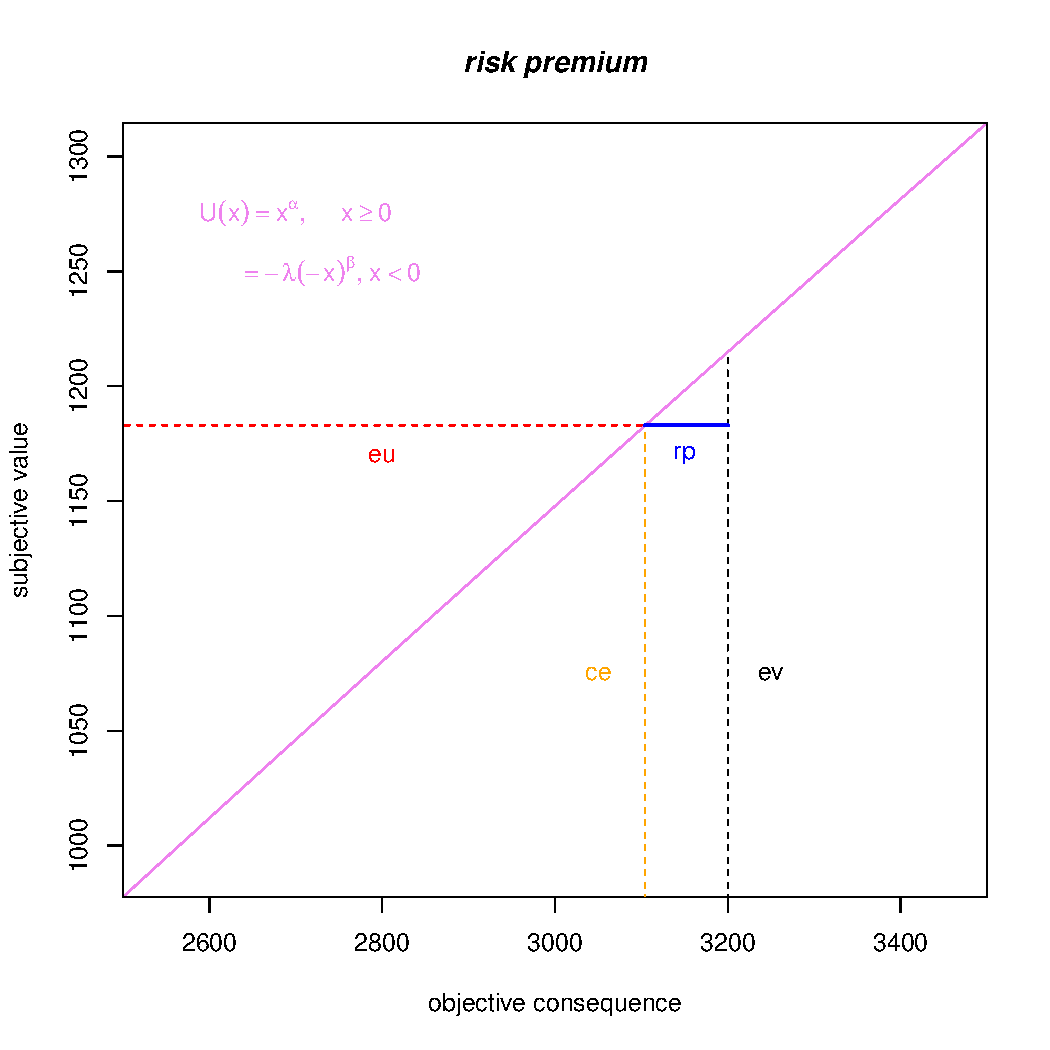
\includegraphics[width=0.8\linewidth]{figure/unnamed-chunk-14} 

}



\end{knitrout}


For this parameterisation $A > B$ and $C > D$. {\bf pt} can be used to perform a sensitivity analysis to determine
critical values for risk tolerances.
The parameters for which the EU preferences are reversed so that $B > A$ and $D > C$ can be identified using
the code below. Note that both these parameterisations use concave utility functions.

\begin{knitrout}
\definecolor{shadecolor}{rgb}{0.969, 0.969, 0.969}\color{fgcolor}\begin{kframe}
\begin{alltt}
\hlstd{my_utility} \hlkwb{<-} \hlkwd{Utility}\hlstd{(}\hlkwc{fun}\hlstd{=}\hlstr{"power"}\hlstd{,} \hlkwc{par}\hlstd{=}\hlkwd{c}\hlstd{(}\hlkwc{alpha}\hlstd{=}\hlnum{0.78}\hlstd{,} \hlkwc{beta}\hlstd{=}\hlnum{0.78}\hlstd{,} \hlkwc{lambda}\hlstd{=}\hlnum{1}\hlstd{))}
\hlkwd{compareEU}\hlstd{(my_choices,} \hlkwc{utility}\hlstd{=my_utility,} \hlkwc{digits}\hlstd{=}\hlnum{4}\hlstd{)}
\end{alltt}
\begin{verbatim}
##   cid gid   ev    eu    ce                rp
## 1   1   1 3200 516.1  3005             195.2
## 2   1   2 3000 515.4  3000 0.000000000001364
## 3   2   1  800   129 508.1             291.9
## 4   2   2  750 128.9 507.3             242.7
\end{verbatim}
\end{kframe}
\end{knitrout}


\begin{knitrout}
\definecolor{shadecolor}{rgb}{0.969, 0.969, 0.969}\color{fgcolor}\begin{kframe}
\begin{alltt}
\hlstd{my_utility} \hlkwb{<-} \hlkwd{Utility}\hlstd{(}\hlkwc{fun}\hlstd{=}\hlstr{"power"}\hlstd{,} \hlkwc{par}\hlstd{=}\hlkwd{c}\hlstd{(}\hlkwc{alpha}\hlstd{=}\hlnum{0.77}\hlstd{,} \hlkwc{beta}\hlstd{=}\hlnum{0.78}\hlstd{,} \hlkwc{lambda}\hlstd{=}\hlnum{1}\hlstd{))}
\hlkwd{compareEU}\hlstd{(my_choices,} \hlkwc{utility}\hlstd{=my_utility,} \hlkwc{digits}\hlstd{=}\hlnum{4}\hlstd{)}
\end{alltt}
\begin{verbatim}
##   cid gid   ev    eu    ce    rp
## 1   1   1 3200   475  2994 206.3
## 2   1   2 3000 475.8  3000     0
## 3   2   1  800 118.7 494.7 305.3
## 4   2   2  750 118.9 495.7 254.3
\end{verbatim}
\end{kframe}
\end{knitrout}


Note the reversal in preferences. Using a linear utility function $u(x) = x$ gives the same result as EV.

\begin{knitrout}
\definecolor{shadecolor}{rgb}{0.969, 0.969, 0.969}\color{fgcolor}\begin{kframe}
\begin{alltt}
\hlstd{my_utility} \hlkwb{<-} \hlkwd{Utility}\hlstd{(}\hlkwc{fun}\hlstd{=}\hlstr{"power"}\hlstd{,} \hlkwc{par}\hlstd{=}\hlkwd{c}\hlstd{(}\hlkwc{alpha}\hlstd{=}\hlnum{1}\hlstd{,} \hlkwc{beta}\hlstd{=}\hlnum{1}\hlstd{,} \hlkwc{lambda}\hlstd{=}\hlnum{1}\hlstd{))}
\hlkwd{compareEU}\hlstd{(my_choices,} \hlkwc{utility}\hlstd{=my_utility,} \hlkwc{digits}\hlstd{=}\hlnum{4}\hlstd{)}
\end{alltt}
\begin{verbatim}
##   cid gid   ev   eu   ce rp
## 1   1   1 3200 3200 3200  0
## 2   1   2 3000 3000 3000  0
## 3   2   1  800  800  800  0
## 4   2   2  750  750  750  0
\end{verbatim}
\end{kframe}
\end{knitrout}


Compute the predictions for RDU.

\begin{knitrout}
\definecolor{shadecolor}{rgb}{0.969, 0.969, 0.969}\color{fgcolor}\begin{kframe}
\begin{alltt}
\hlstd{tk_1992_utility} \hlkwb{<-} \hlkwd{Utility}\hlstd{(}\hlkwc{fun}\hlstd{=}\hlstr{"power"}\hlstd{,} \hlkwc{par}\hlstd{=}\hlkwd{c}\hlstd{(}\hlkwc{alpha}\hlstd{=}\hlnum{0.88}\hlstd{,} \hlkwc{beta}\hlstd{=}\hlnum{0.88}\hlstd{,} \hlkwc{lambda}\hlstd{=}\hlnum{2.25}\hlstd{))}
\hlstd{tk_1992_positive_prob_weight} \hlkwb{<-} \hlkwd{ProbWeight}\hlstd{(}\hlkwc{fun}\hlstd{=}\hlstr{"Tversky_Kahneman_1992"}\hlstd{,} \hlkwc{par}\hlstd{=}\hlkwd{c}\hlstd{(}\hlkwc{alpha}\hlstd{=}\hlnum{0.61}\hlstd{))}
\hlkwd{compareRDU}\hlstd{(my_choices,} \hlkwc{prob_weight}\hlstd{=tk_1992_positive_prob_weight,} \hlkwc{utility}\hlstd{=tk_1992_utility,} \hlkwc{digits}\hlstd{=}\hlnum{4}\hlstd{)}
\end{alltt}
\begin{verbatim}
##   cid gid   ev   rdu    ce                 rp
## 1   1   1 3200 898.1  2270              929.9
## 2   1   2 3000  1148  3000 -0.000000000001819
## 3   2   1  800 385.5 868.4             -68.37
## 4   2   2  750 333.7   737              12.99
\end{verbatim}
\end{kframe}
\end{knitrout}


In contrast, RDU predicts the preferences $B > A$ and $C > D$. PT reduces to RDU if all outcomes are strictly positive so its predictions are identical to RDU.

\begin{knitrout}
\definecolor{shadecolor}{rgb}{0.969, 0.969, 0.969}\color{fgcolor}\begin{kframe}
\begin{alltt}
\hlstd{tk_1992_utility} \hlkwb{<-} \hlkwd{Utility}\hlstd{(}\hlkwc{fun}\hlstd{=}\hlstr{"power"}\hlstd{,} \hlkwc{par}\hlstd{=}\hlkwd{c}\hlstd{(}\hlkwc{alpha}\hlstd{=}\hlnum{0.88}\hlstd{,} \hlkwc{beta}\hlstd{=}\hlnum{0.88}\hlstd{,} \hlkwc{lambda}\hlstd{=}\hlnum{2.25}\hlstd{))}
\hlstd{tk_1992_positive_prob_weight} \hlkwb{<-} \hlkwd{ProbWeight}\hlstd{(}\hlkwc{fun}\hlstd{=}\hlstr{"Tversky_Kahneman_1992"}\hlstd{,} \hlkwc{par}\hlstd{=}\hlkwd{c}\hlstd{(}\hlkwc{alpha}\hlstd{=}\hlnum{0.61}\hlstd{))}
\hlstd{tk_1992_negative_prob_weight} \hlkwb{<-} \hlkwd{ProbWeight}\hlstd{(}\hlkwc{fun}\hlstd{=}\hlstr{"Tversky_Kahneman_1992"}\hlstd{,} \hlkwc{par}\hlstd{=}\hlkwd{c}\hlstd{(}\hlkwc{alpha}\hlstd{=}\hlnum{0.69}\hlstd{))}
\hlkwd{comparePT}\hlstd{(my_choices,}
        \hlkwc{prob_weight_for_positive_outcomes}\hlstd{=tk_1992_positive_prob_weight,}
        \hlkwc{prob_weight_for_negative_outcomes}\hlstd{=tk_1992_negative_prob_weight,}
        \hlkwc{utility}\hlstd{=tk_1992_utility,} \hlkwc{digits}\hlstd{=}\hlnum{4}\hlstd{)}
\end{alltt}
\begin{verbatim}
##   cid gid   ev    pt    ce                 rp
## 1   1   1 3200 898.1  2270              929.9
## 2   1   2 3000  1148  3000 -0.000000000001819
## 3   2   1  800 385.5 868.4             -68.37
## 4   2   2  750 333.7   737              12.99
\end{verbatim}
\end{kframe}
\end{knitrout}


PT explains the common ratio paradox using a curved probability weighting function. This can be depicted using {\bf pt}.

\begin{knitrout}
\definecolor{shadecolor}{rgb}{0.969, 0.969, 0.969}\color{fgcolor}\begin{kframe}
\begin{alltt}
\hlkwd{plotProbW}\hlstd{(}\hlkwc{my_title}\hlstd{=}\hlkwd{expression}\hlstd{(}\hlkwd{paste}\hlstd{(}\hlstr{"Tversky & Kahneman (1992), "}\hlstd{,}
        \hlstd{alpha}\hlopt{==}\hlnum{0.61}\hlstd{)),}
        \hlkwc{my_title_colour}\hlstd{=}\hlstr{"black"}\hlstd{,} \hlkwc{my_title_font_size}\hlstd{=}\hlnum{4}\hlstd{,}
        \hlkwc{my_x_label} \hlstd{=} \hlstr{"p"}\hlstd{,} \hlkwc{my_y_label} \hlstd{=} \hlstr{"w(p)"}\hlstd{,}
        \hlkwc{pwf}\hlstd{=kt_pwf,} \hlkwc{par}\hlstd{=}\hlkwd{c}\hlstd{(}\hlkwc{alpha}\hlstd{=}\hlnum{0.61}\hlstd{),}
        \hlkwc{draw_reference_line_flag}\hlstd{=}\hlnum{TRUE}\hlstd{,} \hlkwc{reference_line_colour}\hlstd{=}\hlstr{"red"}\hlstd{,}
        \hlkwc{reference_line_style}\hlstd{=}\hlstr{"dotted"}\hlstd{,}
        \hlkwc{my_labels}\hlstd{=}\hlkwd{c}\hlstd{(}\hlkwd{expression}\hlstd{(}\hlkwd{paste}\hlstd{(}\hlkwd{w}\hlstd{(}\hlkwd{italic}\hlstd{(p))} \hlopt{==} \hlkwd{frac}\hlstd{(}\hlkwd{italic}\hlstd{(p)}\hlopt{^}\hlstd{alpha,}
                \hlstd{(}\hlkwd{italic}\hlstd{(p)}\hlopt{^}\hlstd{alpha} \hlopt{+} \hlstd{(}\hlnum{1}\hlopt{-}\hlkwd{italic}\hlstd{(p))}\hlopt{^}\hlstd{alpha)}\hlopt{^}\hlstd{(}\hlnum{1}\hlopt{/}\hlstd{alpha))))),}
        \hlkwc{my_label_positions}\hlstd{=}\hlkwd{list}\hlstd{(}\hlkwd{c}\hlstd{(}\hlnum{0.4}\hlstd{,}\hlnum{0.8}\hlstd{)),}
        \hlkwc{font_scaling}\hlstd{=}\hlnum{1.0}\hlstd{)}
\end{alltt}
\end{kframe}

{\centering 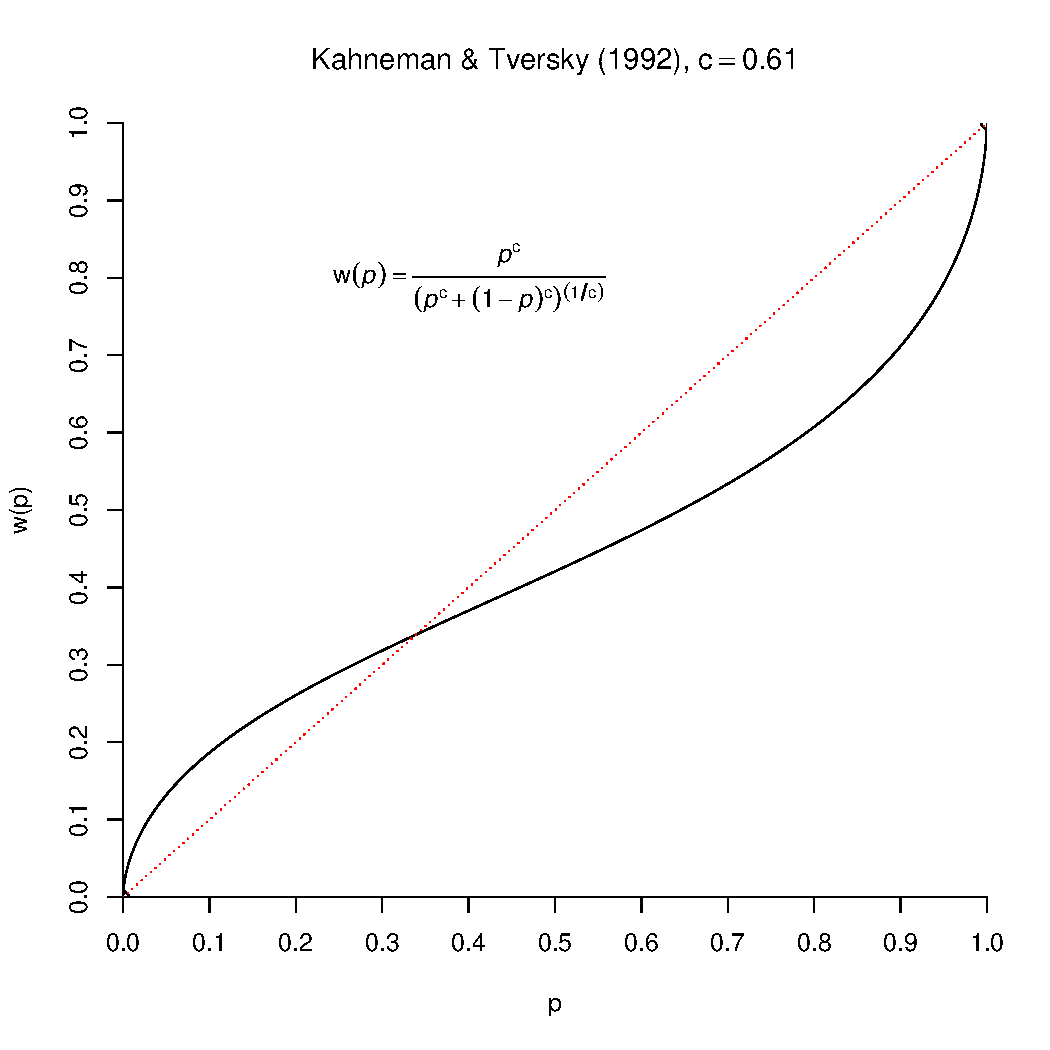
\includegraphics[width=\maxwidth]{figure/unnamed-chunk-20} 

}



\end{knitrout}


This function is only strictly increasing for $\alpha \geq 0.28$. A family of
$\alpha$ values can be plotted (see e.g. \cite[][p. 207 Figure 7.2.1]{Wakker_2010}). The lower the $\alpha$ parameter, the more the decision maker exhibits likelihood insensitivity.

\begin{knitrout}
\definecolor{shadecolor}{rgb}{0.969, 0.969, 0.969}\color{fgcolor}\begin{kframe}
\begin{alltt}
\hlkwd{plotOneParProbWFam}\hlstd{(}\hlkwc{my_title}\hlstd{=}\hlstr{"Tversky & Kahneman (1992) family"}\hlstd{,}
        \hlkwc{my_title_colour}\hlstd{=}\hlstr{"black"}\hlstd{,} \hlkwc{my_title_font_size}\hlstd{=}\hlnum{4}\hlstd{,}
        \hlkwc{my_x_label} \hlstd{=} \hlstr{"p"}\hlstd{,} \hlkwc{my_y_label} \hlstd{=} \hlstr{"w(p)"}\hlstd{,} \hlkwc{pwf}\hlstd{=kt_pwf,}
        \hlkwc{par}\hlstd{=}\hlkwd{c}\hlstd{(}\hlnum{0.3}\hlstd{,} \hlnum{0.61}\hlstd{,} \hlnum{0.8}\hlstd{,} \hlnum{1.0}\hlstd{,} \hlnum{1.3}\hlstd{),}
        \hlkwc{draw_reference_line_flag}\hlstd{=}\hlnum{TRUE}\hlstd{,} \hlkwc{reference_line_colour}\hlstd{=}\hlstr{"red"}\hlstd{,}
        \hlkwc{reference_line_style}\hlstd{=}\hlstr{"dotted"}\hlstd{,}
        \hlkwc{my_labels}\hlstd{=}\hlkwd{c}\hlstd{(}\hlkwd{expression}\hlstd{(}\hlkwd{paste}\hlstd{(alpha} \hlopt{==} \hlnum{0.3}\hlstd{)),}
        \hlkwd{expression}\hlstd{(}\hlkwd{paste}\hlstd{(alpha} \hlopt{==} \hlnum{0.61}\hlstd{)),}
        \hlkwd{expression}\hlstd{(}\hlkwd{paste}\hlstd{(alpha} \hlopt{==} \hlnum{0.8}\hlstd{)),}
        \hlkwd{expression}\hlstd{(}\hlkwd{paste}\hlstd{(alpha} \hlopt{==} \hlnum{1.0}\hlstd{)),}
        \hlkwd{expression}\hlstd{(}\hlkwd{paste}\hlstd{(alpha} \hlopt{==} \hlnum{1.3}\hlstd{)),}
        \hlkwd{expression}\hlstd{(}\hlkwd{paste}\hlstd{(}\hlkwd{w}\hlstd{(}\hlkwd{italic}\hlstd{(p))} \hlopt{==} \hlkwd{frac}\hlstd{(}\hlkwd{italic}\hlstd{(p)}\hlopt{^}\hlstd{alpha,}
        \hlstd{(}\hlkwd{italic}\hlstd{(p)}\hlopt{^}\hlstd{alpha} \hlopt{+} \hlstd{(}\hlnum{1}\hlopt{-}\hlkwd{italic}\hlstd{(p))}\hlopt{^}\hlstd{alpha)}\hlopt{^}\hlstd{(}\hlnum{1}\hlopt{/}\hlstd{alpha))))),}
        \hlkwc{my_label_positions}\hlstd{=}\hlkwd{list}\hlstd{(}\hlkwd{c}\hlstd{(}\hlnum{0.9}\hlstd{,}\hlnum{0.15}\hlstd{),}\hlkwd{c}\hlstd{(}\hlnum{0.7}\hlstd{,}\hlnum{0.45}\hlstd{),}\hlkwd{c}\hlstd{(}\hlnum{0.15}\hlstd{,}\hlnum{0.5}\hlstd{),}
        \hlkwd{c}\hlstd{(}\hlnum{0.31}\hlstd{,}\hlnum{0.62}\hlstd{),}\hlkwd{c}\hlstd{(}\hlnum{0.5}\hlstd{,}\hlnum{0.7}\hlstd{),}\hlkwd{c}\hlstd{(}\hlnum{0.42}\hlstd{,} \hlnum{0.9}\hlstd{)),}
        \hlkwc{font_scaling}\hlstd{=}\hlnum{1.0}\hlstd{,}
        \hlkwc{arrow_positions} \hlstd{=} \hlkwd{list}\hlstd{(}\hlkwd{c}\hlstd{(}\hlnum{0.3}\hlstd{,}\hlnum{0.5}\hlstd{,}\hlnum{0.39}\hlstd{,}\hlnum{0.41}\hlstd{),}\hlkwd{c}\hlstd{(}\hlnum{0.42}\hlstd{,}\hlnum{0.58}\hlstd{,}\hlnum{0.52}\hlstd{,}\hlnum{0.51}\hlstd{),}
                \hlkwd{c}\hlstd{(}\hlnum{0.59}\hlstd{,}\hlnum{0.66}\hlstd{,}\hlnum{0.66}\hlstd{,}\hlnum{0.66}\hlstd{)))}
\end{alltt}
\end{kframe}

{\centering 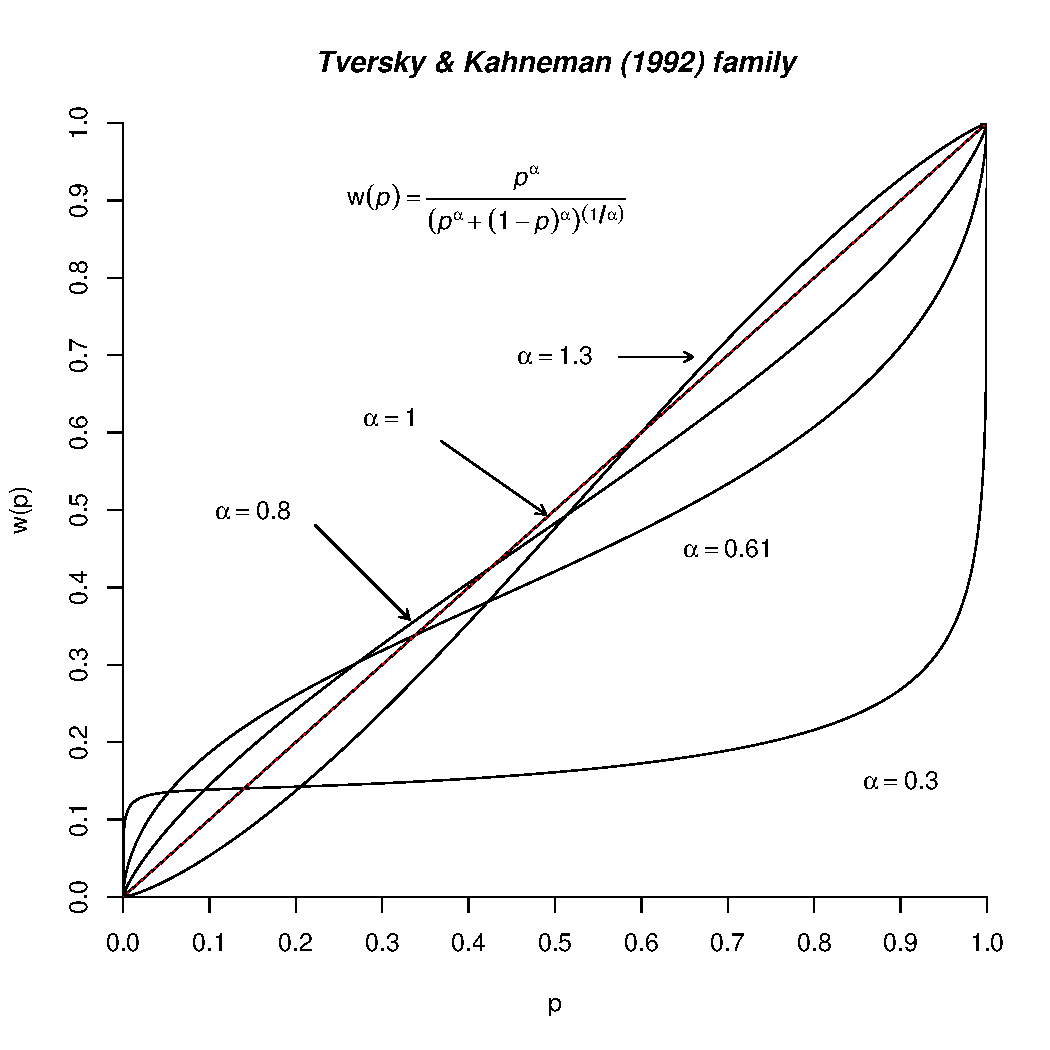
\includegraphics[width=\maxwidth]{figure/unnamed-chunk-21} 

}



\end{knitrout}


Rather than use the single parameter probability weighting functional form of \cite{Tversky_Kahneman_1992}, \cite{Gonzalez_Wu_1999} have proposed the use of
a two-parameter ``linear in log odds" probability weighting function to model probability discriminability and gamble attractiveness \cite[Figure 4 p. 140]{Gonzalez_Wu_1999}. The parameter $\gamma$ controls curvature and $\delta$ controls elevation. {\bf pt} can be used to show the effects of varying $\delta$ on the elevation. Lower values of $\delta$ decrease the elevation.

\begin{knitrout}
\definecolor{shadecolor}{rgb}{0.969, 0.969, 0.969}\color{fgcolor}\begin{kframe}
\begin{alltt}
\hlkwd{plotTwoParProbWFam}\hlstd{(}\hlkwc{my_title}\hlstd{=}\hlkwd{expression}\hlstd{(}\hlkwd{paste}\hlstd{(}\hlstr{"linear in log odds,  "}\hlstd{,}
        \hlstd{gamma} \hlopt{==} \hlnum{0.6}\hlstd{)),}
        \hlkwc{my_title_colour}\hlstd{=}\hlstr{"black"}\hlstd{,} \hlkwc{my_title_font_size}\hlstd{=}\hlnum{4}\hlstd{,}
        \hlkwc{my_x_label} \hlstd{=} \hlstr{"p"}\hlstd{,} \hlkwc{my_y_label} \hlstd{=} \hlstr{"w(p)"}\hlstd{,} \hlkwc{pwf}\hlstd{=linear_in_log_odds_pwf,}
        \hlkwc{par}\hlstd{=}\hlkwd{list}\hlstd{(}\hlkwc{a_list}\hlstd{=}\hlkwd{c}\hlstd{(}\hlnum{0.6}\hlstd{),} \hlkwc{b_list}\hlstd{=}\hlkwd{seq}\hlstd{(}\hlkwc{from}\hlstd{=}\hlnum{0.2}\hlstd{,} \hlkwc{to}\hlstd{=}\hlnum{1.8}\hlstd{,} \hlkwc{by}\hlstd{=}\hlnum{0.06}\hlstd{)),}
        \hlkwc{draw_reference_line_flag}\hlstd{=}\hlnum{TRUE}\hlstd{,} \hlkwc{reference_line_colour}\hlstd{=}\hlstr{"red"}\hlstd{,}
        \hlkwc{reference_line_style}\hlstd{=}\hlstr{"dotted"}\hlstd{,}
        \hlkwc{my_labels}\hlstd{=}\hlkwd{c}\hlstd{(}\hlkwd{expression}\hlstd{(}\hlkwd{paste}\hlstd{(delta} \hlopt{==} \hlnum{0.2}\hlstd{)),}
                \hlkwd{expression}\hlstd{(}\hlkwd{paste}\hlstd{(delta} \hlopt{==} \hlnum{1.8}\hlstd{)),}
                \hlkwd{expression}\hlstd{(}\hlkwd{paste}\hlstd{(}\hlkwd{w}\hlstd{(}\hlkwd{italic}\hlstd{(p))} \hlopt{==} \hlkwd{frac}\hlstd{(delta} \hlopt{*} \hlkwd{italic}\hlstd{(p)}\hlopt{^}\hlstd{gamma,}
                        \hlstd{delta} \hlopt{*} \hlkwd{italic}\hlstd{(p)}\hlopt{^}\hlstd{gamma} \hlopt{+} \hlstd{(}\hlnum{1}\hlopt{-}\hlkwd{italic}\hlstd{(p))}\hlopt{^}\hlstd{gamma)))),}
        \hlkwc{my_label_positions}\hlstd{=}\hlkwd{list}\hlstd{(}\hlkwd{c}\hlstd{(}\hlnum{0.7}\hlstd{,}\hlnum{0.09}\hlstd{),}\hlkwd{c}\hlstd{(}\hlnum{0.2}\hlstd{,}\hlnum{0.6}\hlstd{),}\hlkwd{c}\hlstd{(}\hlnum{0.42}\hlstd{,} \hlnum{0.9}\hlstd{)),}
        \hlkwc{font_scaling}\hlstd{=}\hlnum{1.0}\hlstd{,}
        \hlkwc{arrow_positions} \hlstd{=} \hlkwd{list}\hlstd{(}\hlkwd{c}\hlstd{(}\hlnum{0.28}\hlstd{,}\hlnum{0.56}\hlstd{,}\hlnum{0.35}\hlstd{,}\hlnum{0.53}\hlstd{),}\hlkwd{c}\hlstd{(}\hlnum{0.7}\hlstd{,}\hlnum{0.23}\hlstd{,}\hlnum{0.75}\hlstd{,}\hlnum{0.35}\hlstd{)))}
\end{alltt}
\end{kframe}

{\centering 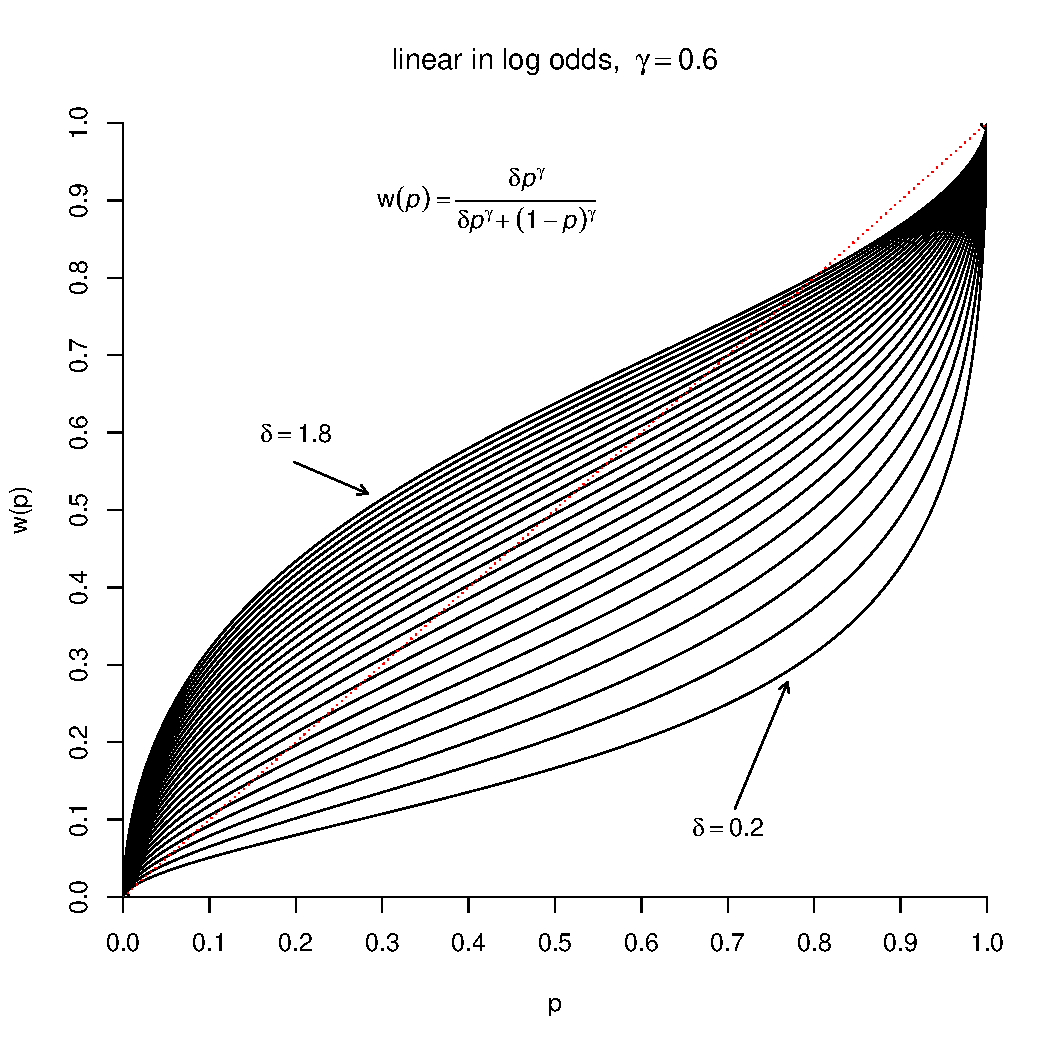
\includegraphics[width=\maxwidth]{figure/unnamed-chunk-22} 

}



\end{knitrout}


Likewise, {\bf pt} can be used to show the effects of varying $\gamma$ on the curvature. Lower values of $\gamma$ increase the curvature.

\begin{knitrout}
\definecolor{shadecolor}{rgb}{0.969, 0.969, 0.969}\color{fgcolor}\begin{kframe}
\begin{alltt}
\hlkwd{plotTwoParProbWFam}\hlstd{(}\hlkwc{my_title}\hlstd{=}\hlkwd{expression}\hlstd{(}\hlkwd{paste}\hlstd{(}\hlstr{"linear in log odds,  "}\hlstd{,}
        \hlstd{delta} \hlopt{==} \hlnum{0.6}\hlstd{)),}
        \hlkwc{my_title_colour}\hlstd{=}\hlstr{"black"}\hlstd{,} \hlkwc{my_title_font_size}\hlstd{=}\hlnum{4}\hlstd{,}
        \hlkwc{my_x_label} \hlstd{=} \hlstr{"p"}\hlstd{,} \hlkwc{my_y_label} \hlstd{=} \hlstr{"w(p)"}\hlstd{,} \hlkwc{pwf}\hlstd{=linear_in_log_odds_pwf,}
        \hlkwc{par}\hlstd{=}\hlkwd{list}\hlstd{(}\hlkwc{a_list}\hlstd{=}\hlkwd{seq}\hlstd{(}\hlkwc{from}\hlstd{=}\hlnum{0.2}\hlstd{,} \hlkwc{to}\hlstd{=}\hlnum{1.8}\hlstd{,} \hlkwc{by}\hlstd{=}\hlnum{0.06}\hlstd{),} \hlkwc{b_list}\hlstd{=}\hlkwd{c}\hlstd{(}\hlnum{0.6}\hlstd{)),}
        \hlkwc{draw_reference_line_flag}\hlstd{=}\hlnum{TRUE}\hlstd{,} \hlkwc{reference_line_colour}\hlstd{=}\hlstr{"red"}\hlstd{,}
        \hlkwc{reference_line_style}\hlstd{=}\hlstr{"dotted"}\hlstd{,}
        \hlkwc{my_labels}\hlstd{=}\hlkwd{c}\hlstd{(}\hlkwd{expression}\hlstd{(}\hlkwd{paste}\hlstd{(gamma} \hlopt{==} \hlnum{0.2}\hlstd{)),}
                \hlkwd{expression}\hlstd{(}\hlkwd{paste}\hlstd{(gamma} \hlopt{==} \hlnum{1.8}\hlstd{)),}
                \hlkwd{expression}\hlstd{(}\hlkwd{paste}\hlstd{(}\hlkwd{w}\hlstd{(}\hlkwd{italic}\hlstd{(p))} \hlopt{==} \hlkwd{frac}\hlstd{(delta} \hlopt{*} \hlkwd{italic}\hlstd{(p)}\hlopt{^}\hlstd{gamma,}
                        \hlstd{delta} \hlopt{*} \hlkwd{italic}\hlstd{(p)}\hlopt{^}\hlstd{gamma} \hlopt{+} \hlstd{(}\hlnum{1}\hlopt{-}\hlkwd{italic}\hlstd{(p))}\hlopt{^}\hlstd{gamma)))),}
        \hlkwc{my_label_positions}\hlstd{=}\hlkwd{list}\hlstd{(}\hlkwd{c}\hlstd{(}\hlnum{0.8}\hlstd{,}\hlnum{0.25}\hlstd{),}\hlkwd{c}\hlstd{(}\hlnum{0.5}\hlstd{,}\hlnum{0.1}\hlstd{),}\hlkwd{c}\hlstd{(}\hlnum{0.42}\hlstd{,} \hlnum{0.9}\hlstd{)),}
        \hlkwc{font_scaling}\hlstd{=}\hlnum{1.0}\hlstd{,} \hlkwc{arrow_positions} \hlstd{=} \hlkwd{list}\hlstd{(}\hlkwd{c}\hlstd{(}\hlnum{0.5}\hlstd{,}\hlnum{0.25}\hlstd{,}\hlnum{0.45}\hlstd{,}\hlnum{0.3}\hlstd{),}
                \hlkwd{c}\hlstd{(}\hlnum{0.78}\hlstd{,}\hlnum{0.36}\hlstd{,}\hlnum{0.8}\hlstd{,}\hlnum{0.47}\hlstd{)))}
\end{alltt}
\end{kframe}

{\centering 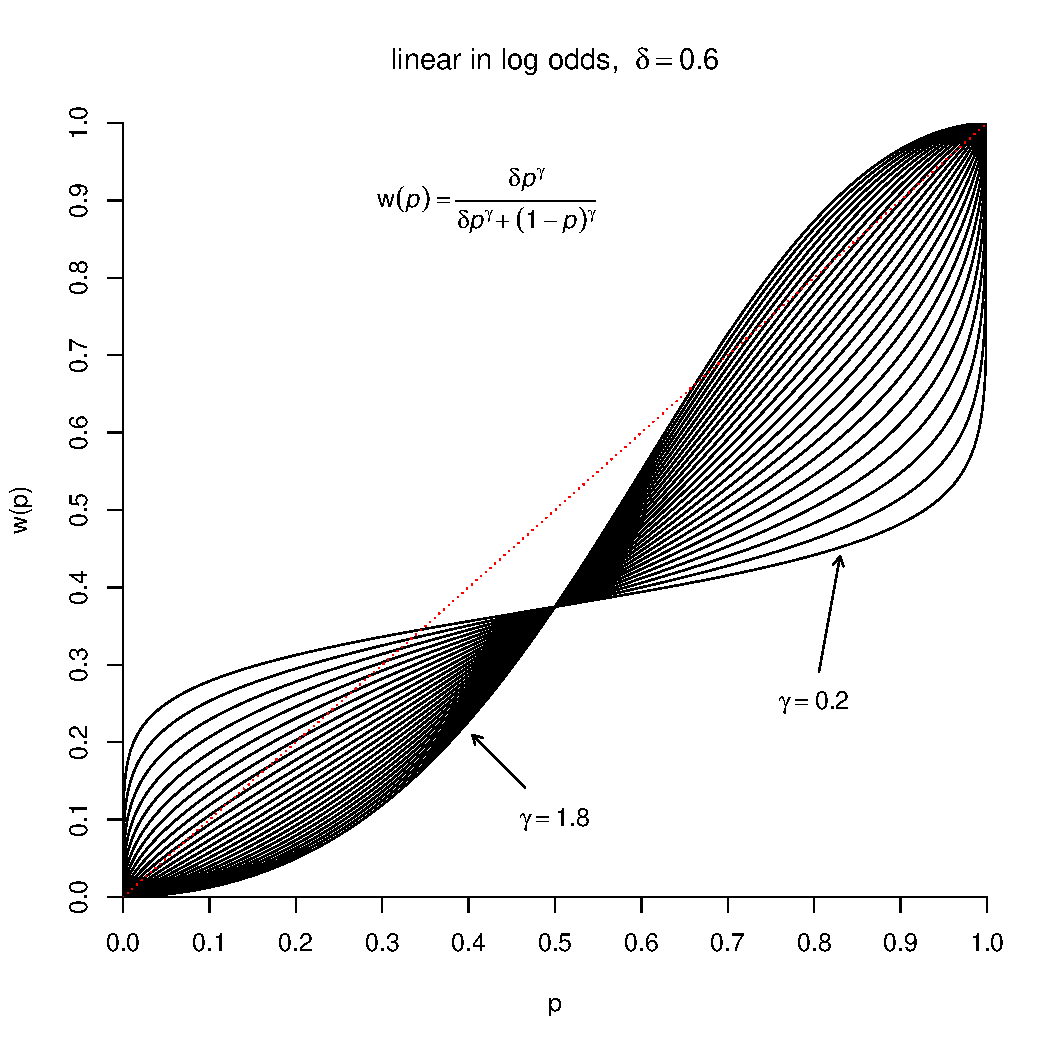
\includegraphics[width=\maxwidth]{figure/unnamed-chunk-23} 

}



\end{knitrout}


Repeating the PT calculations using the \cite{Gonzalez_Wu_1999} probability weighting function gives a similar prediction to before.

\begin{knitrout}
\definecolor{shadecolor}{rgb}{0.969, 0.969, 0.969}\color{fgcolor}\begin{kframe}
\begin{alltt}
\hlstd{tk_1992_utility} \hlkwb{<-} \hlkwd{Utility}\hlstd{(}\hlkwc{fun}\hlstd{=}\hlstr{"power"}\hlstd{,} \hlkwc{par}\hlstd{=}\hlkwd{c}\hlstd{(}\hlkwc{alpha}\hlstd{=}\hlnum{0.88}\hlstd{,} \hlkwc{beta}\hlstd{=}\hlnum{0.88}\hlstd{,} \hlkwc{lambda}\hlstd{=}\hlnum{2.25}\hlstd{))}
\hlstd{linear_in_log_odds_prob_weight} \hlkwb{<-} \hlkwd{ProbWeight}\hlstd{(}\hlkwc{fun}\hlstd{=}\hlstr{"linear_in_log_odds"}\hlstd{,} \hlkwc{par}\hlstd{=}\hlkwd{c}\hlstd{(}\hlkwc{alpha}\hlstd{=}\hlnum{0.61}\hlstd{,} \hlkwc{beta}\hlstd{=}\hlnum{0.724}\hlstd{))}
\hlkwd{comparePT}\hlstd{(my_choices,}
        \hlkwc{prob_weight_for_positive_outcomes}\hlstd{=linear_in_log_odds_prob_weight,}
        \hlkwc{prob_weight_for_negative_outcomes}\hlstd{=linear_in_log_odds_prob_weight,}
        \hlkwc{utility}\hlstd{=tk_1992_utility,} \hlkwc{digits}\hlstd{=}\hlnum{4}\hlstd{)}
\end{alltt}
\begin{verbatim}
##   cid gid   ev    pt    ce                 rp
## 1   1   1 3200 928.1  2357              843.4
## 2   1   2 3000  1148  3000 -0.000000000001819
## 3   2   1  800 350.6 779.4              20.58
## 4   2   2  750 310.2 678.4               71.6
\end{verbatim}
\end{kframe}
\end{knitrout}


Next, SWU predicts the preferences $B > A$ and $C > D$.

\begin{knitrout}
\definecolor{shadecolor}{rgb}{0.969, 0.969, 0.969}\color{fgcolor}\begin{kframe}
\begin{alltt}
\hlstd{my_utility} \hlkwb{<-} \hlkwd{Utility}\hlstd{(}\hlkwc{fun}\hlstd{=}\hlstr{"power"}\hlstd{,} \hlkwc{par}\hlstd{=}\hlkwd{c}\hlstd{(}\hlkwc{alpha}\hlstd{=}\hlnum{0.4}\hlstd{,} \hlkwc{beta}\hlstd{=}\hlnum{0.4}\hlstd{,} \hlkwc{lambda}\hlstd{=}\hlnum{1}\hlstd{))}
\hlstd{my_pwf} \hlkwb{<-} \hlkwd{ProbWeight}\hlstd{(}\hlkwc{fun}\hlstd{=}\hlstr{"linear_in_log_odds"}\hlstd{,} \hlkwc{par}\hlstd{=}\hlkwd{c}\hlstd{(}\hlkwc{alpha}\hlstd{=}\hlnum{0.4}\hlstd{,} \hlkwc{beta}\hlstd{=}\hlnum{0.4}\hlstd{))}
\hlkwd{compareSWU}\hlstd{(my_choices,} \hlkwc{prob_weight}\hlstd{=my_pwf,} \hlkwc{utility}\hlstd{=my_utility,} \hlkwc{digits}\hlstd{=}\hlnum{4}\hlstd{)}
\end{alltt}
\begin{verbatim}
##   cid gid   ev   swu    ce                 rp
## 1   1   1 3200 11.33 431.9               2768
## 2   1   2 3000  24.6  3000 -0.000000000001819
## 3   2   1  800 5.155 60.34              739.7
## 4   2   2  750  5.04 57.04                693
\end{verbatim}
\end{kframe}
\end{knitrout}


SWAU predicts the preferences $B > A$ and $C > D$.

\begin{knitrout}
\definecolor{shadecolor}{rgb}{0.969, 0.969, 0.969}\color{fgcolor}\begin{kframe}
\begin{alltt}
\hlstd{my_utility} \hlkwb{<-} \hlkwd{Utility}\hlstd{(}\hlkwc{fun}\hlstd{=}\hlstr{"power"}\hlstd{,} \hlkwc{par}\hlstd{=}\hlkwd{c}\hlstd{(}\hlkwc{alpha}\hlstd{=}\hlnum{0.4}\hlstd{,} \hlkwc{beta}\hlstd{=}\hlnum{0.4}\hlstd{,} \hlkwc{lambda}\hlstd{=}\hlnum{1}\hlstd{))}
\hlstd{my_pwf} \hlkwb{<-} \hlkwd{ProbWeight}\hlstd{(}\hlkwc{fun}\hlstd{=}\hlstr{"linear_in_log_odds"}\hlstd{,} \hlkwc{par}\hlstd{=}\hlkwd{c}\hlstd{(}\hlkwc{alpha}\hlstd{=}\hlnum{0.4}\hlstd{,} \hlkwc{beta}\hlstd{=}\hlnum{0.4}\hlstd{))}
\hlkwd{compareSWAU}\hlstd{(my_choices,} \hlkwc{prob_weight}\hlstd{=my_pwf,} \hlkwc{utility}\hlstd{=my_utility,} \hlkwc{digits}\hlstd{=}\hlnum{4}\hlstd{)}
\end{alltt}
\begin{verbatim}
##   cid gid   ev  swau    ce                 rp
## 1   1   1 3200 18.96  1566               1634
## 2   1   2 3000  24.6  3000 -0.000000000001819
## 3   2   1  800  8.63 218.8              581.2
## 4   2   2  750 8.573 215.2              534.8
\end{verbatim}
\end{kframe}
\end{knitrout}


RAM predicts the preferences $B > A$ and $C > D$.

\begin{knitrout}
\definecolor{shadecolor}{rgb}{0.969, 0.969, 0.969}\color{fgcolor}\begin{kframe}
\begin{alltt}
\hlstd{branch_weight_list} \hlkwb{<-} \hlkwd{list}\hlstd{(}\hlkwd{c}\hlstd{(}\hlnum{1}\hlstd{),} \hlkwd{c}\hlstd{(}\hlnum{0.3738}\hlstd{,} \hlnum{0.6262}\hlstd{))}
\hlstd{my_utility} \hlkwb{<-} \hlkwd{Utility}\hlstd{(}\hlkwc{fun}\hlstd{=}\hlstr{"linear"}\hlstd{,} \hlkwc{par}\hlstd{=}\hlkwd{c}\hlstd{(}\hlkwc{lambda}\hlstd{=}\hlnum{1}\hlstd{))}
\hlstd{power_prob_weight} \hlkwb{<-} \hlkwd{ProbWeight}\hlstd{(}\hlkwc{fun}\hlstd{=}\hlstr{"power"}\hlstd{,} \hlkwc{par}\hlstd{=}\hlkwd{c}\hlstd{(}\hlkwc{alpha}\hlstd{=}\hlnum{0.7}\hlstd{,} \hlkwc{beta}\hlstd{=}\hlnum{1}\hlstd{))}
\hlkwd{compareRAM}\hlstd{(my_choices,} \hlkwc{branch_weight_list}\hlstd{=branch_weight_list,}
        \hlkwc{prob_weight}\hlstd{=power_prob_weight,} \hlkwc{utility}\hlstd{=my_utility,} \hlkwc{digits}\hlstd{=}\hlnum{4}\hlstd{)}
\end{alltt}
\begin{verbatim}
##   cid gid   ev  ramu    ce    rp
## 1   1   1 3200  2447  2447 753.2
## 2   1   2 3000  3000  3000     0
## 3   2   1  800 737.9 737.9 62.12
## 4   2   2  750 650.1 650.1 99.89
\end{verbatim}
\end{kframe}
\end{knitrout}


GDU predicts the preferences $B > A$ and $C > D$.

\begin{knitrout}
\definecolor{shadecolor}{rgb}{0.969, 0.969, 0.969}\color{fgcolor}\begin{kframe}
\begin{alltt}
\hlstd{my_pwf} \hlkwb{<-} \hlkwd{ProbWeight}\hlstd{(}\hlkwc{fun}\hlstd{=}\hlstr{"compound_invariance"}\hlstd{,} \hlkwc{par}\hlstd{=}\hlkwd{c}\hlstd{(}\hlkwc{alpha}\hlstd{=}\hlnum{0.542}\hlstd{,} \hlkwc{beta}\hlstd{=}\hlnum{1.382}\hlstd{))}
\hlstd{my_utility} \hlkwb{<-} \hlkwd{Utility}\hlstd{(}\hlkwc{fun}\hlstd{=}\hlstr{"power"}\hlstd{,} \hlkwc{par}\hlstd{=}\hlkwd{c}\hlstd{(}\hlkwc{alpha}\hlstd{=}\hlnum{1}\hlstd{,} \hlkwc{beta}\hlstd{=}\hlnum{1}\hlstd{,} \hlkwc{lambda}\hlstd{=}\hlnum{1}\hlstd{))}
\hlkwd{compareGDU}\hlstd{(my_choices,} \hlkwc{prob_weight}\hlstd{=my_pwf,} \hlkwc{utility}\hlstd{=my_utility,} \hlkwc{digits}\hlstd{=}\hlnum{4}\hlstd{)}
\end{alltt}
\begin{verbatim}
##   cid gid   ev   gdu    ce    rp
## 1   1   1 3200  2167  2167  1033
## 2   1   2 3000  3000  3000     0
## 3   2   1  800 668.7 668.7 131.3
## 4   2   2  750 576.3 576.3 173.7
\end{verbatim}
\end{kframe}
\end{knitrout}


PRT predicts the preferences $B > A$ and $C > D$.

\begin{knitrout}
\definecolor{shadecolor}{rgb}{0.969, 0.969, 0.969}\color{fgcolor}\begin{kframe}
\begin{alltt}
\hlstd{my_utility} \hlkwb{<-} \hlkwd{Utility}\hlstd{(}\hlkwc{fun}\hlstd{=}\hlstr{"power"}\hlstd{,} \hlkwc{par}\hlstd{=}\hlkwd{c}\hlstd{(}\hlkwc{alpha}\hlstd{=}\hlnum{0.631}\hlstd{,} \hlkwc{beta}\hlstd{=}\hlnum{0.631}\hlstd{,} \hlkwc{lambda}\hlstd{=}\hlnum{1}\hlstd{))}
\hlkwd{comparePRT}\hlstd{(my_choices,} \hlkwc{utility}\hlstd{=my_utility,} \hlkwc{gamma}\hlstd{=}\hlnum{0.676}\hlstd{,} \hlkwc{digits}\hlstd{=}\hlnum{4}\hlstd{)}
\end{alltt}
\begin{verbatim}
##   cid gid   ev  prtu    ce                  rp
## 1   1   1 3200 131.7  2287               912.7
## 2   1   2 3000 156.3  3000 -0.0000000000004547
## 3   2   1  800 55.71 584.7               215.3
## 4   2   2  750 51.75 520.2               229.8
\end{verbatim}
\end{kframe}
\end{knitrout}


TAX predicts the preferences $B > A$ and $C > D$.

\begin{knitrout}
\definecolor{shadecolor}{rgb}{0.969, 0.969, 0.969}\color{fgcolor}\begin{kframe}
\begin{alltt}
\hlstd{my_utility} \hlkwb{<-} \hlkwd{Utility}\hlstd{(}\hlkwc{fun}\hlstd{=}\hlstr{"linear"}\hlstd{,} \hlkwc{par}\hlstd{=}\hlkwd{c}\hlstd{(}\hlkwc{lambda}\hlstd{=}\hlnum{1}\hlstd{))}
\hlstd{power_prob_weight} \hlkwb{<-} \hlkwd{ProbWeight}\hlstd{(}\hlkwc{fun}\hlstd{=}\hlstr{"power"}\hlstd{,} \hlkwc{par}\hlstd{=}\hlkwd{c}\hlstd{(}\hlkwc{alpha}\hlstd{=}\hlnum{0.7}\hlstd{,} \hlkwc{beta}\hlstd{=}\hlnum{1}\hlstd{))}
\hlkwd{compareTAX}\hlstd{(my_choices,} \hlkwc{prob_weight}\hlstd{=power_prob_weight,} \hlkwc{utility}\hlstd{=my_utility,} \hlkwc{delta}\hlstd{=}\hlopt{-}\hlnum{1}\hlstd{,} \hlkwc{digits}\hlstd{=}\hlnum{4}\hlstd{)}
\end{alltt}
\begin{verbatim}
##   cid gid   ev   tax    ce    rp
## 1   1   1 3200  1934  1934  1266
## 2   1   2 3000  3000  3000     0
## 3   2   1  800 732.8 732.8  67.2
## 4   2   2  750 633.4 633.4 116.6
\end{verbatim}
\end{kframe}
\end{knitrout}


Note that this TAX example uses a linear probability weighting function. TAX explains the Allais paradoxes through the increased branch weighting given to the lowest branches of a choice.
Given there are three objective consequences $\{0, 3000, 4000\}$, we can show the gambles in the
probability simplex. The iso-expected value lines are shown in black, the expected utility indifference lines in purple and the prospect theory indifference curves in red.

\begin{knitrout}
\definecolor{shadecolor}{rgb}{0.969, 0.969, 0.969}\color{fgcolor}\begin{kframe}
\begin{alltt}
\hlstd{my_utility} \hlkwb{<-} \hlkwd{Utility}\hlstd{(}\hlkwc{fun}\hlstd{=}\hlstr{"power"}\hlstd{,} \hlkwc{par}\hlstd{=}\hlkwd{c}\hlstd{(}\hlkwc{alpha}\hlstd{=}\hlnum{0.88}\hlstd{,} \hlkwc{beta}\hlstd{=}\hlnum{0.88}\hlstd{,} \hlkwc{lambda}\hlstd{=}\hlnum{1}\hlstd{))}

\hlkwd{drawSimplex}\hlstd{(}\hlkwc{x1}\hlstd{=}\hlnum{0}\hlstd{,} \hlkwc{x2}\hlstd{=}\hlnum{3000}\hlstd{,} \hlkwc{x3}\hlstd{=}\hlnum{4000}\hlstd{,}
        \hlkwc{line_dot_density}\hlstd{=}\hlnum{1000}\hlstd{,}
        \hlkwc{draw_ev_flag}\hlstd{=}\hlnum{TRUE}\hlstd{,} \hlkwc{ev_colour}\hlstd{=}\hlstr{"black"}\hlstd{,}
        \hlkwc{draw_pt_flag}\hlstd{=}\hlnum{TRUE}\hlstd{,} \hlkwc{alpha}\hlstd{=}\hlnum{0.61}\hlstd{,} \hlkwc{beta}\hlstd{=}\hlnum{0.724}\hlstd{,} \hlkwc{pt_colour}\hlstd{=}\hlstr{"red"}\hlstd{,}
        \hlkwc{draw_utility_flag}\hlstd{=}\hlnum{TRUE}\hlstd{,} \hlkwc{utility}\hlstd{=my_utility,} \hlkwc{eu_colour}\hlstd{=}\hlstr{"purple"}\hlstd{,}
        \hlkwc{start_points}\hlstd{=}\hlkwd{list}\hlstd{(}\hlkwd{c}\hlstd{(}\hlnum{0.1}\hlstd{,}\hlnum{0.9}\hlstd{),}\hlkwd{c}\hlstd{(}\hlnum{0.2}\hlstd{,}\hlnum{0.8}\hlstd{),}\hlkwd{c}\hlstd{(}\hlnum{0.3}\hlstd{,}\hlnum{0.7}\hlstd{),}\hlkwd{c}\hlstd{(}\hlnum{0.4}\hlstd{,}\hlnum{0.6}\hlstd{),}
                \hlkwd{c}\hlstd{(}\hlnum{0.5}\hlstd{,}\hlnum{0.5}\hlstd{),}\hlkwd{c}\hlstd{(}\hlnum{0.6}\hlstd{,}\hlnum{0.4}\hlstd{),}\hlkwd{c}\hlstd{(}\hlnum{0.7}\hlstd{,}\hlnum{0.3}\hlstd{),}\hlkwd{c}\hlstd{(}\hlnum{0.8}\hlstd{,}\hlnum{0.2}\hlstd{),}\hlkwd{c}\hlstd{(}\hlnum{0.9}\hlstd{,}\hlnum{0.1}\hlstd{)),}
        \hlkwc{labels}\hlstd{=}\hlkwd{c}\hlstd{(}\hlstr{"A"}\hlstd{,}\hlstr{"B"}\hlstd{,}\hlstr{"C"}\hlstd{,}\hlstr{"D"}\hlstd{,}\hlstr{"increasing preference"}\hlstd{),}
        \hlkwc{label_positions}\hlstd{=}\hlkwd{list}\hlstd{(}\hlkwd{c}\hlstd{(}\hlnum{0.03}\hlstd{,}\hlnum{0.04}\hlstd{),}\hlkwd{c}\hlstd{(}\hlnum{0.21}\hlstd{,}\hlnum{0.75}\hlstd{),}
                \hlkwd{c}\hlstd{(}\hlnum{0.79}\hlstd{,}\hlnum{0.04}\hlstd{),}\hlkwd{c}\hlstd{(}\hlnum{0.85}\hlstd{,}\hlnum{0.18}\hlstd{),}\hlkwd{c}\hlstd{(}\hlnum{0.7}\hlstd{,}\hlnum{0.7}\hlstd{)),}
        \hlkwc{label_colours}\hlstd{=}\hlkwd{c}\hlstd{(}\hlstr{"orange"}\hlstd{,}\hlstr{"purple"}\hlstd{,}\hlstr{"orange"}\hlstd{,}\hlstr{"purple"}\hlstd{,}\hlstr{"red"}\hlstd{),}
        \hlkwc{label_font_sizes}\hlstd{=}\hlkwd{c}\hlstd{(}\hlnum{12}\hlstd{,}\hlnum{12}\hlstd{,}\hlnum{12}\hlstd{,}\hlnum{12}\hlstd{,}\hlnum{16}\hlstd{),}
        \hlkwc{label_font_faces}\hlstd{=}\hlkwd{c}\hlstd{(}\hlstr{"plain"}\hlstd{,}\hlstr{"plain"}\hlstd{,}\hlstr{"plain"}\hlstd{,}\hlstr{"plain"}\hlstd{,}\hlstr{"bold"}\hlstd{),}
        \hlkwc{label_rotations}\hlstd{=}\hlkwd{c}\hlstd{(}\hlnum{0}\hlstd{,}\hlnum{0}\hlstd{,}\hlnum{0}\hlstd{,}\hlnum{0}\hlstd{,}\hlopt{-}\hlnum{45}\hlstd{),}
        \hlkwc{circle_radii}\hlstd{=}\hlkwd{c}\hlstd{(}\hlnum{0.01}\hlstd{,}\hlnum{0.01}\hlstd{,}\hlnum{0.01}\hlstd{,}\hlnum{0.01}\hlstd{),}
        \hlkwc{circle_outline_colours}\hlstd{=}\hlkwd{c}\hlstd{(}\hlstr{"black"}\hlstd{,}\hlstr{"black"}\hlstd{,}\hlstr{"black"}\hlstd{,}\hlstr{"black"}\hlstd{),}
        \hlkwc{circle_fill_colours}\hlstd{=}\hlkwd{c}\hlstd{(}\hlstr{"orange"}\hlstd{,}\hlstr{"purple"}\hlstd{,}\hlstr{"orange"}\hlstd{,}\hlstr{"purple"}\hlstd{),}
        \hlkwc{circle_positions}\hlstd{=}\hlkwd{list}\hlstd{(}\hlkwd{c}\hlstd{(}\hlnum{0}\hlstd{,}\hlnum{0}\hlstd{),}\hlkwd{c}\hlstd{(}\hlnum{0.2}\hlstd{,}\hlnum{0.8}\hlstd{),}\hlkwd{c}\hlstd{(}\hlnum{0.75}\hlstd{,}\hlnum{0}\hlstd{),}\hlkwd{c}\hlstd{(}\hlnum{0.8}\hlstd{,}\hlnum{0.2}\hlstd{)),}
        \hlkwc{lines}\hlstd{=}\hlkwd{list}\hlstd{(}\hlkwd{c}\hlstd{(}\hlnum{0}\hlstd{,}\hlnum{0}\hlstd{,}\hlnum{0.2}\hlstd{,}\hlnum{0.8}\hlstd{),}\hlkwd{c}\hlstd{(}\hlnum{0.2}\hlstd{,}\hlnum{0.8}\hlstd{,}\hlnum{0.8}\hlstd{,}\hlnum{0.2}\hlstd{),}
                \hlkwd{c}\hlstd{(}\hlnum{0.8}\hlstd{,}\hlnum{0.2}\hlstd{,}\hlnum{0.75}\hlstd{,}\hlnum{0}\hlstd{),}\hlkwd{c}\hlstd{(}\hlnum{0.75}\hlstd{,}\hlnum{0}\hlstd{,}\hlnum{0}\hlstd{,}\hlnum{0}\hlstd{)),}
        \hlkwc{line_widths}\hlstd{=}\hlkwd{c}\hlstd{(}\hlnum{1}\hlstd{,} \hlnum{1}\hlstd{,} \hlnum{1}\hlstd{,} \hlnum{1}\hlstd{),}
        \hlkwc{line_styles}\hlstd{=}\hlkwd{c}\hlstd{(}\hlstr{"dashed"}\hlstd{,} \hlstr{"dashed"}\hlstd{,} \hlstr{"dashed"}\hlstd{,} \hlstr{"dashed"}\hlstd{),}
        \hlkwc{line_colours}\hlstd{=}\hlkwd{c}\hlstd{(}\hlstr{"blue"}\hlstd{,}\hlstr{"blue"}\hlstd{,}\hlstr{"blue"}\hlstd{,}\hlstr{"blue"}\hlstd{),}
        \hlkwc{arrows}\hlstd{=}\hlkwd{list}\hlstd{(}\hlkwd{c}\hlstd{(}\hlnum{0.8}\hlstd{,}\hlnum{0.5}\hlstd{,}\hlnum{0.5}\hlstd{,}\hlnum{0.8}\hlstd{)),}
        \hlkwc{arrow_widths}\hlstd{=}\hlkwd{c}\hlstd{(}\hlnum{2}\hlstd{),} \hlkwc{arrow_styles}\hlstd{=}\hlkwd{c}\hlstd{(}\hlstr{"solid"}\hlstd{),} \hlkwc{arrow_colours}\hlstd{=}\hlkwd{c}\hlstd{(}\hlstr{"red"}\hlstd{))}
\end{alltt}
\end{kframe}

{\centering 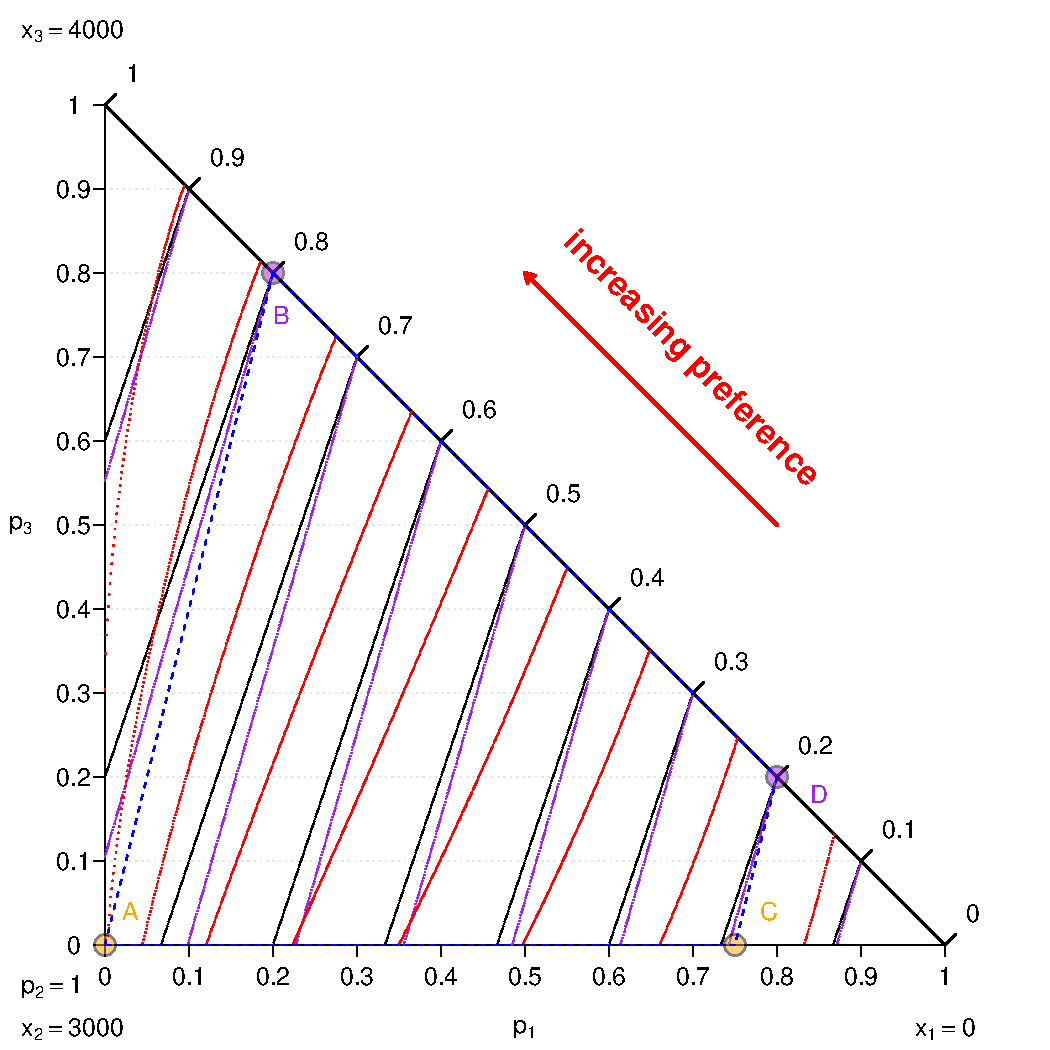
\includegraphics[width=0.8\linewidth]{figure/unnamed-chunk-31} 

}



\end{knitrout}


The introduction of a reference point allowed PT to generated novel predictions such as the four-fold pattern of risk attitudes and loss aversion. These successes will be described in the following sections.

\section{Four-fold pattern of risk attitudes}

One of the most distinctive predictions of prospect theory has been the four-fold pattern of risk attitudes within
individual decision makers. Although EU could predict both risk aversion and risk seeking using different utility curves, it could not do this simultaneously in the same decision maker.
The combination of reference points, curvature of the probability weighting function and kinked utility function allows PT to model this pattern.
A key concept in PT is outcomes are regarded as losses or gains relative to a reference point defined via a framing event.
The reference point is generally taken to be the ``status quo''.
Put very roughly, people don't mind winning, but are averse to losing. To capture this effect, losses are weighted more than gains. Small probability outcomes are overestimated relative to the actual probability of the outcome happening.
Middle and high probability outcomes are underweighted relative to the actual probabilities of these outcomes.
Negative outcomes are given more weight (loss aversion). The weight of rare events is increased.
The predictions are given in Table \ref{four_fold_table}.

\begin{table}[h]
\caption{Four-fold pattern of risk attitudes.}
\centering
\begin{tabular}{ r|c|c| }
\multicolumn{1}{r}{}
 &  \multicolumn{1}{c}{medium to high probability event}
 & \multicolumn{1}{c}{low probability event} \\
\cline{2-3}
loss & risk seeking & risk averse \\
\cline{2-3}
gain & risk averse & risk seeking \\
\cline{2-3}
\end{tabular}
\label{four_fold_table}
\end{table}

Consider problems 11, 12. 14 and 14' from \citet[][p. 273, 281]{Kahneman_Tversky_1979} which illustrate the four-fold pattern.

\begin{knitrout}
\definecolor{shadecolor}{rgb}{0.969, 0.969, 0.969}\color{fgcolor}\begin{kframe}
\begin{alltt}
\hlstd{choice_ids} \hlkwb{<-} \hlkwd{c}\hlstd{(}\hlnum{1}\hlstd{,} \hlnum{1}\hlstd{,} \hlnum{1}\hlstd{,} \hlnum{2}\hlstd{,} \hlnum{2}\hlstd{,} \hlnum{2}\hlstd{,} \hlnum{3}\hlstd{,} \hlnum{3}\hlstd{,} \hlnum{3}\hlstd{,} \hlnum{4}\hlstd{,} \hlnum{4}\hlstd{,} \hlnum{4}\hlstd{)}
\hlstd{gamble_ids} \hlkwb{<-} \hlkwd{c}\hlstd{(}\hlnum{1}\hlstd{,} \hlnum{1}\hlstd{,} \hlnum{2}\hlstd{,} \hlnum{1}\hlstd{,} \hlnum{1}\hlstd{,} \hlnum{2}\hlstd{,} \hlnum{1}\hlstd{,} \hlnum{1}\hlstd{,} \hlnum{2}\hlstd{,} \hlnum{1}\hlstd{,} \hlnum{1}\hlstd{,} \hlnum{2}\hlstd{)}
\hlstd{outcome_ids} \hlkwb{<-} \hlkwd{c}\hlstd{(}\hlnum{1}\hlstd{,} \hlnum{2}\hlstd{,} \hlnum{1}\hlstd{,} \hlnum{1}\hlstd{,} \hlnum{2}\hlstd{,} \hlnum{1}\hlstd{,} \hlnum{1}\hlstd{,} \hlnum{2}\hlstd{,} \hlnum{1}\hlstd{,} \hlnum{1}\hlstd{,} \hlnum{2}\hlstd{,} \hlnum{1}\hlstd{)}
\hlstd{objective_consequences} \hlkwb{<-} \hlkwd{c}\hlstd{(}\hlnum{1000}\hlstd{,} \hlnum{0}\hlstd{,} \hlnum{500}\hlstd{,} \hlopt{-}\hlnum{0}\hlstd{,} \hlopt{-}\hlnum{1000}\hlstd{,} \hlopt{-}\hlnum{500}\hlstd{,}
        \hlnum{5000}\hlstd{,} \hlnum{0}\hlstd{,} \hlnum{5}\hlstd{,} \hlopt{-}\hlnum{5000}\hlstd{,} \hlopt{-}\hlnum{0}\hlstd{,} \hlopt{-}\hlnum{5}\hlstd{)}
\hlstd{probability_strings} \hlkwb{<-} \hlkwd{c}\hlstd{(}\hlstr{"1/2"}\hlstd{,} \hlstr{"1/2"}\hlstd{,} \hlstr{"1"}\hlstd{,} \hlstr{"1/2"}\hlstd{,} \hlstr{"1/2"}\hlstd{,}
        \hlstr{"1"}\hlstd{,} \hlstr{"0.001"}\hlstd{,} \hlstr{"0.999"}\hlstd{,} \hlstr{"1"}\hlstd{,} \hlstr{"0.001"}\hlstd{,} \hlstr{"0.999"}\hlstd{,} \hlstr{"1"}\hlstd{)}
\hlstd{my_choices} \hlkwb{<-} \hlkwd{Choices}\hlstd{(}\hlkwc{choice_ids}\hlstd{=choice_ids,}
        \hlkwc{gamble_ids}\hlstd{=gamble_ids,}
        \hlkwc{outcome_ids}\hlstd{=outcome_ids,}
        \hlkwc{objective_consequences}\hlstd{=objective_consequences,}
        \hlkwc{probability_strings}\hlstd{=probability_strings)}
\hlstd{my_choices}
\end{alltt}
\begin{verbatim}
##    cid gid oid    pr    oc
## 1    1   1   1   1/2  1000
## 2    1   1   2   1/2     0
## 3    1   2   1     1   500
## 4    2   1   1   1/2     0
## 5    2   1   2   1/2 -1000
## 6    2   2   1     1  -500
## 7    3   1   1 0.001  5000
## 8    3   1   2 0.999     0
## 9    3   2   1     1     5
## 10   4   1   1 0.001 -5000
## 11   4   1   2 0.999     0
## 12   4   2   1     1    -5
\end{verbatim}
\begin{alltt}
\hlkwd{drawChoices}\hlstd{(my_choices,}
        \hlkwc{decision_square_x}\hlstd{=}\hlnum{0.2}\hlstd{,} \hlkwc{decision_square_edge_length}\hlstd{=}\hlnum{0.03}\hlstd{,}
        \hlkwc{circle_radius}\hlstd{=}\hlnum{0.02}\hlstd{,} \hlkwc{y_split_gap}\hlstd{=}\hlnum{0.07}\hlstd{,} \hlkwc{x_split_offset}\hlstd{=}\hlnum{0.03}\hlstd{,}
        \hlkwc{probability_text_digits}\hlstd{=}\hlnum{4}\hlstd{,} \hlkwc{y_probability_text_offset}\hlstd{=}\hlnum{0.015}\hlstd{,}
        \hlkwc{y_value_text_offset}\hlstd{=}\hlnum{0.005}\hlstd{,} \hlkwc{x_value_text_offset}\hlstd{=}\hlnum{0.025}\hlstd{,}
        \hlkwc{probability_text_font_colour}\hlstd{=}\hlstr{"red"}\hlstd{,} \hlkwc{probability_text_font_size}\hlstd{=}\hlnum{10}\hlstd{,}
        \hlkwc{objective_consequence_text_font_colour}\hlstd{=}\hlstr{"blue"}\hlstd{,}
        \hlkwc{objective_consequence_text_font_size}\hlstd{=}\hlnum{10}\hlstd{,}
        \hlkwc{label}\hlstd{=}\hlkwd{c}\hlstd{(}\hlstr{"A"}\hlstd{,}\hlstr{"B"}\hlstd{,}\hlstr{"C"}\hlstd{,}\hlstr{"D"}\hlstd{,}\hlstr{"E"}\hlstd{,}\hlstr{"F"}\hlstd{,}\hlstr{"G"}\hlstd{,}\hlstr{"H"}\hlstd{),}
        \hlkwc{label_font_colour}\hlstd{=}\hlkwd{c}\hlstd{(}\hlstr{"orange"}\hlstd{,}\hlstr{"magenta"}\hlstd{,}\hlstr{"green"}\hlstd{,}\hlstr{"blue"}\hlstd{,}
                \hlstr{"purple"}\hlstd{,}\hlstr{"pink"}\hlstd{,}\hlstr{"grey"}\hlstd{,}\hlstr{"violet"}\hlstd{),}
        \hlkwc{label_font_size}\hlstd{=}\hlkwd{c}\hlstd{(}\hlnum{11}\hlstd{,}\hlnum{11}\hlstd{,}\hlnum{11}\hlstd{,}\hlnum{11}\hlstd{,}\hlnum{11}\hlstd{,}\hlnum{11}\hlstd{,}\hlnum{11}\hlstd{,}\hlnum{11}\hlstd{),}
        \hlkwc{label_positions}\hlstd{=}\hlkwd{list}\hlstd{(}\hlkwd{c}\hlstd{(}\hlnum{0.26}\hlstd{,}\hlnum{0.94}\hlstd{),}\hlkwd{c}\hlstd{(}\hlnum{0.26}\hlstd{,}\hlnum{0.78}\hlstd{),}\hlkwd{c}\hlstd{(}\hlnum{0.26}\hlstd{,}\hlnum{0.69}\hlstd{),}
                \hlkwd{c}\hlstd{(}\hlnum{0.26}\hlstd{,}\hlnum{0.53}\hlstd{),}\hlkwd{c}\hlstd{(}\hlnum{0.26}\hlstd{,}\hlnum{0.44}\hlstd{),}\hlkwd{c}\hlstd{(}\hlnum{0.26}\hlstd{,}\hlnum{0.28}\hlstd{),}\hlkwd{c}\hlstd{(}\hlnum{0.26}\hlstd{,}\hlnum{0.2}\hlstd{),}
                \hlkwd{c}\hlstd{(}\hlnum{0.26}\hlstd{,}\hlnum{0.03}\hlstd{)))}
\end{alltt}
\end{kframe}

{\centering 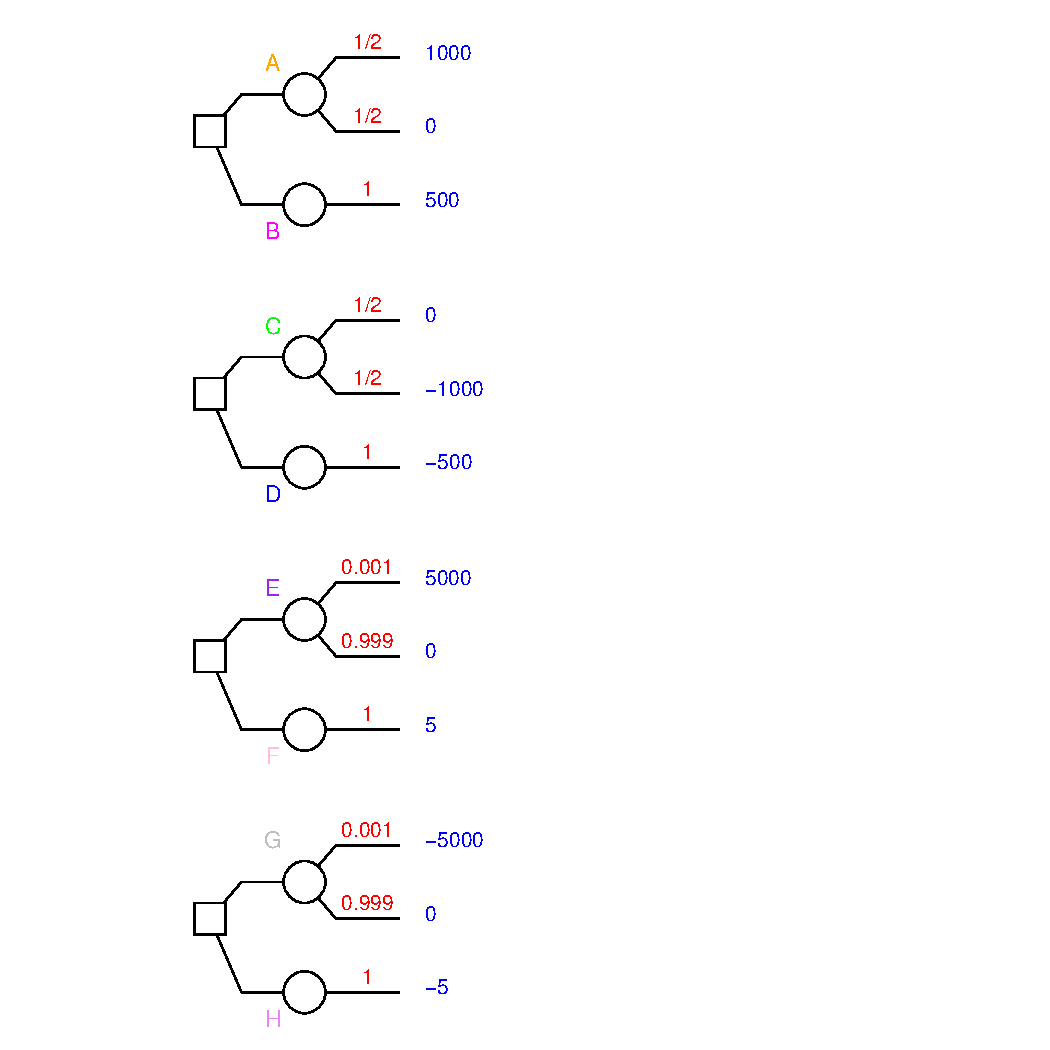
\includegraphics[width=0.8\linewidth]{figure/unnamed-chunk-32} 

}



\end{knitrout}


The PT predictions can be calculated as follows.

\begin{knitrout}
\definecolor{shadecolor}{rgb}{0.969, 0.969, 0.969}\color{fgcolor}\begin{kframe}
\begin{alltt}
\hlstd{tk_1992_utility} \hlkwb{<-} \hlkwd{Utility}\hlstd{(}\hlkwc{fun}\hlstd{=}\hlstr{"power"}\hlstd{,} \hlkwc{par}\hlstd{=}\hlkwd{c}\hlstd{(}\hlkwc{alpha}\hlstd{=}\hlnum{0.88}\hlstd{,} \hlkwc{beta}\hlstd{=}\hlnum{0.88}\hlstd{,} \hlkwc{lambda}\hlstd{=}\hlnum{2.25}\hlstd{))}
\hlstd{linear_in_log_odds_prob_weight} \hlkwb{<-} \hlkwd{ProbWeight}\hlstd{(}\hlkwc{fun}\hlstd{=}\hlstr{"linear_in_log_odds"}\hlstd{,} \hlkwc{par}\hlstd{=}\hlkwd{c}\hlstd{(}\hlkwc{alpha}\hlstd{=}\hlnum{0.61}\hlstd{,} \hlkwc{beta}\hlstd{=}\hlnum{0.724}\hlstd{))}
\hlkwd{comparePT}\hlstd{(my_choices,}
        \hlkwc{prob_weight_for_positive_outcomes}\hlstd{=linear_in_log_odds_prob_weight,}
        \hlkwc{prob_weight_for_negative_outcomes}\hlstd{=linear_in_log_odds_prob_weight,}
        \hlkwc{utility}\hlstd{=tk_1992_utility,} \hlkwc{digits}\hlstd{=}\hlnum{4}\hlstd{)}
\end{alltt}
\begin{verbatim}
##   cid gid   ev     pt     ce                     rp
## 1   1   1  500  183.3  373.1                  126.9
## 2   1   2  500  237.2    500    -0.0000000000002842
## 3   2   1 -500 -412.5 -373.1                 -126.9
## 4   2   2 -500 -533.7   -500     0.0000000000002842
## 5   3   1    5  19.08  28.52                 -23.52
## 6   3   2    5  4.122      5 -0.0000000000000008882
## 7   4   1   -5 -42.92 -28.52                  23.52
## 8   4   2   -5 -9.274     -5  0.0000000000000008882
\end{verbatim}
\end{kframe}
\end{knitrout}


\cite{Kahneman_Tversky_1979} found empirical support for the PT predictions. These results are illustrated in
Table \ref{reflection_effect_table}.

\begin{table}[h]
\caption{Reflection effect patterns \cite[from][]{Kahneman_Tversky_1979}.}
\centering
\begin{tabular}{ l l l l l l }
\hline
Problem 11. (p. 273) \\
Risk averse for potential large gains under medium to high probability & (B $>$ A) & $84\%$ & $N=70$ \\
Problem 12. (p. 273) \\
Risk seeking to avoid potential large losses & (C $>$ D) & $69\%$ & $N=68$ \\
Problem 14. (p. 281) \\
Risk seeking for highly unlikely large gains (Gambling) & (E $>$ F) & $72\%$ & $N=72$ \\
Problem 14'. (p. 281) \\
Risk averse for highly unlikely large losses (Insurance) & (H $>$ G) & $83\%$ & $N=72$ \\
\hline
\end{tabular}
\label{reflection_effect_table}
\end{table}

The first two choices are exactly the same choices but are framed differently.
A sample of $70$ subjects were given $1000$ in choice 1 and $68$ different subjects were given $2000$ in choice 2. They were then asked to make two choices. In choice 1 $84\%$ preferred $B > A$. In choice 2 $69\%$ preferred $C > D$. However, the end states are the same in both choices: $1500$ for certain for options $B$ and $D$ and an equal chance gamble to gain $1000$ or $2000$ for options $A$ and $C$. In the first choice (a gains frame), people exhibited risk aversion while in the second choice (a loss frame) they exhibited risk seeking. These patterns have been empirically supported by other researchers, however the patterns may be sensitive to different elicitation procedures. \citet[][]{Harbaugh_Krause_Vesterlund_2010} found more complex choice elicitation procedures led to greater support for the four-fold pattern compared to simpler procedures,
and suggest increased cognitive load may be responsible for the four-fold pattern. Prospect theory can
also predict the (M4) \cite{Markowitz_1952} four-fold pattern of risk preferences for outcome magnitudes  using decreasingly elastic utility functions \cite[][]{Scholten_Read_2014} (see Table \ref{markowitz_four_fold_table}).

\begin{table}[h]
\caption{(M4) Markowitz four-fold pattern for outcome magnitudes.}
\centering
\begin{tabular}{ r|c|c| }
\multicolumn{1}{r}{}
 &  \multicolumn{1}{c}{large outcome}
 & \multicolumn{1}{c}{small outcome} \\
\cline{2-3}
loss & risk seeking & risk averse \\
\cline{2-3}
gain & risk averse & risk seeking \\
\cline{2-3}
\end{tabular}
\label{markowitz_four_fold_table}
\end{table}

To illustrate, consider the following choices from \cite{Hershey_Schoemaker_1980}.

\begin{knitrout}
\definecolor{shadecolor}{rgb}{0.969, 0.969, 0.969}\color{fgcolor}\begin{kframe}
\begin{alltt}
\hlstd{choice_ids} \hlkwb{<-} \hlkwd{c}\hlstd{(}\hlnum{1}\hlstd{,} \hlnum{1}\hlstd{,} \hlnum{1}\hlstd{,} \hlnum{2}\hlstd{,} \hlnum{2}\hlstd{,} \hlnum{2}\hlstd{,} \hlnum{3}\hlstd{,} \hlnum{3}\hlstd{,} \hlnum{3}\hlstd{,} \hlnum{4}\hlstd{,} \hlnum{4}\hlstd{,} \hlnum{4}\hlstd{)}
\hlstd{gamble_ids} \hlkwb{<-} \hlkwd{c}\hlstd{(}\hlnum{1}\hlstd{,} \hlnum{2}\hlstd{,} \hlnum{2}\hlstd{,} \hlnum{1}\hlstd{,} \hlnum{2}\hlstd{,} \hlnum{2}\hlstd{,} \hlnum{1}\hlstd{,} \hlnum{2}\hlstd{,} \hlnum{2}\hlstd{,} \hlnum{1}\hlstd{,} \hlnum{2}\hlstd{,} \hlnum{2}\hlstd{)}
\hlstd{outcome_ids} \hlkwb{<-} \hlkwd{c}\hlstd{(}\hlnum{1}\hlstd{,} \hlnum{1}\hlstd{,} \hlnum{2}\hlstd{,} \hlnum{1}\hlstd{,} \hlnum{1}\hlstd{,} \hlnum{2}\hlstd{,} \hlnum{1}\hlstd{,} \hlnum{1}\hlstd{,} \hlnum{2}\hlstd{,} \hlnum{1}\hlstd{,} \hlnum{1}\hlstd{,} \hlnum{2}\hlstd{)}
\hlstd{objective_consequences} \hlkwb{<-} \hlkwd{c}\hlstd{(}\hlnum{1}\hlstd{,} \hlnum{0}\hlstd{,} \hlnum{100}\hlstd{,} \hlnum{10000}\hlstd{,} \hlnum{0}\hlstd{,} \hlnum{1000000}\hlstd{,}
        \hlopt{-}\hlnum{1}\hlstd{,} \hlnum{0}\hlstd{,} \hlopt{-}\hlnum{100}\hlstd{,} \hlopt{-}\hlnum{10000}\hlstd{,} \hlnum{0}\hlstd{,} \hlopt{-}\hlnum{1000000}\hlstd{)}
\hlstd{probability_strings} \hlkwb{<-} \hlkwd{c}\hlstd{(}\hlstr{"1"}\hlstd{,} \hlstr{"0.99"}\hlstd{,} \hlstr{"0.01"}\hlstd{,} \hlstr{"1"}\hlstd{,} \hlstr{"0.99"}\hlstd{,} \hlstr{"0.01"}\hlstd{,}
        \hlstr{"1"}\hlstd{,} \hlstr{"0.99"}\hlstd{,} \hlstr{"0.01"}\hlstd{,} \hlstr{"1"}\hlstd{,} \hlstr{"0.99"}\hlstd{,} \hlstr{"0.01"}\hlstd{)}
\hlstd{my_choices} \hlkwb{<-} \hlkwd{Choices}\hlstd{(}\hlkwc{choice_ids}\hlstd{=choice_ids,}
        \hlkwc{gamble_ids}\hlstd{=gamble_ids,}
        \hlkwc{outcome_ids}\hlstd{=outcome_ids,}
        \hlkwc{objective_consequences}\hlstd{=objective_consequences,}
        \hlkwc{probability_strings}\hlstd{=probability_strings)}
\hlstd{my_choices}
\end{alltt}
\begin{verbatim}
##    cid gid oid   pr       oc
## 1    1   1   1    1        1
## 2    1   2   1 0.99        0
## 3    1   2   2 0.01      100
## 4    2   1   1    1    10000
## 5    2   2   1 0.99        0
## 6    2   2   2 0.01  1000000
## 7    3   1   1    1       -1
## 8    3   2   1 0.99        0
## 9    3   2   2 0.01     -100
## 10   4   1   1    1   -10000
## 11   4   2   1 0.99        0
## 12   4   2   2 0.01 -1000000
\end{verbatim}
\begin{alltt}
\hlkwd{drawChoices}\hlstd{(my_choices,}
        \hlkwc{decision_square_x}\hlstd{=}\hlnum{0.2}\hlstd{,} \hlkwc{decision_square_edge_length}\hlstd{=}\hlnum{0.03}\hlstd{,}
        \hlkwc{circle_radius}\hlstd{=}\hlnum{0.02}\hlstd{,} \hlkwc{y_split_gap}\hlstd{=}\hlnum{0.07}\hlstd{,} \hlkwc{x_split_offset}\hlstd{=}\hlnum{0.03}\hlstd{,}
        \hlkwc{probability_text_digits}\hlstd{=}\hlnum{4}\hlstd{,} \hlkwc{y_probability_text_offset}\hlstd{=}\hlnum{0.015}\hlstd{,}
        \hlkwc{y_value_text_offset}\hlstd{=}\hlnum{0.005}\hlstd{,} \hlkwc{x_value_text_offset}\hlstd{=}\hlnum{0.025}\hlstd{,}
        \hlkwc{probability_text_font_colour}\hlstd{=}\hlstr{"red"}\hlstd{,} \hlkwc{probability_text_font_size}\hlstd{=}\hlnum{10}\hlstd{,}
        \hlkwc{objective_consequence_text_font_colour}\hlstd{=}\hlstr{"blue"}\hlstd{,}
        \hlkwc{objective_consequence_text_font_size}\hlstd{=}\hlnum{10}\hlstd{,} \hlkwc{label}\hlstd{=}\hlkwd{c}\hlstd{(}\hlstr{"A"}\hlstd{,}\hlstr{"B"}\hlstd{,}\hlstr{"C"}\hlstd{,}\hlstr{"D"}\hlstd{,}\hlstr{"E"}\hlstd{,}\hlstr{"F"}\hlstd{,}\hlstr{"G"}\hlstd{,}\hlstr{"H"}\hlstd{),}
        \hlkwc{label_font_colour}\hlstd{=}\hlkwd{c}\hlstd{(}\hlstr{"orange"}\hlstd{,}\hlstr{"magenta"}\hlstd{,}\hlstr{"green"}\hlstd{,}\hlstr{"pink"}\hlstd{,}\hlstr{"orange"}\hlstd{,}\hlstr{"magenta"}\hlstd{,}\hlstr{"green"}\hlstd{,}\hlstr{"pink"}\hlstd{),}
        \hlkwc{label_font_size}\hlstd{=}\hlkwd{c}\hlstd{(}\hlnum{11}\hlstd{,}\hlnum{11}\hlstd{,}\hlnum{11}\hlstd{,}\hlnum{11}\hlstd{,}\hlnum{11}\hlstd{,}\hlnum{11}\hlstd{,}\hlnum{11}\hlstd{,}\hlnum{11}\hlstd{),}
        \hlkwc{label_positions}\hlstd{=}\hlkwd{list}\hlstd{(}\hlkwd{c}\hlstd{(}\hlnum{0.26}\hlstd{,}\hlnum{0.98}\hlstd{),}\hlkwd{c}\hlstd{(}\hlnum{0.26}\hlstd{,}\hlnum{0.8}\hlstd{),}\hlkwd{c}\hlstd{(}\hlnum{0.26}\hlstd{,}\hlnum{0.73}\hlstd{),}\hlkwd{c}\hlstd{(}\hlnum{0.26}\hlstd{,}\hlnum{0.56}\hlstd{),}
                \hlkwd{c}\hlstd{(}\hlnum{0.26}\hlstd{,}\hlnum{0.48}\hlstd{),}\hlkwd{c}\hlstd{(}\hlnum{0.26}\hlstd{,}\hlnum{0.31}\hlstd{),}\hlkwd{c}\hlstd{(}\hlnum{0.26}\hlstd{,}\hlnum{0.23}\hlstd{),}\hlkwd{c}\hlstd{(}\hlnum{0.26}\hlstd{,}\hlnum{0.06}\hlstd{)))}
\end{alltt}
\end{kframe}

{\centering 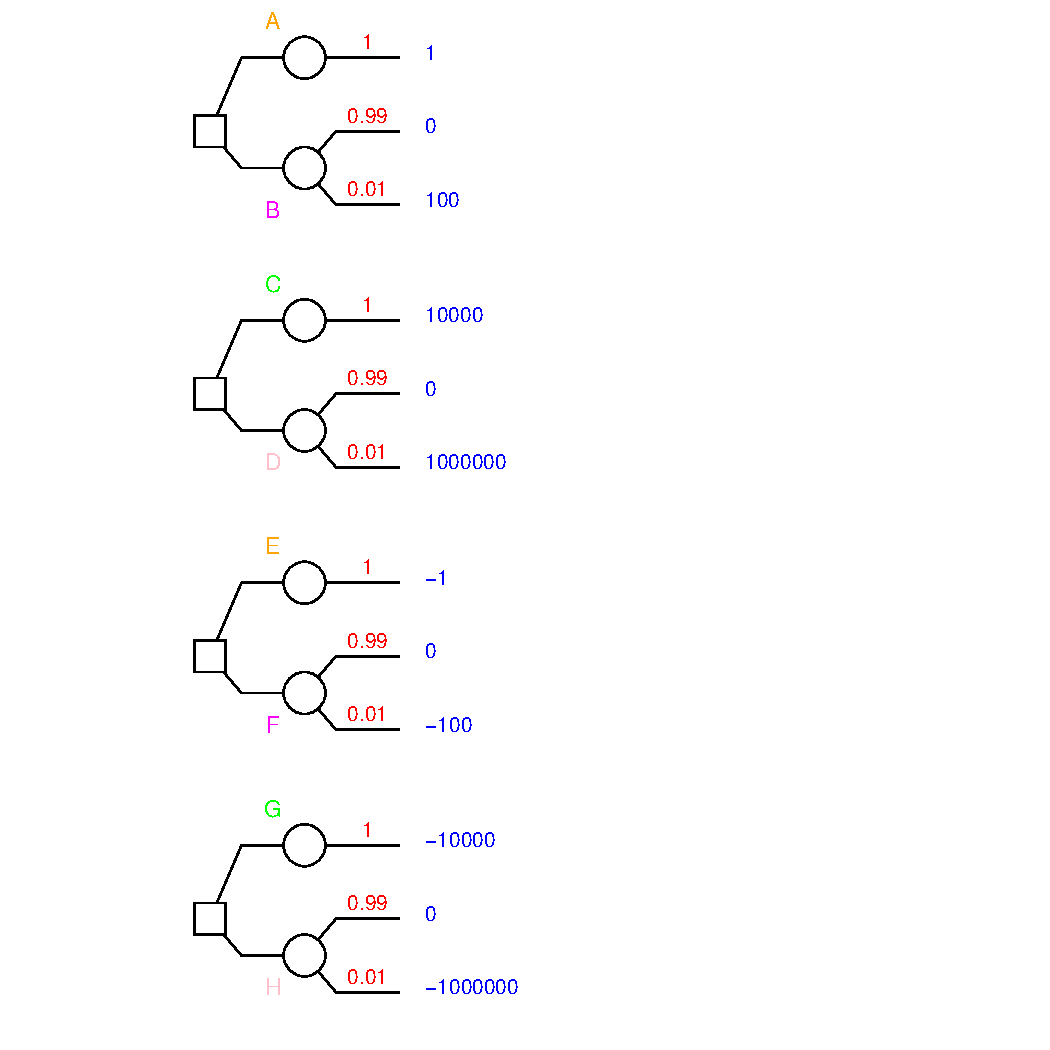
\includegraphics[width=0.8\linewidth]{figure/unnamed-chunk-34} 

}



\end{knitrout}


A sample of $36$ people were asked to consider the first choice between gambles $A$ and $B$, with
$81\%$ choosing the risky option $B$ (see \cite[][p. 406 Table 3, Experiment 1, Question 13]{Hershey_Schoemaker_1980}). For small outcome gains, people were risk seeking.
In the second choice situation between gambles $C$ and $D$, $88\%$ of $37$ people chose $C$, the safe
option. For large outcome gains, people were risk averse.
In the third choice situation between gambles $E$ and $F$, $63\%$ of $36$ people chose $E$, the safe
option. For small outcome losses, people were risk averse.
Finally, in the fourth choice situation between gambles $G$ and $H$, $68\%$ of $37$ people chose $H$, the risky option. For large outcome losses, people were risk seeking.
The PT predictions using parameterisations from \citet[][]{Scholten_Read_2014} can be calculated as follows.

\begin{knitrout}
\definecolor{shadecolor}{rgb}{0.969, 0.969, 0.969}\color{fgcolor}\begin{kframe}
\begin{alltt}
\hlstd{norm_log_utility} \hlkwb{<-} \hlkwd{Utility}\hlstd{(}\hlkwc{fun}\hlstd{=}\hlstr{"normalized_logarithmic"}\hlstd{,} \hlkwc{par}\hlstd{=}\hlkwd{c}\hlstd{(}\hlkwc{alpha}\hlstd{=}\hlnum{0.032}\hlstd{,} \hlkwc{beta}\hlstd{=}\hlnum{0.0031}\hlstd{,} \hlkwc{lambda}\hlstd{=}\hlnum{2.25}\hlstd{))}
\hlstd{tk_1992_positive_prob_weight} \hlkwb{<-} \hlkwd{ProbWeight}\hlstd{(}\hlkwc{fun}\hlstd{=}\hlstr{"Tversky_Kahneman_1992"}\hlstd{,} \hlkwc{par}\hlstd{=}\hlkwd{c}\hlstd{(}\hlkwc{alpha}\hlstd{=}\hlnum{0.4496}\hlstd{))}
\hlstd{tk_1992_negative_prob_weight} \hlkwb{<-} \hlkwd{ProbWeight}\hlstd{(}\hlkwc{fun}\hlstd{=}\hlstr{"Tversky_Kahneman_1992"}\hlstd{,} \hlkwc{par}\hlstd{=}\hlkwd{c}\hlstd{(}\hlkwc{alpha}\hlstd{=}\hlnum{0.6704}\hlstd{))}
\hlkwd{comparePT}\hlstd{(my_choices,}
        \hlkwc{prob_weight_for_positive_outcomes}\hlstd{=tk_1992_positive_prob_weight,}
        \hlkwc{prob_weight_for_negative_outcomes}\hlstd{=tk_1992_negative_prob_weight,}
        \hlkwc{utility}\hlstd{=norm_log_utility,} \hlkwc{digits}\hlstd{=}\hlnum{4}\hlstd{)}
\end{alltt}
\begin{verbatim}
##   cid gid     ev     pt    ce     rp
## 1   1   1      1 0.9843 11.86 -10.86
## 2   1   2      1  4.382 13.23 -12.23
## 3   2   1  10000  180.4  3690   6310
## 4   2   2  10000  31.67 31.68   9968
## 5   3   1     -1 -2.247     1     -2
## 6   3   2     -1 -8.447 3.776 -4.776
## 7   4   1 -10000  -2515 10000 -20000
## 8   4   2 -10000 -251.5 133.6 -10134
\end{verbatim}
\end{kframe}
\end{knitrout}


The predicted preferences are $B > A$, $C > D$, $E > F$ and $H > G$, in line with the empirical data.

\section{Loss aversion}

\citet[][p. 466]{Birnbaum_2008} defines loss aversion as ``the behavioral finding that people show risk
aversion for mixed gambles".
Prospect theory explains loss aversion through a kinked utility function centred around a reference point (which usually but not always represents the status quo).
This construct underpins the famous quote from \citet[][p. 279]{Kahneman_Tversky_1979} that ``losses loom larger than gains". It extends the EU utility function into the domain of losses and embodies the conceptual advance that decision makers consider changes in wealth states
relative to the reference point of their current wealth (rather than only final wealth states), developing a line of thought from \cite{Markowitz_1952}. \citet[][p. 269-277]{Kahneman_2011} offers an account of how this idea came about.

Consider the choice from \citet[][Table 5 p. 221]{Erev_2013} consisting of the option of maintaining the status quo or the option of taking a symmetrical gamble where the absolute value of the loss is the same as the gain. Assume the units of the gambles are of high nominal value and that real money is involved. {\bf pt} can model this choice.

\begin{knitrout}
\definecolor{shadecolor}{rgb}{0.969, 0.969, 0.969}\color{fgcolor}\begin{kframe}
\begin{alltt}
\hlstd{choice_ids} \hlkwb{<-} \hlkwd{c}\hlstd{(}\hlnum{1}\hlstd{,} \hlnum{1}\hlstd{,} \hlnum{1}\hlstd{)}
\hlstd{gamble_ids} \hlkwb{<-} \hlkwd{c}\hlstd{(}\hlnum{1}\hlstd{,} \hlnum{2}\hlstd{,} \hlnum{2}\hlstd{)}
\hlstd{outcome_ids} \hlkwb{<-} \hlkwd{c}\hlstd{(}\hlnum{1}\hlstd{,} \hlnum{1}\hlstd{,} \hlnum{2}\hlstd{)}
\hlstd{objective_consequences} \hlkwb{<-} \hlkwd{c}\hlstd{(}\hlnum{0}\hlstd{,} \hlopt{-}\hlnum{100}\hlstd{,} \hlnum{100}\hlstd{)}
\hlstd{probability_strings} \hlkwb{<-} \hlkwd{c}\hlstd{(}\hlstr{"1"}\hlstd{,} \hlstr{"1/2"}\hlstd{,} \hlstr{"1/2"}\hlstd{)}
\hlstd{my_choices} \hlkwb{<-} \hlkwd{Choices}\hlstd{(}\hlkwc{choice_ids}\hlstd{=choice_ids,}
        \hlkwc{gamble_ids}\hlstd{=gamble_ids,}
        \hlkwc{outcome_ids}\hlstd{=outcome_ids,}
        \hlkwc{objective_consequences}\hlstd{=objective_consequences,}
        \hlkwc{probability_strings}\hlstd{=probability_strings)}
\hlstd{my_choices}
\end{alltt}
\begin{verbatim}
##   cid gid oid  pr   oc
## 1   1   1   1   1    0
## 2   1   2   1 1/2 -100
## 3   1   2   2 1/2  100
\end{verbatim}
\begin{alltt}
\hlkwd{drawChoices}\hlstd{(my_choices,}
        \hlkwc{decision_square_x}\hlstd{=}\hlnum{0.2}\hlstd{,} \hlkwc{decision_square_edge_length}\hlstd{=}\hlnum{0.05}\hlstd{,}
        \hlkwc{circle_radius}\hlstd{=}\hlnum{0.025}\hlstd{,} \hlkwc{y_split_gap}\hlstd{=}\hlnum{0.15}\hlstd{,} \hlkwc{x_split_offset}\hlstd{=}\hlnum{0.03}\hlstd{,}
        \hlkwc{probability_text_digits}\hlstd{=}\hlnum{4}\hlstd{,} \hlkwc{y_probability_text_offset}\hlstd{=}\hlnum{0.015}\hlstd{,}
        \hlkwc{y_value_text_offset}\hlstd{=}\hlnum{0.005}\hlstd{,} \hlkwc{x_value_text_offset}\hlstd{=}\hlnum{0.025}\hlstd{,}
        \hlkwc{probability_text_font_colour}\hlstd{=}\hlstr{"red"}\hlstd{,} \hlkwc{probability_text_font_size}\hlstd{=}\hlnum{10}\hlstd{,}
        \hlkwc{objective_consequence_text_font_colour}\hlstd{=}\hlstr{"blue"}\hlstd{,}
        \hlkwc{objective_consequence_text_font_size}\hlstd{=}\hlnum{10}\hlstd{,} \hlkwc{label}\hlstd{=}\hlkwd{c}\hlstd{(}\hlstr{"A"}\hlstd{,}\hlstr{"B"}\hlstd{),}
        \hlkwc{label_font_colour}\hlstd{=}\hlkwd{c}\hlstd{(}\hlstr{"orange"}\hlstd{,}\hlstr{"magenta"}\hlstd{),} \hlkwc{label_font_size}\hlstd{=}\hlkwd{c}\hlstd{(}\hlnum{11}\hlstd{,}\hlnum{11}\hlstd{),}
        \hlkwc{label_positions}\hlstd{=}\hlkwd{list}\hlstd{(}\hlkwd{c}\hlstd{(}\hlnum{0.26}\hlstd{,}\hlnum{0.7}\hlstd{),}\hlkwd{c}\hlstd{(}\hlnum{0.26}\hlstd{,}\hlnum{0.36}\hlstd{)))}
\end{alltt}
\end{kframe}

{\centering 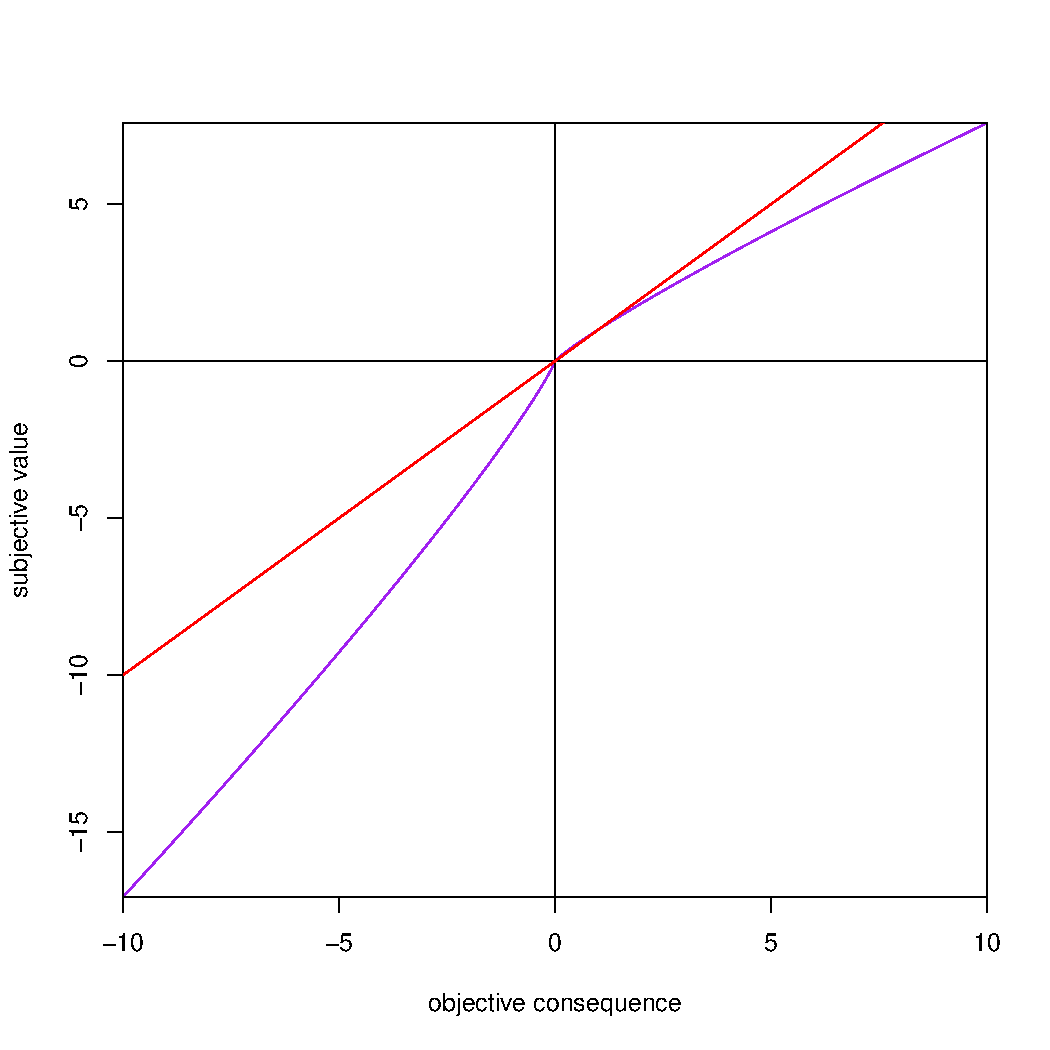
\includegraphics[width=0.8\linewidth]{figure/unnamed-chunk-36} 

}



\end{knitrout}


In the \cite{Erev_2013} study, $88\%$ of the $46$ undergraduate students respondents in the study were risk averse and chose the status quo, supporting prospect theory's absolute loss aversion
hypothesis. There is further empirical support for this phenomenon \citep[see, e.g.][]{Brooks_Zank_2005, Birnbaum_Bahra_2007, Ert_Erev_2008,  McGraw_Larsen_Kahneman_Schkade_2010, Redelmeier_Tversky_1992}. However, a number of experimental manipulations such as introducing the presence of status quo framing effects seem to enhance its presence \citep*{Erev_2013}. \cite{Rabin_2000} provided a proof that with the assumption of a concave utility function, an expected utility maximizer would reject an extremely favourable $50-50$ gamble with large nominal value (e.g. $(-100, 0.5; 2.5 \times 10^9, 0.5)$) if they rejected a $50-50$ gamble with small nominal value (e.g. $(-100, 0.5; 110, 0.5)$). \cite{Rabin_Thaler_2001} suggests a combination of loss aversion and mental accounting explains risk averse behaviour for small nominal value gambles rather than expected utility.
From an evolutionary psychology perspective, \cite{de_Martino_Camerer_Adolphs_Purves_2010} suggest the amygdala regulates loss aversion.

\cite{Erev_2013} tabled the loss aversion coefficient $\lambda$ across a number of studies such as \cite{Kobberling_Wakker_2005, Abdellaoui_Bleichrodt_Paraschiv_2007}, and found it fell within in the range $[0.78, 2.61]$,
with a strong positive correlation between the magnitude of $\lambda$ and the absolute value of the
objective consequences. Expressed very roughly, decision makers require gains to be at least twice the absolute value of the losses in an equal chance binary gamble before they will consider taking on the gamble \cite[see][p. 1053-1054]{Tversky_Kahneman_1991}. Calculations for PT can be performed via the following code.

\begin{knitrout}
\definecolor{shadecolor}{rgb}{0.969, 0.969, 0.969}\color{fgcolor}\begin{kframe}
\begin{alltt}
\hlstd{tk_1992_utility} \hlkwb{<-} \hlkwd{Utility}\hlstd{(}\hlkwc{fun}\hlstd{=}\hlstr{"power"}\hlstd{,} \hlkwc{par}\hlstd{=}\hlkwd{c}\hlstd{(}\hlkwc{alpha}\hlstd{=}\hlnum{0.88}\hlstd{,} \hlkwc{beta}\hlstd{=}\hlnum{0.88}\hlstd{,} \hlkwc{lambda}\hlstd{=}\hlnum{2.25}\hlstd{))}
\hlstd{linear_in_log_odds_prob_weight} \hlkwb{<-} \hlkwd{ProbWeight}\hlstd{(}\hlkwc{fun}\hlstd{=}\hlstr{"linear_in_log_odds"}\hlstd{,} \hlkwc{par}\hlstd{=}\hlkwd{c}\hlstd{(}\hlkwc{alpha}\hlstd{=}\hlnum{0.61}\hlstd{,} \hlkwc{beta}\hlstd{=}\hlnum{0.724}\hlstd{))}
\hlkwd{comparePT}\hlstd{(my_choices,}
        \hlkwc{prob_weight_for_positive_outcomes}\hlstd{=linear_in_log_odds_prob_weight,}
        \hlkwc{prob_weight_for_negative_outcomes}\hlstd{=linear_in_log_odds_prob_weight,}
        \hlkwc{utility}\hlstd{=tk_1992_utility,} \hlkwc{digits}\hlstd{=}\hlnum{4}\hlstd{)}
\end{alltt}
\begin{verbatim}
##   cid gid ev     pt     ce    rp
## 1   1   1  0      0      0     0
## 2   1   2  0 -30.21 -19.13 19.13
\end{verbatim}
\end{kframe}
\end{knitrout}


Prospect theory gives a negative value of $-30.2$ for gamble $B$, less than the $0$ of the certain gamble $A$. Thus
the riskless choice is preferred.
Note that loss aversion can be explained by other theories such as TAX, without the use of a kinked utility
function \citep*{Birnbaum_2006}. In the following example a linear utility function is used in the TAX calculation. In the internal calculations for TAX, branch weights of $2/3$ and
$1/3$ are given to the $-100$ and $100$ outcomes, respectively.

\begin{knitrout}
\definecolor{shadecolor}{rgb}{0.969, 0.969, 0.969}\color{fgcolor}\begin{kframe}
\begin{alltt}
\hlstd{my_utility} \hlkwb{<-} \hlkwd{Utility}\hlstd{(}\hlkwc{fun}\hlstd{=}\hlstr{"linear"}\hlstd{,} \hlkwc{par}\hlstd{=}\hlkwd{c}\hlstd{(}\hlkwc{lambda}\hlstd{=}\hlnum{1}\hlstd{))}
\hlstd{power_prob_weight} \hlkwb{<-} \hlkwd{ProbWeight}\hlstd{(}\hlkwc{fun}\hlstd{=}\hlstr{"power"}\hlstd{,} \hlkwc{par}\hlstd{=}\hlkwd{c}\hlstd{(}\hlkwc{alpha}\hlstd{=}\hlnum{0.7}\hlstd{,} \hlkwc{beta}\hlstd{=}\hlnum{1}\hlstd{))}
\hlkwd{compareTAX}\hlstd{(my_choices,} \hlkwc{prob_weight}\hlstd{=power_prob_weight,} \hlkwc{utility}\hlstd{=my_utility,} \hlkwc{delta}\hlstd{=}\hlopt{-}\hlnum{1}\hlstd{,} \hlkwc{digits}\hlstd{=}\hlnum{4}\hlstd{)}
\end{alltt}
\begin{verbatim}
##   cid gid ev    tax     ce    rp
## 1   1   1  0      0      0     0
## 2   1   2  0 -33.33 -33.33 33.33
\end{verbatim}
\end{kframe}
\end{knitrout}


The value is $-33.3$ for gamble $B$, less than the $0$ of gamble $A$. Thus the riskless choice is preferred as well.

\section{Critical tests of prospect theory}

PT assumes transitivity, coalescing, first-order stochastic dominance, restricted branch independence,
upper tail independence, lower cumulative independence, upper cumulative independence and gain-loss separability \citep*{Birnbaum_2008}.
However, empirical research has detected violations of some of these assumptions to various extents. Violations of gain-loss separability and coalescing will first be discussed as these seem fundamental issues. Violations of first-order stochastic dominance will also be discussed to demonstrate the implementation of the \citet[][p. 74]{Birnbaum_1997} stochastic dominance violation recipe in {\bf pt}.

\subsection{Violations of gain-loss separability}

A PT assumption is the separability of gains and losses, implicit in the kinked shape of the utility function around a reference point.
The PT utility function of Eq. \eqref{pt_utility_function} can be plotted as follows.

\begin{knitrout}
\definecolor{shadecolor}{rgb}{0.969, 0.969, 0.969}\color{fgcolor}\begin{kframe}
\begin{alltt}
\hlkwd{plotUtility}\hlstd{(}\hlkwc{my_x_label} \hlstd{=} \hlstr{"objective consequence"}\hlstd{,}
        \hlkwc{my_y_label} \hlstd{=} \hlstr{"subjective value"}\hlstd{,}
        \hlkwc{xmin} \hlstd{=} \hlopt{-}\hlnum{10}\hlstd{,} \hlkwc{xmax} \hlstd{=} \hlnum{10}\hlstd{,} \hlkwc{fun}\hlstd{=power_uf,}
        \hlkwc{par}\hlstd{=}\hlkwd{c}\hlstd{(}\hlkwc{alpha} \hlstd{=} \hlnum{0.88}\hlstd{,} \hlkwc{beta} \hlstd{=} \hlnum{0.88}\hlstd{,} \hlkwc{lambda} \hlstd{=} \hlnum{2.25}\hlstd{),}
        \hlkwc{fun_colour} \hlstd{=} \hlstr{"purple"}\hlstd{,}
        \hlkwc{draw_reference_line_flag} \hlstd{=} \hlnum{TRUE}\hlstd{,}
        \hlkwc{reference_line_colour} \hlstd{=} \hlstr{"red"}\hlstd{,}
        \hlkwc{reference_line_style} \hlstd{=} \hlnum{1}\hlstd{)}
\end{alltt}
\end{kframe}

{\centering 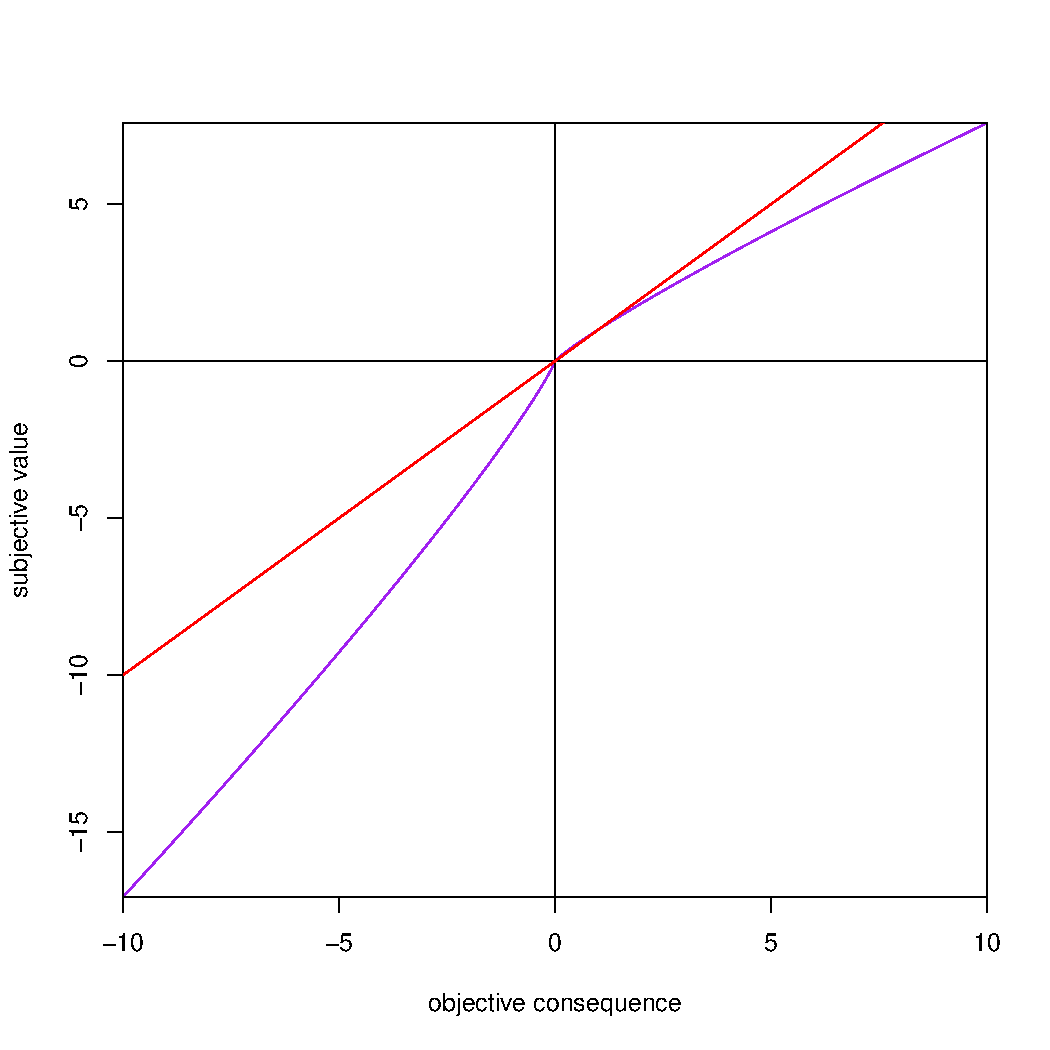
\includegraphics[width=0.8\linewidth]{figure/unnamed-chunk-39} 

}



\end{knitrout}


At present very little empirical research has been conducted on gain-loss separability. The limited research available has generated evidence where gain-loss separability is violated \citep*{Birnbaum_Bahra_2007, Wu_Markle_2008, Por_Budescu_2013}. Consider tests 15, 13 and 11 from \citet[][Table 4 p. 1021]{Birnbaum_Bahra_2007}.

\begin{knitrout}
\definecolor{shadecolor}{rgb}{0.969, 0.969, 0.969}\color{fgcolor}\begin{kframe}
\begin{alltt}
\hlstd{choice_ids} \hlkwb{<-} \hlkwd{c}\hlstd{(}\hlnum{1}\hlstd{,} \hlnum{1}\hlstd{,} \hlnum{1}\hlstd{,} \hlnum{1}\hlstd{,} \hlnum{1}\hlstd{,} \hlnum{1}\hlstd{,} \hlnum{2}\hlstd{,} \hlnum{2}\hlstd{,} \hlnum{2}\hlstd{,} \hlnum{2}\hlstd{,} \hlnum{2}\hlstd{,} \hlnum{2}\hlstd{,} \hlnum{3}\hlstd{,} \hlnum{3}\hlstd{,} \hlnum{3}\hlstd{,} \hlnum{3}\hlstd{,} \hlnum{3}\hlstd{,} \hlnum{3}\hlstd{)}
\hlstd{gamble_ids} \hlkwb{<-} \hlkwd{c}\hlstd{(}\hlnum{1}\hlstd{,} \hlnum{1}\hlstd{,} \hlnum{1}\hlstd{,} \hlnum{2}\hlstd{,} \hlnum{2}\hlstd{,} \hlnum{2}\hlstd{,} \hlnum{1}\hlstd{,} \hlnum{1}\hlstd{,} \hlnum{1}\hlstd{,} \hlnum{2}\hlstd{,} \hlnum{2}\hlstd{,} \hlnum{2}\hlstd{,} \hlnum{1}\hlstd{,} \hlnum{1}\hlstd{,} \hlnum{1}\hlstd{,} \hlnum{2}\hlstd{,} \hlnum{2}\hlstd{,} \hlnum{2}\hlstd{)}
\hlstd{outcome_ids} \hlkwb{<-} \hlkwd{c}\hlstd{(}\hlnum{1}\hlstd{,} \hlnum{2}\hlstd{,} \hlnum{3}\hlstd{,} \hlnum{1}\hlstd{,} \hlnum{2}\hlstd{,} \hlnum{3}\hlstd{,} \hlnum{1}\hlstd{,} \hlnum{2}\hlstd{,} \hlnum{3}\hlstd{,} \hlnum{1}\hlstd{,} \hlnum{2}\hlstd{,} \hlnum{3}\hlstd{,} \hlnum{1}\hlstd{,} \hlnum{2}\hlstd{,} \hlnum{3}\hlstd{,} \hlnum{1}\hlstd{,} \hlnum{2}\hlstd{,} \hlnum{3}\hlstd{)}
\hlstd{objective_consequences} \hlkwb{<-} \hlkwd{c}\hlstd{(}\hlnum{100}\hlstd{,} \hlnum{0}\hlstd{,} \hlnum{0}\hlstd{,} \hlnum{50}\hlstd{,} \hlnum{50}\hlstd{,} \hlnum{0}\hlstd{,}
        \hlopt{-}\hlnum{0}\hlstd{,} \hlopt{-}\hlnum{50}\hlstd{,} \hlopt{-}\hlnum{50}\hlstd{,} \hlopt{-}\hlnum{0}\hlstd{,} \hlopt{-}\hlnum{0}\hlstd{,} \hlopt{-}\hlnum{100}\hlstd{,}
        \hlnum{100}\hlstd{,} \hlnum{0}\hlstd{,} \hlopt{-}\hlnum{50}\hlstd{,} \hlnum{50}\hlstd{,} \hlopt{-}\hlnum{0}\hlstd{,} \hlopt{-}\hlnum{100}\hlstd{)}
\hlstd{probability_strings} \hlkwb{<-} \hlkwd{c}\hlstd{(}\hlstr{"0.25"}\hlstd{,} \hlstr{"0.25"}\hlstd{,} \hlstr{"0.5"}\hlstd{,} \hlstr{"0.25"}\hlstd{,} \hlstr{"0.25"}\hlstd{,} \hlstr{"0.5"}\hlstd{,}
        \hlstr{"0.5"}\hlstd{,} \hlstr{"0.25"}\hlstd{,} \hlstr{"0.25"}\hlstd{,} \hlstr{"0.5"}\hlstd{,} \hlstr{"0.25"}\hlstd{,} \hlstr{"0.25"}\hlstd{,}
        \hlstr{"0.25"}\hlstd{,} \hlstr{"0.25"}\hlstd{,} \hlstr{"0.5"}\hlstd{,} \hlstr{"0.5"}\hlstd{,} \hlstr{"0.25"}\hlstd{,} \hlstr{"0.25"}\hlstd{)}
\hlstd{my_choices} \hlkwb{<-} \hlkwd{Choices}\hlstd{(}\hlkwc{choice_ids}\hlstd{=choice_ids,}
        \hlkwc{gamble_ids}\hlstd{=gamble_ids,}
        \hlkwc{outcome_ids}\hlstd{=outcome_ids,}
        \hlkwc{objective_consequences}\hlstd{=objective_consequences,}
        \hlkwc{probability_strings}\hlstd{=probability_strings)}
\hlstd{my_choices}
\end{alltt}
\begin{verbatim}
##    cid gid oid   pr   oc
## 1    1   1   1 0.25  100
## 2    1   1   2 0.25    0
## 3    1   1   3  0.5    0
## 4    1   2   1 0.25   50
## 5    1   2   2 0.25   50
## 6    1   2   3  0.5    0
## 7    2   1   1  0.5    0
## 8    2   1   2 0.25  -50
## 9    2   1   3 0.25  -50
## 10   2   2   1  0.5    0
## 11   2   2   2 0.25    0
## 12   2   2   3 0.25 -100
## 13   3   1   1 0.25  100
## 14   3   1   2 0.25    0
## 15   3   1   3  0.5  -50
## 16   3   2   1  0.5   50
## 17   3   2   2 0.25    0
## 18   3   2   3 0.25 -100
\end{verbatim}
\begin{alltt}
\hlkwd{drawChoices}\hlstd{(my_choices,}
        \hlkwc{decision_square_x}\hlstd{=}\hlnum{0.2}\hlstd{,} \hlkwc{decision_square_edge_length}\hlstd{=}\hlnum{0.03}\hlstd{,}
        \hlkwc{circle_radius}\hlstd{=}\hlnum{0.02}\hlstd{,} \hlkwc{y_split_gap}\hlstd{=}\hlnum{0.04}\hlstd{,} \hlkwc{x_split_offset}\hlstd{=}\hlnum{0.03}\hlstd{,}
        \hlkwc{probability_text_digits}\hlstd{=}\hlnum{4}\hlstd{,} \hlkwc{y_probability_text_offset}\hlstd{=}\hlnum{0.015}\hlstd{,}
        \hlkwc{y_value_text_offset}\hlstd{=}\hlnum{0.005}\hlstd{,} \hlkwc{x_value_text_offset}\hlstd{=}\hlnum{0.025}\hlstd{,}
        \hlkwc{probability_text_font_colour}\hlstd{=}\hlstr{"red"}\hlstd{,} \hlkwc{probability_text_font_size}\hlstd{=}\hlnum{10}\hlstd{,}
        \hlkwc{objective_consequence_text_font_colour}\hlstd{=}\hlstr{"blue"}\hlstd{,}
        \hlkwc{objective_consequence_text_font_size}\hlstd{=}\hlnum{10}\hlstd{,}
        \hlkwc{label}\hlstd{=}\hlkwd{c}\hlstd{(}\hlstr{"A"}\hlstd{,}\hlstr{"B"}\hlstd{,}\hlstr{"C"}\hlstd{,} \hlstr{"D"}\hlstd{,}\hlstr{"E"}\hlstd{,}\hlstr{"F"}\hlstd{),}
        \hlkwc{label_font_colour}\hlstd{=}\hlkwd{c}\hlstd{(}\hlstr{"orange"}\hlstd{,}\hlstr{"magenta"}\hlstd{,}\hlstr{"green"}\hlstd{,}
                \hlstr{"blue"}\hlstd{,}\hlstr{"purple"}\hlstd{,}\hlstr{"pink"}\hlstd{),}
        \hlkwc{label_font_size}\hlstd{=}\hlkwd{c}\hlstd{(}\hlnum{11}\hlstd{,}\hlnum{11}\hlstd{,}\hlnum{11}\hlstd{,}\hlnum{11}\hlstd{,}\hlnum{11}\hlstd{,}\hlnum{11}\hlstd{),}
        \hlkwc{label_positions}\hlstd{=}\hlkwd{list}\hlstd{(}\hlkwd{c}\hlstd{(}\hlnum{0.26}\hlstd{,}\hlnum{0.93}\hlstd{),}\hlkwd{c}\hlstd{(}\hlnum{0.26}\hlstd{,}\hlnum{0.74}\hlstd{),}
                \hlkwd{c}\hlstd{(}\hlnum{0.26}\hlstd{,}\hlnum{0.6}\hlstd{),}\hlkwd{c}\hlstd{(}\hlnum{0.26}\hlstd{,}\hlnum{0.4}\hlstd{),}\hlkwd{c}\hlstd{(}\hlnum{0.26}\hlstd{,}\hlnum{0.28}\hlstd{),}\hlkwd{c}\hlstd{(}\hlnum{0.26}\hlstd{,}\hlnum{0.05}\hlstd{)))}
\end{alltt}
\end{kframe}

{\centering 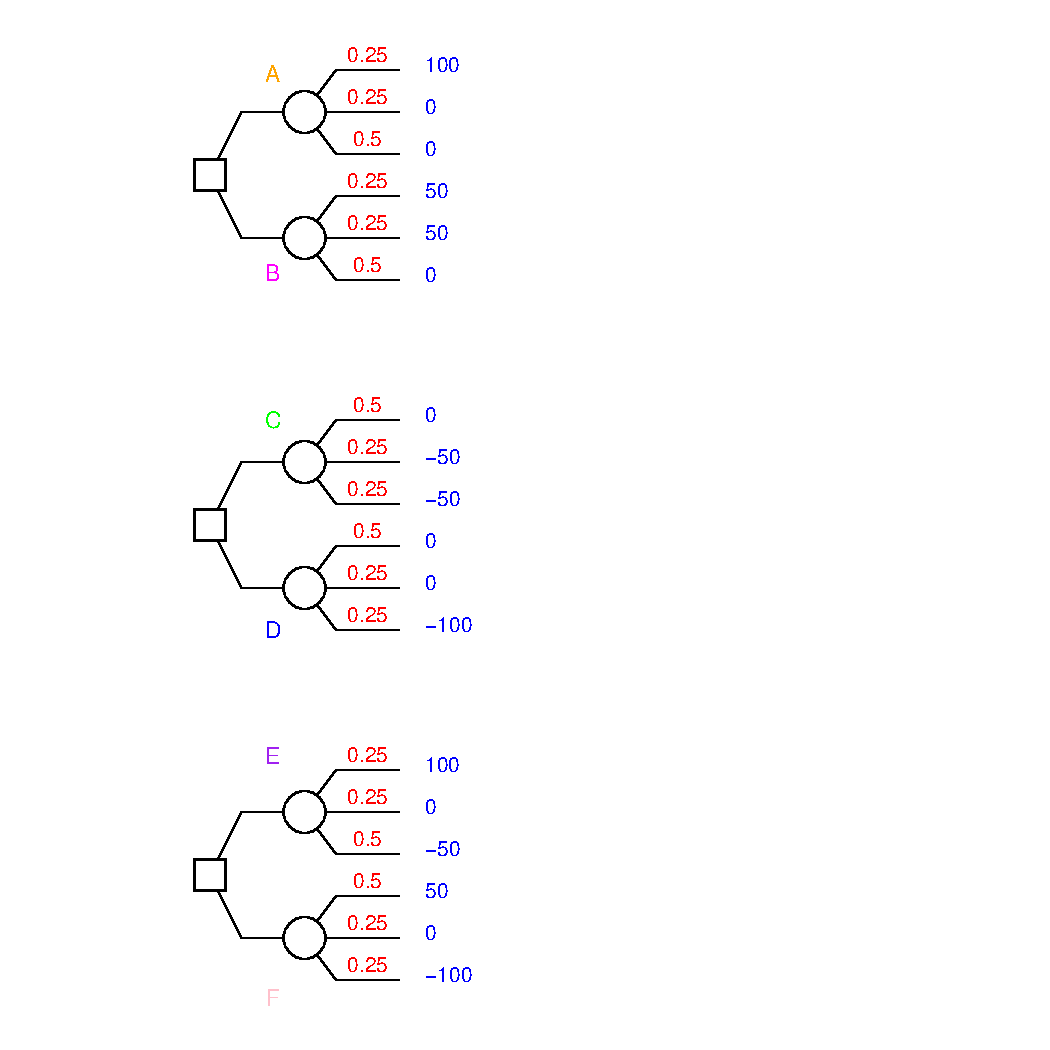
\includegraphics[width=0.8\linewidth]{figure/unnamed-chunk-40} 

}



\end{knitrout}


In a sample of $178$ participants $71\%$ preferred $B > A$, $65\%$ preferred $D > C$ and $76\%$ preferred $E > F$. The calculations for PT can be run as follows.

\begin{knitrout}
\definecolor{shadecolor}{rgb}{0.969, 0.969, 0.969}\color{fgcolor}\begin{kframe}
\begin{alltt}
\hlstd{tk_1992_utility} \hlkwb{<-} \hlkwd{Utility}\hlstd{(}\hlkwc{fun}\hlstd{=}\hlstr{"power"}\hlstd{,} \hlkwc{par}\hlstd{=}\hlkwd{c}\hlstd{(}\hlkwc{alpha}\hlstd{=}\hlnum{0.88}\hlstd{,} \hlkwc{beta}\hlstd{=}\hlnum{0.88}\hlstd{,} \hlkwc{lambda}\hlstd{=}\hlnum{2.25}\hlstd{))}
\hlstd{tk_1992_positive_prob_weight} \hlkwb{<-} \hlkwd{ProbWeight}\hlstd{(}\hlkwc{fun}\hlstd{=}\hlstr{"Tversky_Kahneman_1992"}\hlstd{,} \hlkwc{par}\hlstd{=}\hlkwd{c}\hlstd{(}\hlkwc{alpha}\hlstd{=}\hlnum{0.61}\hlstd{))}
\hlstd{tk_1992_negative_prob_weight} \hlkwb{<-} \hlkwd{ProbWeight}\hlstd{(}\hlkwc{fun}\hlstd{=}\hlstr{"Tversky_Kahneman_1992"}\hlstd{,} \hlkwc{par}\hlstd{=}\hlkwd{c}\hlstd{(}\hlkwc{alpha}\hlstd{=}\hlnum{0.69}\hlstd{))}
\hlkwd{comparePT}\hlstd{(my_choices,}
        \hlkwc{prob_weight_for_positive_outcomes}\hlstd{=tk_1992_positive_prob_weight,}
        \hlkwc{prob_weight_for_negative_outcomes}\hlstd{=tk_1992_negative_prob_weight,}
        \hlkwc{utility}\hlstd{=tk_1992_utility,} \hlkwc{digits}\hlstd{=}\hlnum{4}\hlstd{)}
\end{alltt}
\begin{verbatim}
##   cid gid  ev     pt     ce      rp
## 1   1   1  25  16.73  24.57   0.433
## 2   1   2  25  13.15  18.69   6.311
## 3   2   1 -25 -31.94 -20.38  -4.618
## 4   2   2 -25    -38 -24.83 -0.1664
## 5   3   1   0 -15.21 -8.771   8.771
## 6   3   2   0 -24.85 -15.33   15.33
\end{verbatim}
\end{kframe}
\end{knitrout}


PT incorrectly predicts the preferences $A > B$ and $C > D$ but correctly predicts $E > F$.
\cite{Por_Budescu_2013} suggest violations of gain-loss separability could limit the ability of PT to generalise from purely positive or negative domain gambles to mixed gambles.

In contrast, TAX explains loss aversion through the increased weighting provided to negative choice branches
rather than through using a kinked utility function. Note the linear utility $u(x) = x$ and loss aversion coefficient $\lambda = 1$ used in the following TAX calculation.

\begin{knitrout}
\definecolor{shadecolor}{rgb}{0.969, 0.969, 0.969}\color{fgcolor}\begin{kframe}
\begin{alltt}
\hlstd{my_utility} \hlkwb{<-} \hlkwd{Utility}\hlstd{(}\hlkwc{fun}\hlstd{=}\hlstr{"linear"}\hlstd{,} \hlkwc{par}\hlstd{=}\hlkwd{c}\hlstd{(}\hlkwc{lambda}\hlstd{=}\hlnum{1}\hlstd{))}
\hlstd{power_prob_weight} \hlkwb{<-} \hlkwd{ProbWeight}\hlstd{(}\hlkwc{fun}\hlstd{=}\hlstr{"power"}\hlstd{,} \hlkwc{par}\hlstd{=}\hlkwd{c}\hlstd{(}\hlkwc{alpha}\hlstd{=}\hlnum{0.7}\hlstd{,} \hlkwc{beta}\hlstd{=}\hlnum{1}\hlstd{))}
\hlkwd{compareTAX}\hlstd{(my_choices,} \hlkwc{prob_weight}\hlstd{=power_prob_weight,} \hlkwc{utility}\hlstd{=my_utility,} \hlkwc{delta}\hlstd{=}\hlopt{-}\hlnum{1}\hlstd{,} \hlkwc{digits}\hlstd{=}\hlnum{4}\hlstd{)}
\end{alltt}
\begin{verbatim}
##   cid gid  ev    tax     ce     rp
## 1   1   1  25  13.79  13.79  11.21
## 2   1   2  25  20.69  20.69  4.308
## 3   2   1 -25 -20.69 -20.69 -4.308
## 4   2   2 -25 -13.79 -13.79 -11.21
## 5   3   1   0 -15.51 -15.51  15.51
## 6   3   2   0 -34.49 -34.49  34.49
\end{verbatim}
\end{kframe}
\end{knitrout}


In this case TAX successfully predicts $B > A$, $D > C$ and $E > F$, in line with the empirical results.
However, this is not true for other cases.
Consider test 7 from \citet[][Table 1 p. 1326]{Wu_Markle_2008}. These choices can be modelled as follows.

\begin{knitrout}
\definecolor{shadecolor}{rgb}{0.969, 0.969, 0.969}\color{fgcolor}\begin{kframe}
\begin{alltt}
\hlstd{choice_ids} \hlkwb{<-} \hlkwd{c}\hlstd{(}\hlnum{1}\hlstd{,} \hlnum{1}\hlstd{,} \hlnum{1}\hlstd{,} \hlnum{1}\hlstd{,} \hlnum{2}\hlstd{,} \hlnum{2}\hlstd{,} \hlnum{2}\hlstd{,} \hlnum{2}\hlstd{,} \hlnum{3}\hlstd{,} \hlnum{3}\hlstd{,} \hlnum{3}\hlstd{,} \hlnum{3}\hlstd{)}
\hlstd{gamble_ids} \hlkwb{<-} \hlkwd{c}\hlstd{(}\hlnum{1}\hlstd{,} \hlnum{1}\hlstd{,} \hlnum{2}\hlstd{,} \hlnum{2}\hlstd{,} \hlnum{1}\hlstd{,} \hlnum{1}\hlstd{,} \hlnum{2}\hlstd{,} \hlnum{2}\hlstd{,} \hlnum{1}\hlstd{,} \hlnum{1}\hlstd{,} \hlnum{2}\hlstd{,} \hlnum{2}\hlstd{)}
\hlstd{outcome_ids} \hlkwb{<-} \hlkwd{c}\hlstd{(}\hlnum{1}\hlstd{,} \hlnum{2}\hlstd{,} \hlnum{1}\hlstd{,} \hlnum{2}\hlstd{,} \hlnum{1}\hlstd{,} \hlnum{2}\hlstd{,} \hlnum{1}\hlstd{,} \hlnum{2}\hlstd{,} \hlnum{1}\hlstd{,} \hlnum{2}\hlstd{,} \hlnum{1}\hlstd{,} \hlnum{2}\hlstd{)}
\hlstd{objective_consequences} \hlkwb{<-} \hlkwd{c}\hlstd{(}\hlnum{4200}\hlstd{,} \hlopt{-}\hlnum{3000}\hlstd{,} \hlnum{3000}\hlstd{,} \hlopt{-}\hlnum{6000}\hlstd{,}
        \hlnum{4200}\hlstd{,} \hlnum{0}\hlstd{,} \hlnum{3000}\hlstd{,} \hlnum{0}\hlstd{,}
        \hlnum{0}\hlstd{,} \hlopt{-}\hlnum{3000}\hlstd{,} \hlnum{0}\hlstd{,} \hlopt{-}\hlnum{6000}\hlstd{)}
\hlstd{probability_strings} \hlkwb{<-} \hlkwd{c}\hlstd{(}\hlstr{"0.5"}\hlstd{,} \hlstr{"0.5"}\hlstd{,} \hlstr{"0.75"}\hlstd{,} \hlstr{"0.25"}\hlstd{,}
        \hlstr{"0.5"}\hlstd{,} \hlstr{"0.5"}\hlstd{,} \hlstr{"0.75"}\hlstd{,} \hlstr{"0.25"}\hlstd{,}
        \hlstr{"0.5"}\hlstd{,} \hlstr{"0.5"}\hlstd{,} \hlstr{"0.75"}\hlstd{,} \hlstr{"0.25"}\hlstd{)}
\hlstd{my_choices} \hlkwb{<-} \hlkwd{Choices}\hlstd{(}\hlkwc{choice_ids}\hlstd{=choice_ids,}
        \hlkwc{gamble_ids}\hlstd{=gamble_ids,}
        \hlkwc{outcome_ids}\hlstd{=outcome_ids,}
        \hlkwc{objective_consequences}\hlstd{=objective_consequences,}
        \hlkwc{probability_strings}\hlstd{=probability_strings)}
\hlstd{my_choices}
\end{alltt}
\begin{verbatim}
##    cid gid oid   pr    oc
## 1    1   1   1  0.5  4200
## 2    1   1   2  0.5 -3000
## 3    1   2   1 0.75  3000
## 4    1   2   2 0.25 -6000
## 5    2   1   1  0.5  4200
## 6    2   1   2  0.5     0
## 7    2   2   1 0.75  3000
## 8    2   2   2 0.25     0
## 9    3   1   1  0.5     0
## 10   3   1   2  0.5 -3000
## 11   3   2   1 0.75     0
## 12   3   2   2 0.25 -6000
\end{verbatim}
\begin{alltt}
\hlkwd{drawChoices}\hlstd{(my_choices,}
        \hlkwc{decision_square_x}\hlstd{=}\hlnum{0.2}\hlstd{,} \hlkwc{decision_square_edge_length}\hlstd{=}\hlnum{0.03}\hlstd{,}
        \hlkwc{circle_radius}\hlstd{=}\hlnum{0.02}\hlstd{,} \hlkwc{y_split_gap}\hlstd{=}\hlnum{0.06}\hlstd{,} \hlkwc{x_split_offset}\hlstd{=}\hlnum{0.03}\hlstd{,}
        \hlkwc{probability_text_digits}\hlstd{=}\hlnum{4}\hlstd{,} \hlkwc{y_probability_text_offset}\hlstd{=}\hlnum{0.015}\hlstd{,}
        \hlkwc{y_value_text_offset}\hlstd{=}\hlnum{0.005}\hlstd{,} \hlkwc{x_value_text_offset}\hlstd{=}\hlnum{0.025}\hlstd{,}
        \hlkwc{probability_text_font_colour}\hlstd{=}\hlstr{"red"}\hlstd{,} \hlkwc{probability_text_font_size}\hlstd{=}\hlnum{10}\hlstd{,}
        \hlkwc{objective_consequence_text_font_colour}\hlstd{=}\hlstr{"blue"}\hlstd{,}
        \hlkwc{objective_consequence_text_font_size}\hlstd{=}\hlnum{10}\hlstd{,}
        \hlkwc{label}\hlstd{=}\hlkwd{c}\hlstd{(}\hlstr{"A"}\hlstd{,}\hlstr{"B"}\hlstd{,}\hlstr{"C"}\hlstd{,} \hlstr{"D"}\hlstd{,}\hlstr{"E"}\hlstd{,}\hlstr{"F"}\hlstd{),}
        \hlkwc{label_font_colour}\hlstd{=}\hlkwd{c}\hlstd{(}\hlstr{"orange"}\hlstd{,}\hlstr{"magenta"}\hlstd{,}\hlstr{"green"}\hlstd{,}
                \hlstr{"blue"}\hlstd{,}\hlstr{"purple"}\hlstd{,}\hlstr{"pink"}\hlstd{),}
        \hlkwc{label_font_size}\hlstd{=}\hlkwd{c}\hlstd{(}\hlnum{11}\hlstd{,}\hlnum{11}\hlstd{,}\hlnum{11}\hlstd{,}\hlnum{11}\hlstd{,}\hlnum{11}\hlstd{,}\hlnum{11}\hlstd{),}
        \hlkwc{label_positions}\hlstd{=}\hlkwd{list}\hlstd{(}\hlkwd{c}\hlstd{(}\hlnum{0.26}\hlstd{,}\hlnum{0.93}\hlstd{),}\hlkwd{c}\hlstd{(}\hlnum{0.26}\hlstd{,}\hlnum{0.74}\hlstd{),}
                \hlkwd{c}\hlstd{(}\hlnum{0.26}\hlstd{,}\hlnum{0.6}\hlstd{),}\hlkwd{c}\hlstd{(}\hlnum{0.26}\hlstd{,}\hlnum{0.4}\hlstd{),}\hlkwd{c}\hlstd{(}\hlnum{0.26}\hlstd{,}\hlnum{0.28}\hlstd{),}\hlkwd{c}\hlstd{(}\hlnum{0.26}\hlstd{,}\hlnum{0.05}\hlstd{)))}
\end{alltt}
\end{kframe}

{\centering 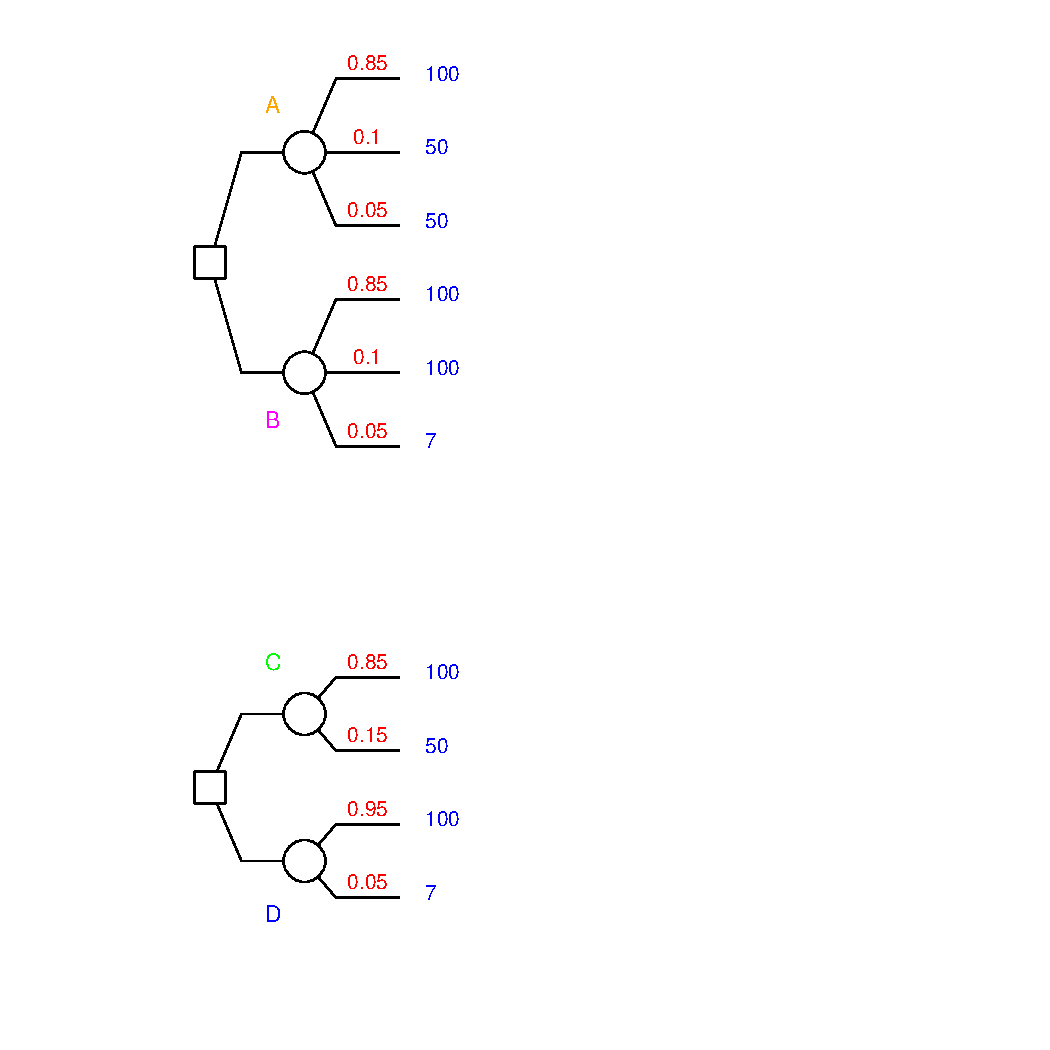
\includegraphics[width=0.8\linewidth]{figure/unnamed-chunk-43} 

}



\end{knitrout}


With $81$ participants, $51.9\%$ preferred $A > B$, $85.2\%$ preferred $D > C$ and $63\%$ preferred $F > E$. The PT predictions can be generated via the following code.

\begin{knitrout}
\definecolor{shadecolor}{rgb}{0.969, 0.969, 0.969}\color{fgcolor}\begin{kframe}
\begin{alltt}
\hlstd{tk_1992_utility} \hlkwb{<-} \hlkwd{Utility}\hlstd{(}\hlkwc{fun}\hlstd{=}\hlstr{"power"}\hlstd{,} \hlkwc{par}\hlstd{=}\hlkwd{c}\hlstd{(}\hlkwc{alpha}\hlstd{=}\hlnum{0.88}\hlstd{,} \hlkwc{beta}\hlstd{=}\hlnum{0.88}\hlstd{,} \hlkwc{lambda}\hlstd{=}\hlnum{2.25}\hlstd{))}
\hlstd{tk_1992_positive_prob_weight} \hlkwb{<-} \hlkwd{ProbWeight}\hlstd{(}\hlkwc{fun}\hlstd{=}\hlstr{"Tversky_Kahneman_1992"}\hlstd{,} \hlkwc{par}\hlstd{=}\hlkwd{c}\hlstd{(}\hlkwc{alpha}\hlstd{=}\hlnum{0.61}\hlstd{))}
\hlstd{tk_1992_negative_prob_weight} \hlkwb{<-} \hlkwd{ProbWeight}\hlstd{(}\hlkwc{fun}\hlstd{=}\hlstr{"Tversky_Kahneman_1992"}\hlstd{,} \hlkwc{par}\hlstd{=}\hlkwd{c}\hlstd{(}\hlkwc{alpha}\hlstd{=}\hlnum{0.69}\hlstd{))}
\hlkwd{comparePT}\hlstd{(my_choices,}
        \hlkwc{prob_weight_for_positive_outcomes}\hlstd{=tk_1992_positive_prob_weight,}
        \hlkwc{prob_weight_for_negative_outcomes}\hlstd{=tk_1992_negative_prob_weight,}
        \hlkwc{utility}\hlstd{=tk_1992_utility,} \hlkwc{digits}\hlstd{=}\hlnum{4}\hlstd{)}
\end{alltt}
\begin{verbatim}
##   cid gid    ev     pt     ce     rp
## 1   1   1   600 -523.3 -488.9   1089
## 2   1   2   750 -742.8   -728   1478
## 3   2   1  2100  649.2   1570  530.1
## 4   2   2  2250  652.3   1578  671.6
## 5   3   1 -1500  -1172  -1223 -277.1
## 6   3   2 -1500  -1395  -1490 -9.982
\end{verbatim}
\end{kframe}
\end{knitrout}


With the parameterisations from \cite{Tversky_Kahneman_1992}, PT correctly predicts the preferences $A > B$ and $D > C$, but incorrectly predicts $E > F$.
The predictions for TAX are generated via the following code.

\begin{knitrout}
\definecolor{shadecolor}{rgb}{0.969, 0.969, 0.969}\color{fgcolor}\begin{kframe}
\begin{alltt}
\hlstd{my_utility} \hlkwb{<-} \hlkwd{Utility}\hlstd{(}\hlkwc{fun}\hlstd{=}\hlstr{"linear"}\hlstd{,} \hlkwc{par}\hlstd{=}\hlkwd{c}\hlstd{(}\hlkwc{lambda}\hlstd{=}\hlnum{1}\hlstd{))}
\hlstd{power_prob_weight} \hlkwb{<-} \hlkwd{ProbWeight}\hlstd{(}\hlkwc{fun}\hlstd{=}\hlstr{"power"}\hlstd{,} \hlkwc{par}\hlstd{=}\hlkwd{c}\hlstd{(}\hlkwc{alpha}\hlstd{=}\hlnum{0.7}\hlstd{,} \hlkwc{beta}\hlstd{=}\hlnum{1}\hlstd{))}
\hlkwd{compareTAX}\hlstd{(my_choices,} \hlkwc{prob_weight}\hlstd{=power_prob_weight,} \hlkwc{utility}\hlstd{=my_utility,} \hlkwc{delta}\hlstd{=}\hlopt{-}\hlnum{1}\hlstd{,} \hlkwc{digits}\hlstd{=}\hlnum{4}\hlstd{)}
\end{alltt}
\begin{verbatim}
##   cid gid    ev   tax    ce     rp
## 1   1   1   600  -600  -600   1200
## 2   1   2   750 -1900 -1900   2650
## 3   2   1  2100  1400  1400    700
## 4   2   2  2250  1367  1367  883.4
## 5   3   1 -1500 -1000 -1000   -500
## 6   3   2 -1500 -1267 -1267 -233.2
\end{verbatim}
\end{kframe}
\end{knitrout}


TAX correctly predicts $A > B$ and $E > F$, but incorrectly predicts $C > D$.

\subsection{Violations of coalescing}

PT assumes gamble outcomes with the same objective consequences can be coalesced without affecting choice preferences. \cite{Birnbaum_2004}, however, identified situations
where this was not true for the majority of decision makers. Consider problems 14 and 8 from \citet[][Table 3 p. 95]{Birnbaum_2004} which are tests of coalescing.

\begin{knitrout}
\definecolor{shadecolor}{rgb}{0.969, 0.969, 0.969}\color{fgcolor}\begin{kframe}
\begin{alltt}
\hlstd{choice_ids} \hlkwb{<-} \hlkwd{c}\hlstd{(}\hlnum{1}\hlstd{,} \hlnum{1}\hlstd{,} \hlnum{1}\hlstd{,} \hlnum{1}\hlstd{,} \hlnum{1}\hlstd{,} \hlnum{1}\hlstd{,} \hlnum{2}\hlstd{,} \hlnum{2}\hlstd{,} \hlnum{2}\hlstd{,} \hlnum{2}\hlstd{)}
\hlstd{gamble_ids} \hlkwb{<-} \hlkwd{c}\hlstd{(}\hlnum{1}\hlstd{,} \hlnum{1}\hlstd{,} \hlnum{1}\hlstd{,} \hlnum{2}\hlstd{,} \hlnum{2}\hlstd{,} \hlnum{2}\hlstd{,} \hlnum{1}\hlstd{,} \hlnum{1}\hlstd{,} \hlnum{2}\hlstd{,} \hlnum{2}\hlstd{)}
\hlstd{outcome_ids} \hlkwb{<-} \hlkwd{c}\hlstd{(}\hlnum{1}\hlstd{,} \hlnum{2}\hlstd{,} \hlnum{3}\hlstd{,} \hlnum{1}\hlstd{,} \hlnum{2}\hlstd{,} \hlnum{3}\hlstd{,} \hlnum{1}\hlstd{,} \hlnum{2}\hlstd{,} \hlnum{1}\hlstd{,} \hlnum{2}\hlstd{)}
\hlstd{objective_consequences} \hlkwb{<-} \hlkwd{c}\hlstd{(}\hlnum{100}\hlstd{,} \hlnum{50}\hlstd{,} \hlnum{50}\hlstd{,}
        \hlnum{100}\hlstd{,} \hlnum{100}\hlstd{,} \hlnum{7}\hlstd{,}
        \hlnum{100}\hlstd{,} \hlnum{50}\hlstd{,} \hlnum{100}\hlstd{,} \hlnum{7}\hlstd{)}
\hlstd{probability_strings} \hlkwb{<-} \hlkwd{c}\hlstd{(}\hlstr{"0.85"}\hlstd{,} \hlstr{"0.1"}\hlstd{,} \hlstr{"0.05"}\hlstd{,}
        \hlstr{"0.85"}\hlstd{,} \hlstr{"0.1"}\hlstd{,} \hlstr{"0.05"}\hlstd{,}
        \hlstr{"0.85"}\hlstd{,} \hlstr{"0.15"}\hlstd{,} \hlstr{"0.95"}\hlstd{,} \hlstr{"0.05"}\hlstd{)}
\hlstd{my_choices} \hlkwb{<-} \hlkwd{Choices}\hlstd{(}\hlkwc{choice_ids}\hlstd{=choice_ids,}
        \hlkwc{gamble_ids}\hlstd{=gamble_ids,}
        \hlkwc{outcome_ids}\hlstd{=outcome_ids,}
        \hlkwc{objective_consequences}\hlstd{=objective_consequences,}
        \hlkwc{probability_strings}\hlstd{=probability_strings)}
\hlstd{my_choices}
\end{alltt}
\begin{verbatim}
##    cid gid oid   pr  oc
## 1    1   1   1 0.85 100
## 2    1   1   2  0.1  50
## 3    1   1   3 0.05  50
## 4    1   2   1 0.85 100
## 5    1   2   2  0.1 100
## 6    1   2   3 0.05   7
## 7    2   1   1 0.85 100
## 8    2   1   2 0.15  50
## 9    2   2   1 0.95 100
## 10   2   2   2 0.05   7
\end{verbatim}
\begin{alltt}
\hlkwd{drawChoices}\hlstd{(my_choices,}
        \hlkwc{decision_square_x}\hlstd{=}\hlnum{0.2}\hlstd{,} \hlkwc{decision_square_edge_length}\hlstd{=}\hlnum{0.03}\hlstd{,}
        \hlkwc{circle_radius}\hlstd{=}\hlnum{0.02}\hlstd{,} \hlkwc{y_split_gap}\hlstd{=}\hlnum{0.07}\hlstd{,} \hlkwc{x_split_offset}\hlstd{=}\hlnum{0.03}\hlstd{,}
        \hlkwc{probability_text_digits}\hlstd{=}\hlnum{4}\hlstd{,} \hlkwc{y_probability_text_offset}\hlstd{=}\hlnum{0.015}\hlstd{,}
        \hlkwc{y_value_text_offset}\hlstd{=}\hlnum{0.005}\hlstd{,} \hlkwc{x_value_text_offset}\hlstd{=}\hlnum{0.025}\hlstd{,}
        \hlkwc{probability_text_font_colour}\hlstd{=}\hlstr{"red"}\hlstd{,} \hlkwc{probability_text_font_size}\hlstd{=}\hlnum{10}\hlstd{,}
        \hlkwc{objective_consequence_text_font_colour}\hlstd{=}\hlstr{"blue"}\hlstd{,}
        \hlkwc{objective_consequence_text_font_size}\hlstd{=}\hlnum{10}\hlstd{,}
        \hlkwc{label}\hlstd{=}\hlkwd{c}\hlstd{(}\hlstr{"A"}\hlstd{,}\hlstr{"B"}\hlstd{,}\hlstr{"C"}\hlstd{,}\hlstr{"D"}\hlstd{),}
        \hlkwc{label_font_colour}\hlstd{=}\hlkwd{c}\hlstd{(}\hlstr{"orange"}\hlstd{,}\hlstr{"magenta"}\hlstd{,}\hlstr{"green"}\hlstd{,}\hlstr{"blue"}\hlstd{),}
        \hlkwc{label_font_size}\hlstd{=}\hlkwd{c}\hlstd{(}\hlnum{11}\hlstd{,}\hlnum{11}\hlstd{,}\hlnum{11}\hlstd{,}\hlnum{11}\hlstd{),}
        \hlkwc{label_positions}\hlstd{=}\hlkwd{list}\hlstd{(}\hlkwd{c}\hlstd{(}\hlnum{0.26}\hlstd{,}\hlnum{0.9}\hlstd{),}\hlkwd{c}\hlstd{(}\hlnum{0.26}\hlstd{,}\hlnum{0.6}\hlstd{),}
                \hlkwd{c}\hlstd{(}\hlnum{0.26}\hlstd{,}\hlnum{0.37}\hlstd{),}\hlkwd{c}\hlstd{(}\hlnum{0.26}\hlstd{,}\hlnum{0.13}\hlstd{)))}
\end{alltt}
\end{kframe}

{\centering 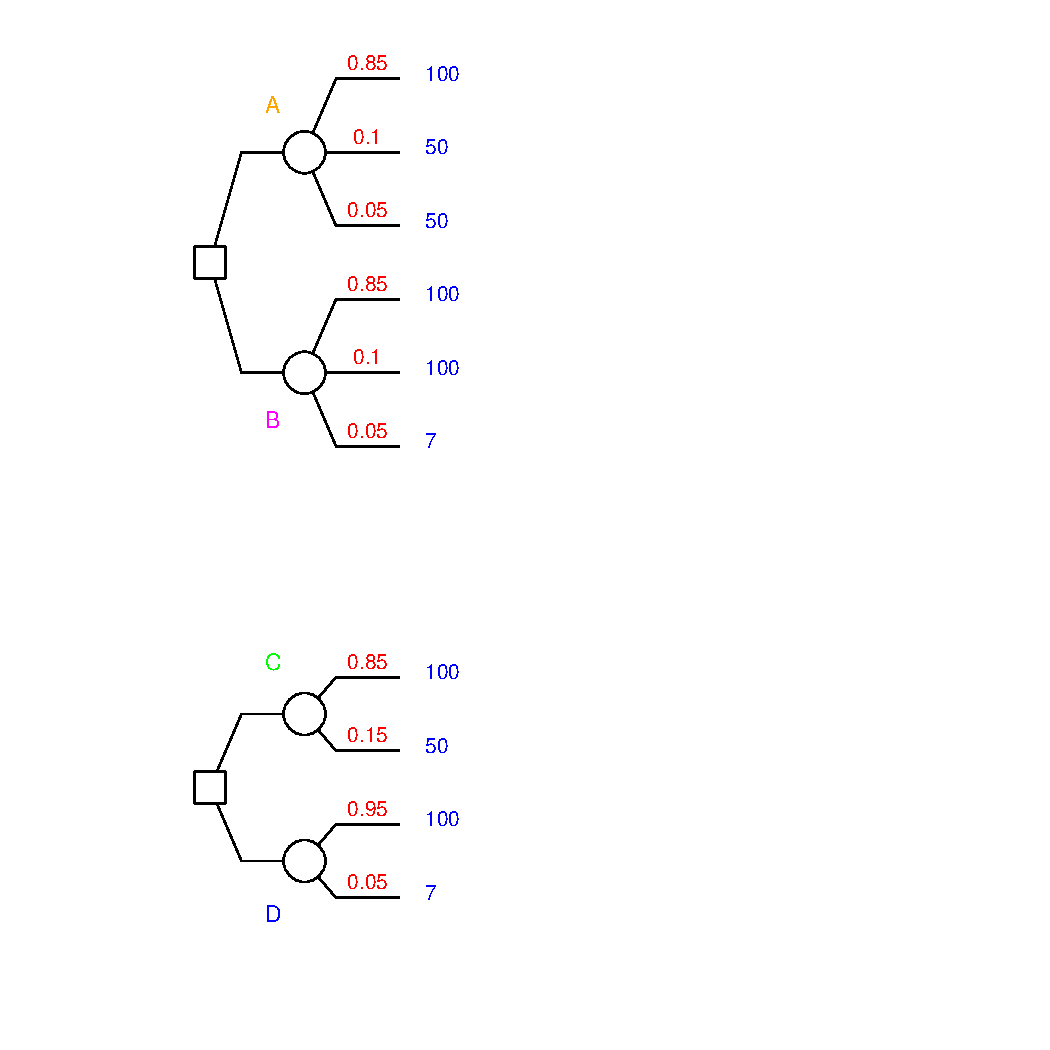
\includegraphics[width=0.8\linewidth]{figure/unnamed-chunk-46} 

}



\end{knitrout}


In a sample of $100$ participants, $63\%$ preferred $B > A$ and $75\%$ preferred $C > D$ \cite[][Table 3 p. 95 (unframed condition)]{Birnbaum_2004}. However, PT incorrectly predicts the preferences $A > B$ and $C > D$.

\begin{knitrout}
\definecolor{shadecolor}{rgb}{0.969, 0.969, 0.969}\color{fgcolor}\begin{kframe}
\begin{alltt}
\hlstd{tk_1992_utility} \hlkwb{<-} \hlkwd{Utility}\hlstd{(}\hlkwc{fun}\hlstd{=}\hlstr{"power"}\hlstd{,} \hlkwc{par}\hlstd{=}\hlkwd{c}\hlstd{(}\hlkwc{alpha}\hlstd{=}\hlnum{0.88}\hlstd{,} \hlkwc{beta}\hlstd{=}\hlnum{0.88}\hlstd{,} \hlkwc{lambda}\hlstd{=}\hlnum{2.25}\hlstd{))}
\hlstd{tk_1992_positive_prob_weight} \hlkwb{<-} \hlkwd{ProbWeight}\hlstd{(}\hlkwc{fun}\hlstd{=}\hlstr{"Tversky_Kahneman_1992"}\hlstd{,} \hlkwc{par}\hlstd{=}\hlkwd{c}\hlstd{(}\hlkwc{alpha}\hlstd{=}\hlnum{0.61}\hlstd{))}
\hlstd{tk_1992_negative_prob_weight} \hlkwb{<-} \hlkwd{ProbWeight}\hlstd{(}\hlkwc{fun}\hlstd{=}\hlstr{"Tversky_Kahneman_1992"}\hlstd{,} \hlkwc{par}\hlstd{=}\hlkwd{c}\hlstd{(}\hlkwc{alpha}\hlstd{=}\hlnum{0.69}\hlstd{))}
\hlkwd{comparePT}\hlstd{(my_choices,}
        \hlkwc{prob_weight_for_positive_outcomes}\hlstd{=tk_1992_positive_prob_weight,}
        \hlkwc{prob_weight_for_negative_outcomes}\hlstd{=tk_1992_negative_prob_weight,}
        \hlkwc{utility}\hlstd{=tk_1992_utility,} \hlkwc{digits}\hlstd{=}\hlnum{4}\hlstd{)}
\end{alltt}
\begin{verbatim}
##   cid gid    ev    pt    ce    rp
## 1   1   1  92.5 48.44 82.23 10.27
## 2   1   2 95.35 46.79 79.05  16.3
## 3   2   1  92.5 48.44 82.23 10.27
## 4   2   2 95.35 46.79 79.05  16.3
\end{verbatim}
\end{kframe}
\end{knitrout}


For these choices TAX correctly predicts the preferences $B > A$ and $C > D$.

\begin{knitrout}
\definecolor{shadecolor}{rgb}{0.969, 0.969, 0.969}\color{fgcolor}\begin{kframe}
\begin{alltt}
\hlstd{my_utility} \hlkwb{<-} \hlkwd{Utility}\hlstd{(}\hlkwc{fun}\hlstd{=}\hlstr{"linear"}\hlstd{,} \hlkwc{par}\hlstd{=}\hlkwd{c}\hlstd{(}\hlkwc{lambda}\hlstd{=}\hlnum{2.25}\hlstd{))}
\hlstd{power_prob_weight} \hlkwb{<-} \hlkwd{ProbWeight}\hlstd{(}\hlkwc{fun}\hlstd{=}\hlstr{"power"}\hlstd{,} \hlkwc{par}\hlstd{=}\hlkwd{c}\hlstd{(}\hlkwc{alpha}\hlstd{=}\hlnum{0.7}\hlstd{,} \hlkwc{beta}\hlstd{=}\hlnum{1}\hlstd{))}
\hlkwd{compareTAX}\hlstd{(my_choices,} \hlkwc{prob_weight}\hlstd{=power_prob_weight,} \hlkwc{utility}\hlstd{=my_utility,} \hlkwc{delta}\hlstd{=}\hlopt{-}\hlnum{1}\hlstd{,} \hlkwc{digits}\hlstd{=}\hlnum{4}\hlstd{)}
\end{alltt}
\begin{verbatim}
##   cid gid    ev   tax    ce    rp
## 1   1   1  92.5 68.37 68.37 24.13
## 2   1   2 95.35  69.7  69.7 25.65
## 3   2   1  92.5  75.7  75.7  16.8
## 4   2   2 95.35    62    62 33.35
\end{verbatim}
\end{kframe}
\end{knitrout}



\subsection{Violations of first-order stochastic dominance}

\citet[p. 263-264]{Birnbaum_2005b} defines first-order stochastic dominance for two different gambles $A$ and $B$
with $A$ stochastically dominating $B$ as ``the probability of winning prize x or greater given gamble A is greater than or
equal to the probability to win x or more in gamble B, for all x, and if this probability is
strictly higher for at least one value of x".
\citet[][p. 221]{Yates_1990} provides an intuitive definition of dominance as follows: ``One alternative is said to dominate another if it is just as good on all
the pertinent aspect dimensions and better on at least one".
Prospect theory assumes decision makers satisfy first-order stochastic dominance at all times, if it is
detected.
\citet[][p. 74]{Birnbaum_1997} created a recipe for gambles where first order stochastic dominance is systematically
violated in choices between the gambles. These were empirically investigated in \citet[][]{Birnbaum_Navarrete_1998}. 
{\bf pt} can be used to create choices using this recipe.

\begin{knitrout}
\definecolor{shadecolor}{rgb}{0.969, 0.969, 0.969}\color{fgcolor}\begin{kframe}
\begin{alltt}
\hlstd{my_list} \hlkwb{<-} \hlkwd{vsdChoices}\hlstd{(}\hlkwc{x}\hlstd{=}\hlnum{12}\hlstd{,} \hlkwc{y}\hlstd{=}\hlnum{96}\hlstd{,} \hlkwc{p}\hlstd{=}\hlstr{"0.1"}\hlstd{,} \hlkwc{q}\hlstd{=}\hlstr{"0.9"}\hlstd{,} \hlkwc{x_plus}\hlstd{=}\hlnum{14}\hlstd{,} \hlkwc{y_minus}\hlstd{=}\hlnum{90}\hlstd{,} \hlkwc{r}\hlstd{=}\hlstr{"0.05"}\hlstd{)}
\hlstd{my_list}
\end{alltt}
\begin{verbatim}
## $g0
##   cid gid oid  pr oc
## 1   1   1   1 0.1 12
## 2   1   1   2 0.9 96
## 
## $gplusminus
##   cid gid oid   pr oc
## 1   1   1   1 0.05 12
## 2   1   1   2 0.05 14
## 3   1   1   3  0.9 96
## 4   1   2   1  0.1 12
## 5   1   2   2 0.05 90
## 6   1   2   3 0.85 96
## 
## $gsplusminus
##   cid gid oid   pr oc
## 1   1   1   1 0.05 12
## 2   1   1   2 0.05 14
## 3   1   1   3 0.05 96
## 4   1   1   4 0.85 96
## 5   1   2   1 0.05 12
## 6   1   2   2 0.05 12
## 7   1   2   3 0.05 90
## 8   1   2   4 0.85 96
\end{verbatim}
\begin{alltt}
\hlkwd{drawChoices}\hlstd{(my_list[[}\hlnum{2}\hlstd{]],}
        \hlkwc{decision_square_x}\hlstd{=}\hlnum{0.2}\hlstd{,} \hlkwc{decision_square_edge_length}\hlstd{=}\hlnum{0.05}\hlstd{,}
        \hlkwc{circle_radius}\hlstd{=}\hlnum{0.025}\hlstd{,} \hlkwc{y_split_gap}\hlstd{=}\hlnum{0.1}\hlstd{,} \hlkwc{x_split_offset}\hlstd{=}\hlnum{0.03}\hlstd{,}
        \hlkwc{probability_text_digits}\hlstd{=}\hlnum{4}\hlstd{,} \hlkwc{y_probability_text_offset}\hlstd{=}\hlnum{0.015}\hlstd{,}
        \hlkwc{y_value_text_offset}\hlstd{=}\hlnum{0.005}\hlstd{,} \hlkwc{x_value_text_offset}\hlstd{=}\hlnum{0.025}\hlstd{,}
        \hlkwc{probability_text_font_colour}\hlstd{=}\hlstr{"red"}\hlstd{,} \hlkwc{probability_text_font_size}\hlstd{=}\hlnum{11}\hlstd{,}
        \hlkwc{objective_consequence_text_font_colour}\hlstd{=}\hlstr{"blue"}\hlstd{,}
        \hlkwc{objective_consequence_text_font_size}\hlstd{=}\hlnum{11}\hlstd{,} \hlkwc{label}\hlstd{=}\hlkwd{c}\hlstd{(}\hlstr{"A"}\hlstd{,}\hlstr{"B"}\hlstd{),}
        \hlkwc{label_font_colour}\hlstd{=}\hlkwd{c}\hlstd{(}\hlstr{"orange"}\hlstd{,}\hlstr{"magenta"}\hlstd{),} \hlkwc{label_font_size}\hlstd{=}\hlkwd{c}\hlstd{(}\hlnum{11}\hlstd{,}\hlnum{11}\hlstd{),}
        \hlkwc{label_positions}\hlstd{=}\hlkwd{list}\hlstd{(}\hlkwd{c}\hlstd{(}\hlnum{0.26}\hlstd{,}\hlnum{0.7}\hlstd{),}\hlkwd{c}\hlstd{(}\hlnum{0.26}\hlstd{,}\hlnum{0.3}\hlstd{)))}
\end{alltt}
\end{kframe}

{\centering 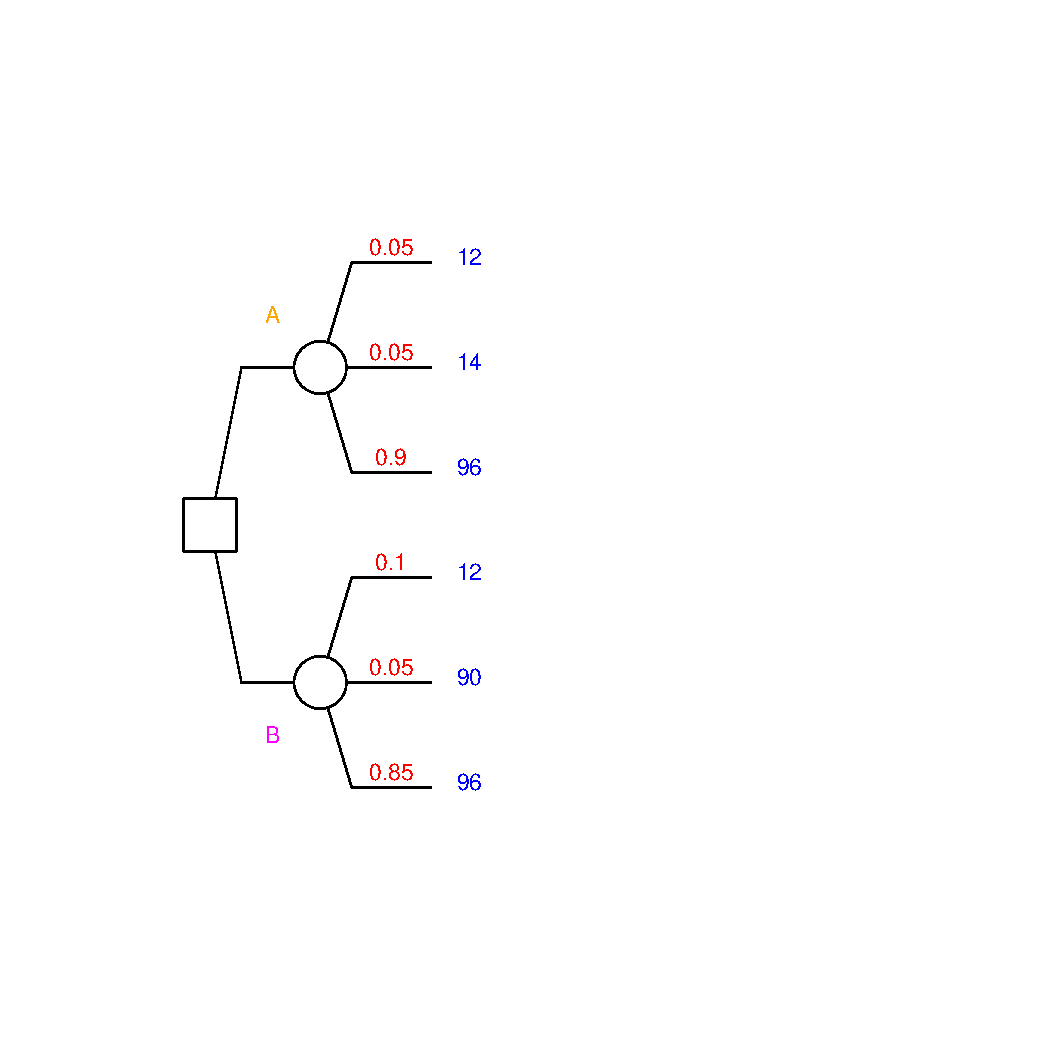
\includegraphics[width=0.8\linewidth]{figure/unnamed-chunk-49} 

}



\end{knitrout}


In this case gamble $A$ stochastically dominates gamble $B$. This can be seen by calculating the probability of receiving an amount greater than or equal to each objective consequence of $A$ and $B$, depicted in
Table \ref{stochastic_dominance_table}. For the amounts $96$ and $14$, $A$ dominates $B$. For the amounts $90$ and
$12$, $A$ has probabilities at least the same as $B$.

\begin{table}[!h]
\caption{Gamble $A$ stochastically dominates gamble $B$.}
\centering
\begin{tabular}{ l l c l l }
\hline
A &   &   & B &   \\
\hline
oc & pr  &   & oc & pr  \\
\hline
96 & 0.9 & $>$ & 96 & 0.85 \\
90 & 0.9 & same & 90 & 0.9 \\
14 & 0.95 & $>$ & 14 & 0.9 \\
12 & 1.0 & same & 12 & 1.0 \\
\hline
\end{tabular}
\label{stochastic_dominance_table}
\end{table}

However, \citet[][Table 1 p. 61]{Birnbaum_Navarrete_1998} found in $100$ participants, $73\%$ preferred $B > A$.
For any set of functional forms and parameterisations, PT predicts $A > B$.

\begin{knitrout}
\definecolor{shadecolor}{rgb}{0.969, 0.969, 0.969}\color{fgcolor}\begin{kframe}
\begin{alltt}
\hlstd{tk_1992_utility} \hlkwb{<-} \hlkwd{Utility}\hlstd{(}\hlkwc{fun}\hlstd{=}\hlstr{"power"}\hlstd{,} \hlkwc{par}\hlstd{=}\hlkwd{c}\hlstd{(}\hlkwc{alpha}\hlstd{=}\hlnum{0.88}\hlstd{,} \hlkwc{beta}\hlstd{=}\hlnum{0.88}\hlstd{,} \hlkwc{lambda}\hlstd{=}\hlnum{2.25}\hlstd{))}
\hlstd{linear_in_log_odds_prob_weight} \hlkwb{<-} \hlkwd{ProbWeight}\hlstd{(}\hlkwc{fun}\hlstd{=}\hlstr{"linear_in_log_odds"}\hlstd{,} \hlkwc{par}\hlstd{=}\hlkwd{c}\hlstd{(}\hlkwc{alpha}\hlstd{=}\hlnum{0.61}\hlstd{,} \hlkwc{beta}\hlstd{=}\hlnum{0.724}\hlstd{))}
\hlkwd{comparePT}\hlstd{(my_list[[}\hlnum{2}\hlstd{]],}
        \hlkwc{prob_weight_for_positive_outcomes}\hlstd{=linear_in_log_odds_prob_weight,}
        \hlkwc{prob_weight_for_negative_outcomes}\hlstd{=linear_in_log_odds_prob_weight,}
        \hlkwc{utility}\hlstd{=tk_1992_utility,} \hlkwc{digits}\hlstd{=}\hlnum{4}\hlstd{)}
\end{alltt}
\begin{verbatim}
##   cid gid   ev    pt    ce    rp
## 1   1   1 87.7 43.24 72.27 15.43
## 2   1   2 87.3 42.96 71.73 15.57
\end{verbatim}
\end{kframe}
\end{knitrout}


However TAX predicts $B > A$.

\begin{knitrout}
\definecolor{shadecolor}{rgb}{0.969, 0.969, 0.969}\color{fgcolor}\begin{kframe}
\begin{alltt}
\hlstd{my_utility} \hlkwb{<-} \hlkwd{Utility}\hlstd{(}\hlkwc{fun}\hlstd{=}\hlstr{"linear"}\hlstd{,} \hlkwc{par}\hlstd{=}\hlkwd{c}\hlstd{(}\hlkwc{lambda}\hlstd{=}\hlnum{1.0}\hlstd{))}
\hlstd{power_prob_weight} \hlkwb{<-} \hlkwd{ProbWeight}\hlstd{(}\hlkwc{fun}\hlstd{=}\hlstr{"power"}\hlstd{,} \hlkwc{par}\hlstd{=}\hlkwd{c}\hlstd{(}\hlkwc{alpha}\hlstd{=}\hlnum{0.7}\hlstd{,} \hlkwc{beta}\hlstd{=}\hlnum{1}\hlstd{))}
\hlkwd{compareTAX}\hlstd{(my_list[[}\hlnum{2}\hlstd{]],} \hlkwc{prob_weight}\hlstd{=power_prob_weight,} \hlkwc{utility}\hlstd{=my_utility,} \hlkwc{delta}\hlstd{=}\hlopt{-}\hlnum{1}\hlstd{,} \hlkwc{digits}\hlstd{=}\hlnum{4}\hlstd{)}
\end{alltt}
\begin{verbatim}
##   cid gid   ev   tax    ce    rp
## 1   1   1 87.7 45.77 45.77 41.93
## 2   1   2 87.3  63.1  63.1  24.2
\end{verbatim}
\end{kframe}
\end{knitrout}


Whereas under PT stochastic dominance is always obeyed, other theories such as TAX can predict violations of stochastic dominance under certain conditions with stochastic dominance being obeyed most of the time. \cite{Levy_2008} explains these violations as effects of bounded rationality. In his experiments
the more transparent he made the first-order stochastic dominance, the fewer violations he detected.

\section{Summary}

As new risky decision making theories are developed, they can be incorporated into the R package {\bf pt} for comparison with the currently implemented theories. This will allow a computational library to be developed to support decision making research. The package can be used to facilitate Gedanken experiments for developing new critical tests of decision making. The intention is to provide computational insights to develop theories of risky decision making that can more accurately account for empirical data than current theories, and to generate ideas for novel predictions.

\section*{Acknowledgments}

The author would like to thank Peter Wakker for comments on an earlier manuscript and calling attention to the basic
prospect theory calculator available on his homepage at 
\url{http://people.few.eur.nl/wakker/miscella/calculate.cpt.kobb/index.htm}, and Vitalie Spinu for helpful discussions around the package design and suggesting improvements to the R code.


\bibliographystyle{apalike}
\bibliography{pt_vignette}

\end{document}
